\documentclass[conf]{new-aiaa}
%\documentclass[journal]{new-aiaa} for journal papers
\usepackage[utf8]{inputenc}

\usepackage{graphicx}
\usepackage{amsmath}
\usepackage[version=4]{mhchem}
\usepackage{siunitx}
\usepackage{longtable,tabularx}
\setlength\LTleft{0pt} 

\usepackage{amssymb,url,times,gensymb}%,subfigure}% amsthm is the one!
\usepackage{caption,subcaption,hyperref}
\usepackage{color,comment}

\newtheorem{prop}{Proposition}
\newcommand{\norm}[1]{\ensuremath{\left\| #1 \right\|}}
\newcommand{\abs}[1]{\ensuremath{\left| #1 \right|}}
\newcommand{\bracket}[1]{\ensuremath{\left[ #1 \right]}}
\newcommand{\braces}[1]{\ensuremath{\left\{ #1 \right\}}}
\newcommand{\parenth}[1]{\ensuremath{\left( #1 \right)}}
\newcommand{\ip}[1]{\ensuremath{\langle #1 \rangle}}
\newcommand{\refeqn}[1]{(\ref{eqn:#1})}
\newcommand{\reffig}[1]{Figure \ref{fig:#1}}
\newcommand{\tr}[1]{\mbox{tr}\ensuremath{\negthickspace\bracket{#1}}}
\newcommand{\trs}[1]{\mbox{tr}\ensuremath{\!\bracket{#1}}}
\newcommand{\deriv}[2]{\ensuremath{\frac{\partial #1}{\partial #2}}}
\newcommand{\G}{\ensuremath{\mathsf{G}}}
\newcommand{\SO}{\ensuremath{\mathsf{SO(3)}}}
\newcommand{\T}{\ensuremath{\mathsf{T}}}
\renewcommand{\L}{\ensuremath{\mathsf{L}}}
\newcommand{\so}{\ensuremath{\mathfrak{so}(3)}}
\newcommand{\SE}{\ensuremath{\mathsf{SE(3)}}}
\newcommand{\se}{\ensuremath{\mathfrak{se}(3)}}
\renewcommand{\Re}{\ensuremath{\mathbb{R}}}
\newcommand{\Sph}{\ensuremath{\mathsf{S}}}
\newcommand{\aSE}[2]{\ensuremath{\begin{bmatrix}#1&#2\\0&1\end{bmatrix}}}
\newcommand{\ase}[2]{\ensuremath{\begin{bmatrix}#1&#2\\0&0\end{bmatrix}}}
\newcommand{\D}{\ensuremath{\mathbf{D}}}
\renewcommand{\d}{\ensuremath{\mathbf{d}}}
\newcommand{\pair}[1]{\ensuremath{\left\langle #1 \right\rangle}}
\newcommand{\met}[1]{\ensuremath{\langle\!\langle #1 \rangle\!\rangle}}
\newcommand{\Ad}{\ensuremath{\mathrm{Ad}}}
\newcommand{\ad}{\ensuremath{\mathrm{ad}}}
\newcommand{\g}{\ensuremath{\mathfrak{g}}}
\newcommand{\argmin}{\operatornamewithlimits{argmin}}
\newcommand{\argmax}{\operatornamewithlimits{argmax}}
\graphicspath{{../../Fig/}}

\newcommand{\todo}[1]{\vspace{5 mm}\par \noindent
\marginpar{\textsc{ToDo}} \framebox{\begin{minipage}[c]{0.95
\textwidth} \tt #1 \end{minipage}}\vspace{5 mm}\par}
%\newcommand{\todo}[1]{}

\title{Autonomous Aerial Exploration for Topological Mapping of Mars Environments}

<<<<<<< HEAD
\author{Evan Kaufman\footnote{Graduate Research Assistant, Department of Mechanical and Aerospace Engineering, The George Washington University, 800 22nd St NW, Washington, DC, 20052} and Taeyoung Lee\footnote{Associate Professor, Department of Mechanical and Aerospace Engineering, The George Washington University, 800 22nd St NW, Washington, DC, 20052}}% TODO: update if AIAA member
\affil{The George Washington University, Washington, DC, 20052}
% TODO: funding source
=======
\author{Evan Kaufman\footnote{Graduate Research Assistant, Department of Mechanical and Aerospace Engineering, The George Washington University, 800 22nd St NW, Washington, DC, 20052} and Taeyoung Lee\footnote{Associate Professor, Department of Mechanical and Aerospace Engineering, The George Washington University, 800 22nd St NW, Washington, DC, 20052}}
\affil{The George Washington University, Washington, DC, 20052}
>>>>>>> evan

\begin{document}

\maketitle

\begin{abstract}
This paper proposes a 3D autonomous exploration scheme designed for a flying vehicle to build a topological map representing the complex environment of the surface of Mars. 
The environment is modeled as a uniform grid, and the measurements from depth scans are utilized to determine the probability of occupancy at every cell within the scanned area. 
Shannon's entropy serves as a measure of map uncertainty, where the motion of the aerial vehicle is guided to minimize entropy, thereby maximizing map information. We propose a novel technique to predict future map entropy from depth sensors capable of scanning 3D spaces, and formulate autonomous exploration as an optimization problem based on map information gain subject to inequality constraints to avoid collision. The proposed approach is demonstrated with numerical simulations using contour data from the surface of Mars.
\end{abstract}


\section{Introduction}

The topography of Mars has several benefits in future mission planning for landing spacecraft and  image distortion correction, among other research objectives. The Mars Orbiting Laser Altimeter (MOLA) mission greatly improved the topography map of the surface, but was limited to an uncertainty of roughly eight meters~\cite{MOLA99}. The only precise topography knowledge about the surface comes from four rovers, two of which are inactive, and have covered only a small portion of the surface area of Mars.

Mapping and exploring Mars presents several challenges. Existing rovers are ground vehicles, incapable of traversing steep or dangerous terrain. Flying vehicles avoid this restriction, but special attention must be placed on their motion planning in this uncertain environment. Humans cannot directly give commands to the vehicles due to the signal time delay between Mars and Earth. Even if a humans are present on Mars, they can only provide sub-optimal motion commands on a small scale. These challenges motivate an autonomous approach to 3D mapping and exploration in uncertain and complex environments for a flying vehicle near the surface of Mars.

The study of 3D mapping and autonomous exploration has received substantial attention for applications on Earth. Occupancy grid mapping in 3D is a popular approach where an environment is decomposed into evenly-spaced cubic grid cells, where each cell is assumed as occupied or free~\cite{ThrBurFox05,WurHorBenStaBur10}. The goal is finding the probability of each cell being occupied. An exact solution of this probability was recently found by the authors using the stochastic properties of onboard sensors directly~\cite{KauLeeAiMos16,KauTakAiLee17}. Using an exact occupancy grid mapping algorithm in 3D, the topological information of the surface of Mars can be accurately computed in real-time.

Next, the robot must determine motions based on how much mapping knowledge it expects to gain, known as autonomous exploration. The most popular approach to this problem is known as frontier-based exploration~\cite{ZhuDinLinWu15,SenWan16,KleDor13}. The main idea is that the robot moves through previously-mapped free space toward the boundary between free space and uncertain space, known as a frontier. The robot takes measurements of this frontier, thereby pushing back the boundary. This process is repeated until the map is well-known. Despite the intuitive nature of this approach, there is no measure or prediction of how these robotic actions improve map information. Thus, frontier-based approaches rely on a heuristic rule, and are inherently suboptimal.

In contrast, entropy-based autonomous exploration approaches seek to minimize future map uncertainty. Shannon's entropy is a measure of map uncertainty; since minimizing future map uncertainty is equivalent to maximizing map information gain, these approaches select robotic actions to minimize entropy~\cite{StaGriBur05}. In~\cite{KauAiLee16}, an exact solution to expected entropy was developed, and in~\cite{KauTakAiLee18}, this concept is extended to 3D office-like environments assuming the environment can be approximated as vertically-uniform. Similarly, \cite{MauDakPet14} simplifies tasks by decomposing the 3D space into rooms. While these approaches can be effective for buildings, they are incompatible with the surface of Mars, which has complicated geological features that require careful consideration.

In this paper, we propose a 3D autonomous exploration algorithm that considers the 3D probabilistic occupancy grid map and sensor properties explicitly. The complicated and uncertain geometry of the surface of Mars is captured by aerial mapping because this approach can cover a large area effectively. An onboard depth sensor, such as a 3D laser scanner, gathers range measurements to determine the occupancy probabilities of 3D grid cells. Then, collision-free future pose candidates are considered. The predicted negative entropy changes from measurements passing through 3D space are maximized while also considering travel costs. The aerial vehicle then uses Dijkstra's search in 3D for collision-free motion planning, and the complete process follows a receding-horizon framework for consistently using updated information. The proposed optimal approach is designed specifically for real-time exploration of the surface of Mars, where the flying robot mostly maps occupied space below the vehicle, but is also capable of looking ahead to capture steep and quickly-changing terrain. In short, the proposed autonomous exploration approach predicts future map uncertainty in 3D space to determine optimal actions that maximize map information gain while avoiding collisions.

The paper is organized as follows. The mapping probability and expected entropy calculation are defined in Section \ref{sec:ProbDef}. The proposed 3D exploration for information gain maximization is covered in Section \ref{sec:Explore3D}. Numerical simulations are shown in Section \ref{sec:NumExamples}, followed by conclusions.

\section{Problem Definition}
\label{sec:ProbDef}

In this section, we define the 3D occupancy grid map probability and expected map entropy from a future measurement.

\subsection{Probabilistic Occupancy Grid Mapping in 3D}

<<<<<<< HEAD
First we define the map, measurements, and poses as follows. Let 3D map $ m$ be composed of $n_m$ evenly-spaced cubic grid cells with edge length $\alpha$. For index $i\in\braces{1,2,\ldots,n_m}$, let $\mathbf{m}_i$ and $\bar{\mathbf{m}}_i$ be the events that the $i$-th grid cell are occupied and free, respectively, where each cell occupancy is assumed static, binary, and independent of other cells. At the $t$-th time step, we assume a known current pose $X_t=\braces{x_t,R_t}$ such that $x_t\in\Re^3$ is a 3D location and $R_t\in\SO$ is the 3D attitude, and history of poses $X_{1:t-1}$ is assumed known as well. Considering that most modern sensors return scans with multiple measurement rays, let measurement ray $z\in\Sph^2$ belong the the most recent scan $Z_t$, and let $Z_{1:t-1}$ be the history of measurement scans.
=======
First we define the map, measurements, and poses as follows. Let 3D map $ m$ be composed of $n_m$ evenly-spaced cubic grid cells with edge length $\alpha$. For index $i\in\braces{1,2,\ldots,n_m}$, let $\mathbf{m}_i$ and $\bar{\mathbf{m}}_i$ be the events that the $i$-th grid cell are occupied and free, respectively, where each cell occupancy is assumed static, binary, and independent of other cells. At the $t$-th time step, we assume a known current pose $X_t=\braces{x_t,R_t}$ such that $x_t\in\Re^3$ is a 3D location and $R_t\in\SO$ is the 3D attitude, and history of poses $X_{1:t-1}$ is assumed known as well. Considering that most modern sensors return scans with multiple measurement rays, let measurement ray $z$ be a single depth measurement belonging the the most recent scan $Z_t$, and let $Z_{1:t-1}$ be the history of measurement scans.
>>>>>>> evan

Next, we present recent contributions to occupancy probability determination from~\cite{KauLeeAiMos16,KauTakAiLee17}, which uses a simplified result of a complicated Bayesian probability. Let a temporary reduced map $r\subset m$ be composed of $n_r$ cells along measurement $z$, indexed by increasing distance from the current pose $X_t$. The cells of $r$ are easily acquired through 3D ray casting: the measurement ray vector from $x_t$ intersects 3D grid cells, and the associated depths are calculated with Euclidean distance. Let $\mathbf{r}_{k+}$ be the event that the $k$-th cell of reduced map $r$ is the closest occupied space, and the \emph{forward sensor model} $p(z|\mathbf{r}_{k+},X_t)$ is known from the stochastic properties of the depth sensor (e.g. a Gaussian distribution). Then, the probability of $\mathbf{r}_k$ based on $z$ is commonly referred to as the \emph{inverse sensor model}, which can be written compactly as
\begin{align}
\label{eqn:RayISMAnswer}
P(\mathbf{r}_{k}|z,X_{1:t},Z_{1:t-1})&=\eta\tilde P(\mathbf{r}_{k}|z,X_{1:t},Z_{1:t-1}),
\end{align}
where $\eta$ serves as a normalizer,
\begin{align}
\label{eqn:allEta}
\eta
&=
\bigg[\sum_{i=1}^{n_{r}+1}\bigg\{\prod_{j=0}^{i-1}\bar{\mathbf{P}}_j^-\bigg\} p(z|\mathbf{r}_{i+},X_t)\mathbf{P}_i^-\bigg]^{-1},
\end{align}
and the probability before normalizing is
\begin{align}
\label{eqn:Unnormalized}
\tilde P(\mathbf{r}_{k}|z,X_{1:t},&Z_{1:t-1})=\mathbf{P}_k^-
\bigg[\sum_{i=1}^{k-1}\bigg\{\prod_{j=0}^{i-1}\bar{\mathbf{P}}_j^-\bigg\}p(z|\mathbf{r}_{i+},X_t)\mathbf{P}_k^-\bigg]
+ \bigg\{\prod_{j=0}^{k-1}\bar{\mathbf{P}}_j^-\bigg\}p(z|\mathbf{r}_{k+},X_t)\mathbf{P}_k^-,
\end{align}
where a priori probability is $\mathbf{P}_k^-=P(\mathbf{r}_{k}|X_{1:t-1},Z_{1:t-1})$, its complement is $\bar{\mathbf{P}}_k^-=1-\mathbf{P}_k^-$, $P(\bar{\mathbf{r}}_{0}|X_{1:t-1},Z_{1:t-1})=P(\mathbf{r}_{n_r+1}|X_{1:t-1},Z_{1:t-1})=1$ for convenience, and $p(z|\mathbf{r}_{(n_r+1)+},X_t)$ represents the forward sensor model of a maximum sensor reading. By using repeated terms in \refeqn{allEta} and \refeqn{Unnormalized}, this equation has linear complexity with $n_r$ for all cells in reduced map $r$, amortized to $\mathcal{O}(1)$ for each cell, which is easily computed in real-time.

In short, an exact solution to occupancy probability can be computed from the most recent measurement in real time provided the stochastic sensor properties and a priori probabilities. This solution avoids common approximations or machine learning, and simplifies future measurement predictions, described next with expected entropy calculation.

\subsection{Expected Measurement Ray Entropy}

Here we define entropy as a measure of 3D occupancy grid map uncertainty. Shannon's entropy~\cite{StaGriBur05} for the $i$-th cell and the complete map are
\begin{align}
\label{eqn:ShannonsEntropyCell}
H(P(\mathbf{m}_i))&=-P(\mathbf{m}_i)\log{P(\mathbf{m}_i})-P(\bar{\mathbf{m}}_i)\log{P(\bar{\mathbf{m}}_i}),
\\
\label{eqn:ShannonsEntropyMap}
H(P(m))&=\sum_{i=1}^{n_m}H(P(\mathbf{m}_i)),
\end{align}
respectively. This serves as an effective measure because \refeqn{ShannonsEntropyCell} is minimized as $P(\mathbf{m}_i)$ approaches $0$ or $1$ (smallest uncertainty), but is maximized when $P(\mathbf{m}_i)=0.5$ (largest uncertainty).

Next, we define a candidate future pose. Let candidate location $x_c\in\Re^3$ be the 3D location of a future pose, and $R_c\in\SO$ be the candidate attitude, such that the candidate future pose is $X_c=\braces{x_c,R_c}$. Consider measurement $z_c$, which is a possible measurement from pose $X_c$. Since candidate location $x_c$ and the grid cell locations are known, the distance from the robot to the $k$-th cell, namely $z_{c,k}$ is easily solved with 3D ray casting.

Finally, we present the fundamental equations to predict map information gain from a potential future measurement based on~\cite{KauAiLee16}. The measurement ray $z_c$ can only change the cell entropies along its ray, and therefore the reduced map $r\subset m$ is used, similar to mapping. The history of poses and measurements are required for subsequent equations as they affect a priori probabilities, but are removed below for simplicity. The entropy after $z_c$ updates the map is predicted as
\begin{align}
\label{eqn:DiscExpEntropyRay}
&\text{E}[H(P(r|x_c,z_{c}))]=\sum_{k=1}^{n_{r}+1}\bigg\{H(P(\mathbf{r}_k|x_c,z_{c,k}))P(z_{c,k}|x_c)\bigg\}.
\end{align}
The first term of the summand, namely $H(P(\mathbf{r}_k|x_c,z_{c,k}))$, is simply the entropy \refeqn{ShannonsEntropyCell} of the inverse sensor model \refeqn{RayISMAnswer}--\refeqn{Unnormalized}. The second term of the summand, namely $P(z_{c,k}|x_c)$, can be solved by combining \refeqn{allEta} as
\begin{align}
\label{eqn:ProbMeas}
P(z_{c,k}|x_c)&=\frac{p(z_{c,k}|x_c)}{\sum_{i=1}^{n_{r}+1}p(z_{c,i}|x_c)}=\frac{\eta_{c,k}^{-1}}{\sum_{i=1}^{n_{r}+1}\eta_{c,i}^{-1}},
\end{align}
where $\eta_{c,k}$ refers to the normalizer based on the measurement $z_{c,k}$.

In short, the expected entropy along a ray is calculated by decomposing the measurement into possible range values with 3D ray casting. Then, we find the entropy from each range value, multiplied by the probability of that outcome using terms from the inverse sensor model. The computational complexity is $\mathcal O(n_r^2)$, but this can be reduced substantially by neglecting highly-improbable measurement outcomes, shown in~\cite{KauAiLee16}.


\section{Autonomous Exploration in Complex 3D Environments}
\label{sec:Explore3D}

In this section, we propose how multiple measurement rays in 3D can determine map information gain from a pose candidate. Then, we show how a collision-free trajectory is determined with a 3D Dijkstra's search. Finally, we combine 3D information gain and travel costs into a single optimization.

\subsection{Map Information Gain in 3D}

The expected entropy for an arbitrary 1D ray spanning 3D space can be calculated with \refeqn{DiscExpEntropyRay} and \refeqn{ProbMeas} in a computationally tractable manner. However, computing the expected entropy from multiple rays simultaneously has exponential complexity, and is therefore computationally intractable. Additionally, numerous rays of a single scan commonly intersect the same grid cells, making consideration of \emph{every} measurement ray unnecessary.

Instead of considering expected entropy from a complete scan, we propose a real-time solution that selects sample measurements to determine an optimal attitude at each candidate pose and the associated map information gain. We assume the vehicle is capable of level flight, so the third axes of the world and body are aligned (Fig. \ref{fig:transforms}), so $R_c$ can be expressed as
\begin{align*}
R_c=\begin{bmatrix}
\cos\psi & -\sin\psi & 0
\\
\sin\psi & \cos\psi & 0
\\
0 & 0 & 1
\end{bmatrix}, \quad 0\leq\psi<2\pi,
\end{align*}
where $\psi$ represents the angle about the third body-fixed axis. The direction of a 3D measurement may also have a nonzero component in the vertical direction. This is achieved by rotating the sensor frame angle $\theta$ about the second sensor-fixed axis,
\begin{align*}
R_{c,\text{sensor}}=\begin{bmatrix}
\cos\theta & 0 & \sin\theta
\\
0 & 1 & 0
\\
-\sin\theta & 0 & \cos\theta
\end{bmatrix}, \quad -\frac{\pi}{2}\leq\theta\leq\frac{\pi}{2}.
\end{align*}
Combining these two rotation matrices, the measurement $z$ with depth $\norm{z}$ is expressed with respect to a frame fixed to Mars as
\begin{align}
z(\psi,\theta)=\begin{bmatrix}\cos\theta\cos\psi & -\sin\psi & \cos\psi\sin\theta
\\
\cos\theta\sin\psi & \cos\psi & \sin\psi\sin\theta
\\
-\sin\theta & 0 & \cos\theta
\end{bmatrix}
\begin{bmatrix}
\norm{z} \\ 0 \\ 0
\end{bmatrix}
=
\begin{bmatrix}
\cos\theta\cos\psi
\\
\cos\theta\sin\psi
\\
-\sin\theta
\end{bmatrix}\norm{z}.
\end{align}
In short, unit vectors are acquired via Euler angles within certain sensor limits.

% trim={<left> <lower> <right> <upper>}

\begin{figure}[!t]
	\centering
	\begin{subfigure}[t]{0.3\columnwidth}
           	\centering
          	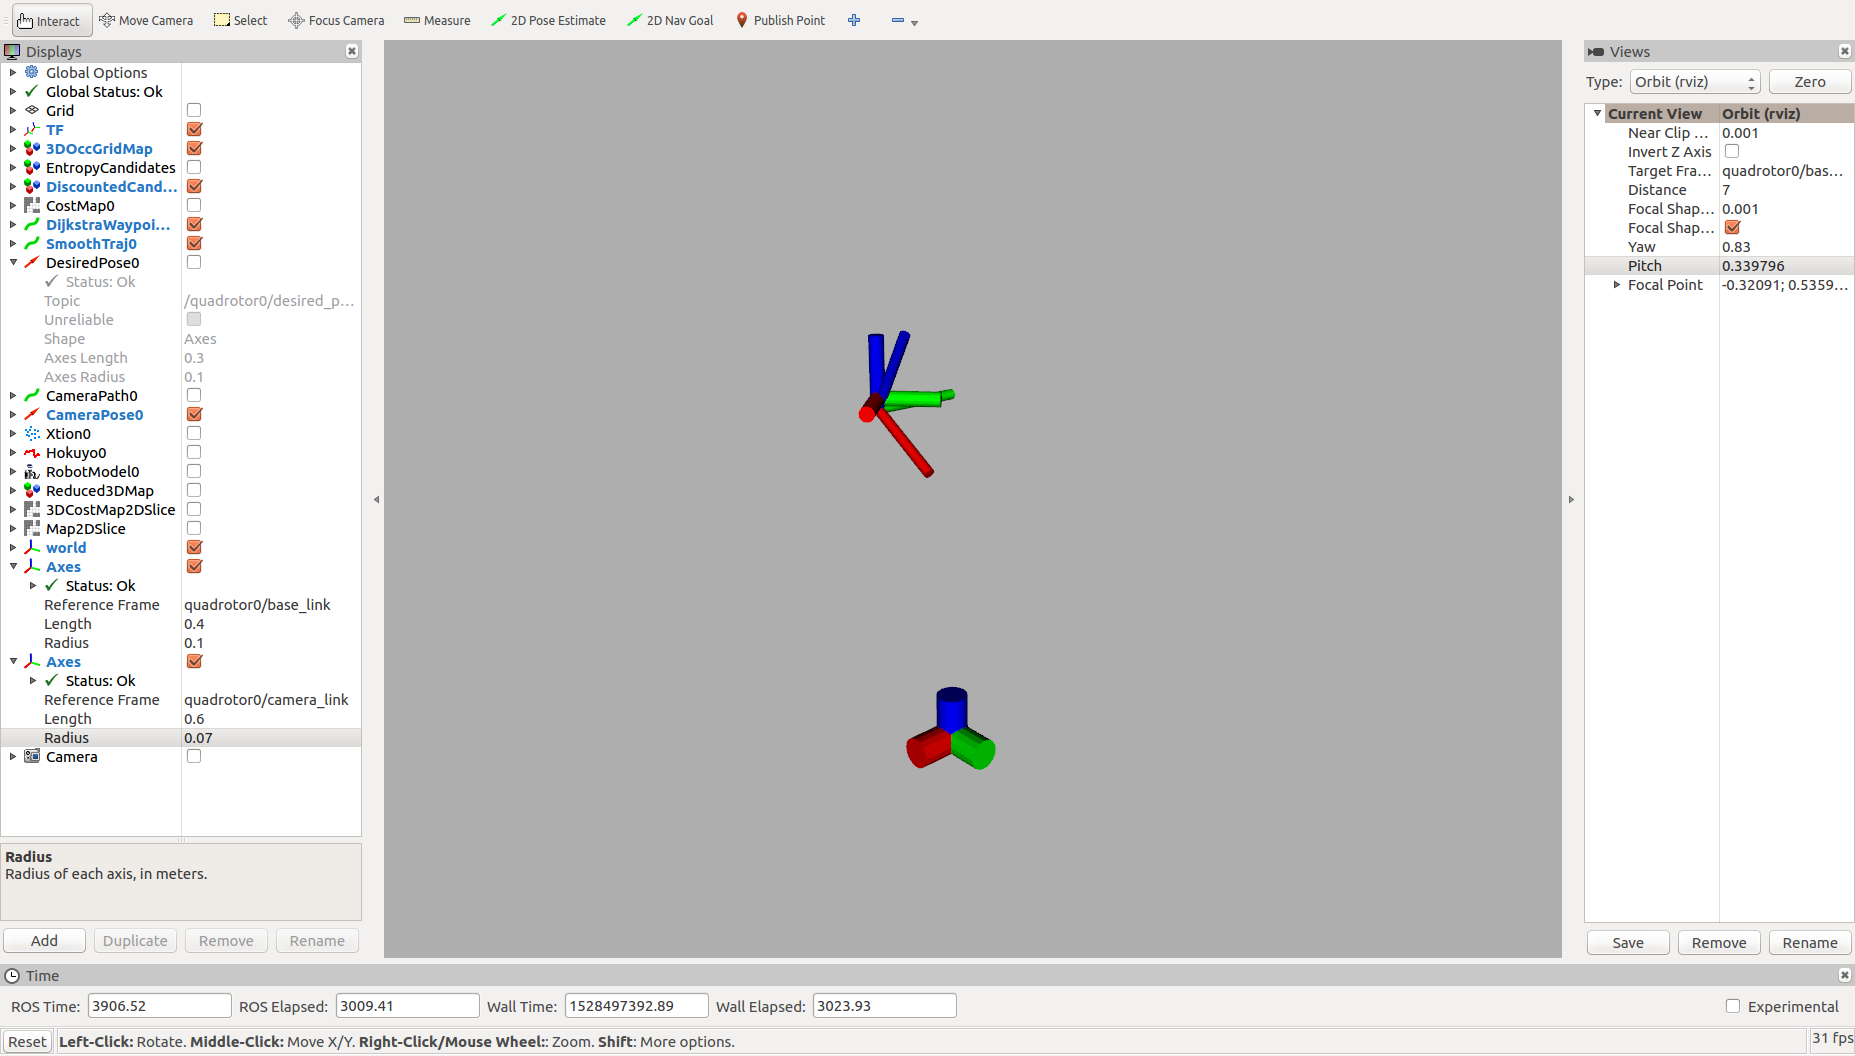
\includegraphics[trim = {21cm 5cm 20cm 5cm}, clip, height=1.0\textwidth]{mars_general.png}
        		\caption{General View}
    	\end{subfigure}
    	\begin{subfigure}[t]{0.3\columnwidth}
           	\centering
          	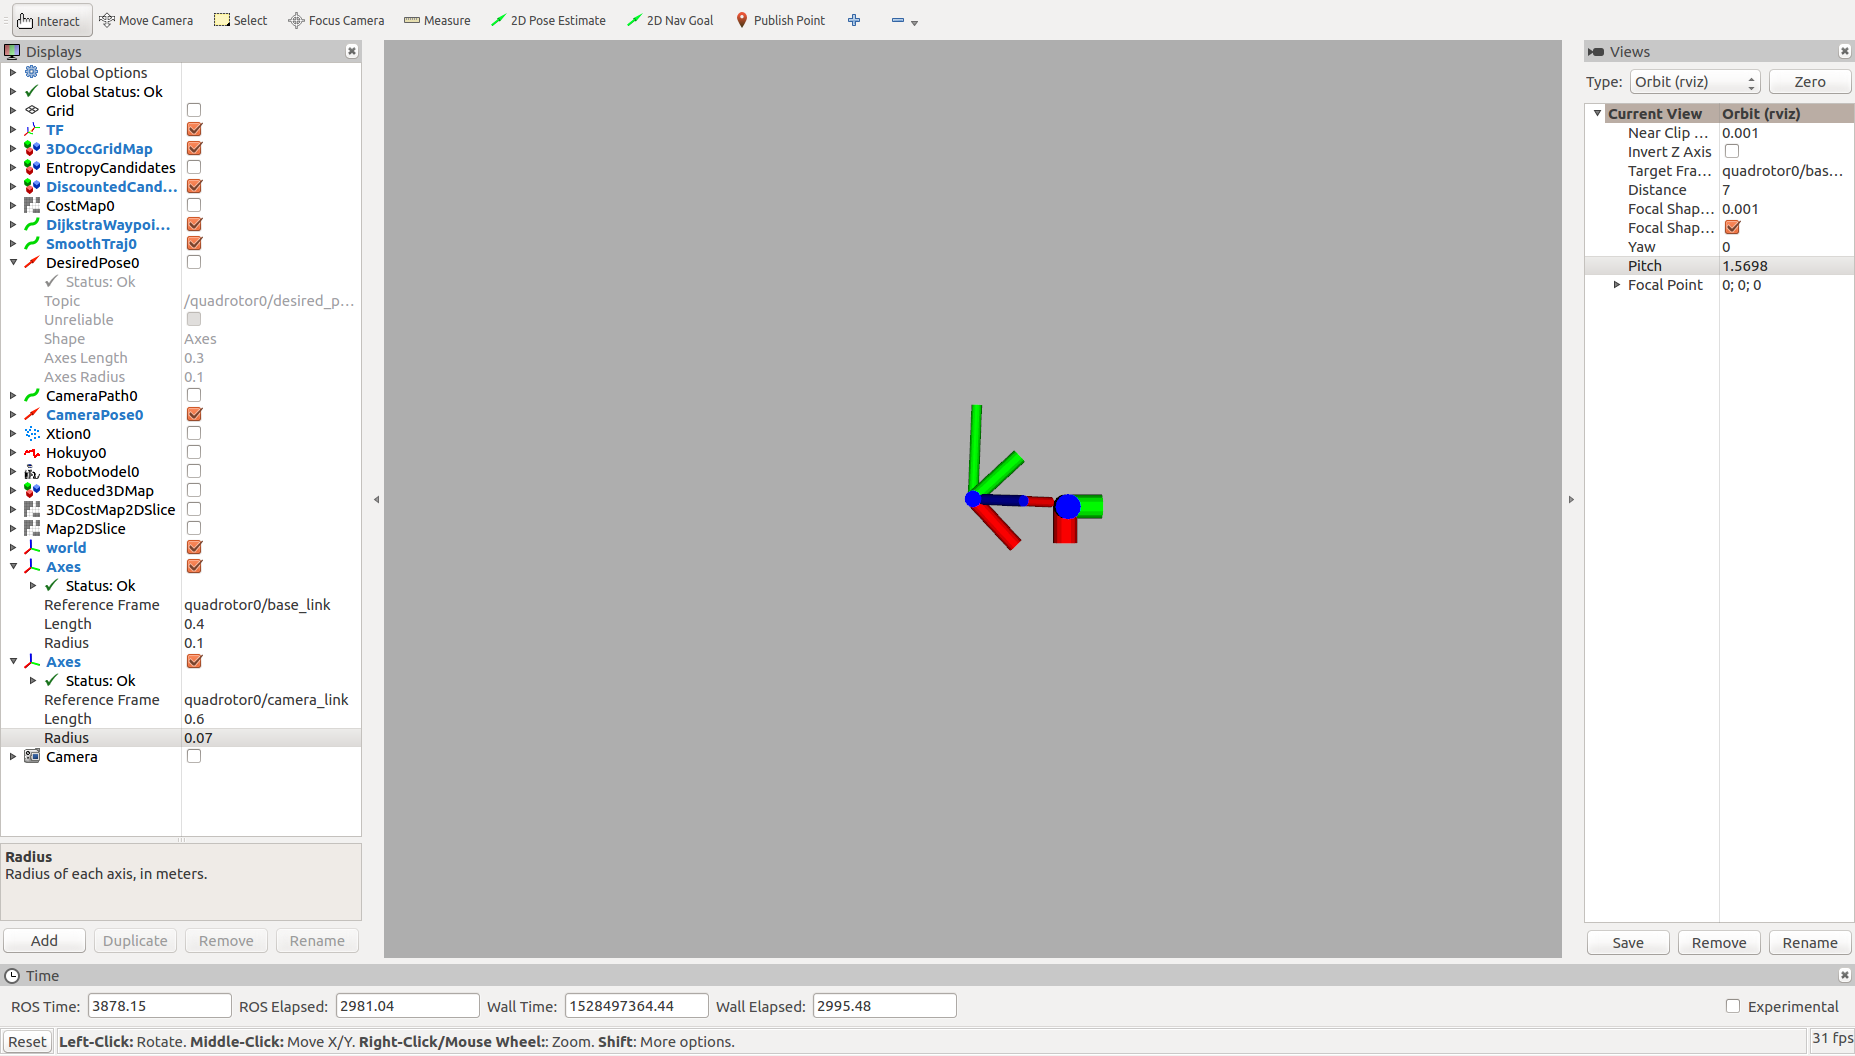
\includegraphics[trim = {25cm 6cm 16cm 4cm}, clip, height=1.0\textwidth]{mars_psi.png}
        		\caption{$\psi$ Rotation}
    	\end{subfigure}
	\begin{subfigure}[t]{0.3\columnwidth}
           	\centering
          	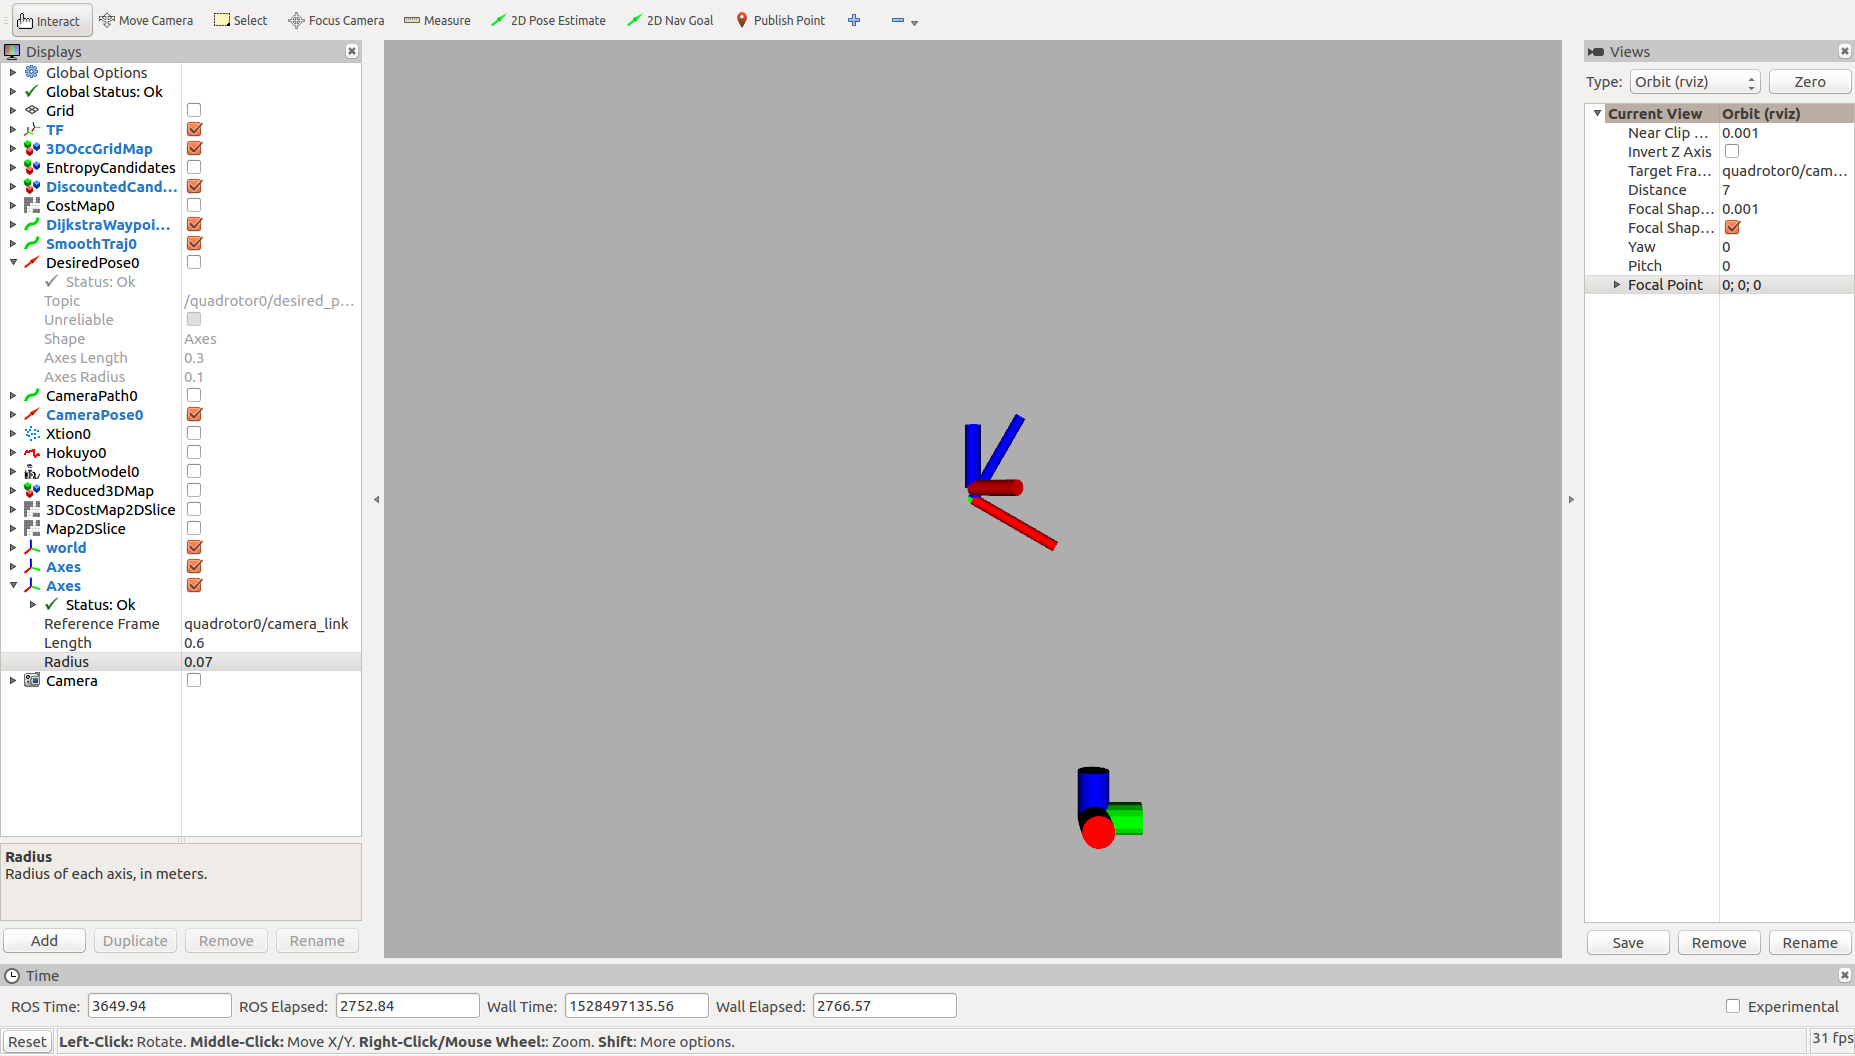
\includegraphics[trim = {23cm 4cm 17cm 6cm}, clip, height=1.0\textwidth]{mars_theta.png}
        		\caption{$\theta$ Rotation}
    	\end{subfigure}
%\includegraphics[width=2.5in]{myfigure}
% where an .eps filename suffix will be assumed under latex, 
% and a .pdf suffix will be assumed for pdflatex; or what has been declared
% via \DeclareGraphicsExtensions.
\caption{The three frames are shown with three axes (red: first axis, green: second axis, blue: third axis). The Mars frame (short and thick) is fixed to the planet. The body-fixed frame (medium thickness and length) is fixed to the camera frame (long and narrow). The rotation of $\psi$ (b) represents the fixed camera yaw rotation and $\theta$ (c) represents the downward angle of the camera to capture the surface of Mars below the flying robot.}
\label{fig:transforms}
\end{figure}


Next, we show how multiple 3D measurements provide an estimate for information gain. Let $\Psi$ and $\Theta$ be the angular ranges for sensor field-of-view (FOV) in the horizontal and vertical directions, respectively. Within the sensor FOV, we select sample measurements for evaluating their expected information gains. Let the number of sample measurements be $n_\psi$ and $n_\theta$ for horizontal and vertical rotations, respectively. Since $R_c$ and the FOV are known, the set of sample measurement rays, namely $\mathcal{Z}(R_c)$, is known as well. Then, the expected information gain for a single measurement ray $z$ from candidate position $x_c$ and attitude $R_c$ is the negative expected entropy change,
\begin{align}
\label{eqn:Iray}
\mathcal{I}_\text{ray}(x_c,R_c,\psi,\theta)=
\begin{cases}
H(P(r))-\text{E}[H(P(r|x_c,z(\psi+\tilde{\psi},\theta+\tilde{\theta})))], & \mbox{if } z(\psi+\tilde{\psi},\theta+\tilde{\theta})\in\mathcal{Z}(R_c), \\ 
0,                                                                                    & \mbox{otherwise},
\end{cases}
\end{align}
<<<<<<< HEAD
where the mounting yaw $\tilde{\psi}$ and pitch $\tilde{\theta}$ of the sensor is a fixed rotation in the horizontal and vertical directions, respectively in that order, such that $-\pi<\tilde{\psi}\leq\pi$ and $-\frac{\pi}{2}\leq\tilde{\theta}\leq\frac{\pi}{2}$. A positive $\tilde{\theta}$ corresponds to rotating the depth sensor from forward to downward toward the surface of Mars. The expected information gain for the full scan is the summation of expected information gains for individual rays
=======
where the mounting yaw $\tilde{\psi}$ and pitch $\tilde{\theta}$ of the sensor is a fixed rotation in the horizontal and vertical directions, respectively in that order, such that $-\pi<\tilde{\psi}\leq\pi$ and $-\frac{\pi}{2}+\frac\Theta2\leq\tilde{\theta}\leq\frac{\pi}{2}-\frac\Theta2$. A positive $\tilde{\theta}$ corresponds to rotating the depth sensor from a forward direction to a downward direction toward the surface of Mars. The expected information gain for the full scan is the summation of expected information gains for individual rays
>>>>>>> evan
\begin{align}
\label{eqn:Iscan}
\mathcal{I}_\text{scan}(x_c,R_c)=\sum_{i_\psi=1}^{n_\psi}\sum_{i_\theta=1}^{n_\theta}\mathcal{I}_\text{ray}\left(x_c,R_c,\frac{(2i_\psi-n_\psi-1)\Psi}{2n_\psi},\frac{(2i_\theta-n_\theta-1)\Theta}{2n_\theta}\right).
\end{align}

Finally, \refeqn{Iscan} is computed for $n_\psi$ possible attitudes when the robot is at location $x_c$, one corresponding to each yaw angle $\psi$. Then, the optimal attitude at $x_c$ is
\begin{align}
\label{eqn:RcStar}
R_c^*=\argmax_{R_c} \mathcal{I}_\text{scan}(x_c,R_c).
\end{align}

In short, the expected information gain from each possible measurement ray is obtained using predicted entropy from \refeqn{DiscExpEntropyRay} and \refeqn{ProbMeas}. Then the expected information gain from all possible scans at a candidate location is calculated from \refeqn{Iray} and \refeqn{Iscan}. Finally, the optimal attitude at this candidate location is found using \refeqn{RcStar}.

\subsection{Collision-Free Trajectory in 3D}

Next, we present a fairly straightforward application of Dijkstra's search to 3D occupancy grid mapping. First we reduced the number of grid cells to cubic blocks large enough for a robot to fit completely inside. Based on the occupancy probability of these blocks and their neighbors, we determine which cells are reachable, and what are their travel costs by building a cost map based on Dijkstra's algorithm.

Here we describe how a reduced map is generated for collision avoidance and motion planning. If the largest edge-to-edge distance of the robot, namely $\rho$, is not larger than the 3D grid cell size $\alpha$, this step is unnecessary. Let $k\geq1$ be an integer such that $k\alpha\geq\rho$ and $(k-1)\alpha<\rho$, i.e., $k$ is the minimum number of grid cells in each dimension capable of fully-enclosing the robot inside this cube. Then, we decompose the complete probabilistic 3D into map $ m_\text{reduced}$, which is composed of larger cubic cells that encompass $k^3$ cells from map $ m$. Let $\mathbf{m}_{\text{reduced},k}$ denote the $k$-th cell of $ m_\text{reduced}$ being occupied, and let $a_k\subset m$ be those $k^3$ cells from $ m$ composing this larger cell. Then, we apply an effective rule for collision-avoidance from~\cite{KauTakAiLee18} to obtain the probability of $\mathbf{m}_{\text{reduced},k}$,

\begin{align}
\label{eqn:Proj3DMapComb}
P(\mathbf{m}_{\text{reduced},k})= 
\begin{cases}
    \max_{i\in a_k}{P(\mathbf{m}_i)},	&\text{if} \ \max_{i\in a_k}{P(\mathbf{m}_i)}\geq P_\text{thresh},\\
    \min_{i\in a_k}{P(\mathbf{m}_i)},	& \text{otherwise},
\end{cases}
\end{align}
where initial probability is $0<P_\text{init}<1$ and the threshold probability is constrained to $P_\text{init}<P_\text{thresh}<1$. This approach uses probabilities that have changed from $P_\text{init}$, and favors occupied cells to avoid risking collisions.

<<<<<<< HEAD
Next, we show how $\mathbf{m}_{\text{reduced},k}$ is used in Dijkstra's search~\cite{Dij59}. Defining $0<P_\text{coll}<1$ as the acceptable probability of collision, every grid cell of $ m_\text{reduced}$ is considered a safe and unvisited node if its occupancy probability, and the occupancy probabilities of its neighbors (sharing a face, edge, or corner), are below $P_\text{coll}$. A cost map is built from the starting robot location by neighboring nodes, where the cost to travel to another node is based on Euclidian distance: a cell sharing a face is $\alpha$ away, a cell sharing an edge is $\sqrt2\alpha$ away, and a cell sharing a corner is $\sqrt3\alpha$ away. Generating a cost map for all reachable cells in $\mathbf{m}_{\text{reduced},k}$ provides a collision-free travel cost for all reachable candidate pose locations. Once an optimal pose is selected, the path is easily found from the cost map using steepest descent.
=======
Next, we show how $\mathbf{m}_{\text{reduced},k}$ is used in Dijkstra's search~\cite{Dij59} for collision avoidance and motion planning. Defining $0<P_\text{coll}<1$ as the acceptable probability of collision, every grid cell of $ m_\text{reduced}$ is considered a safe and unvisited node if its occupancy probability, and the occupancy probabilities of its neighbors (sharing a face, edge, or corner), are below $P_\text{coll}$. A cost map is built from the starting robot location by neighboring nodes, where the cost to travel to another node is based on Euclidian distance: a cell sharing a face is $\alpha$ away, a cell sharing an edge is $\sqrt2\alpha$ away, and a cell sharing a corner is $\sqrt3\alpha$ away. Generating a cost map for all reachable cells in $\mathbf{m}_{\text{reduced},k}$ provides a collision-free travel cost for all reachable candidate pose locations. Once an optimal pose is selected, the path is easily found from the cost map using steepest descent.
>>>>>>> evan


\subsection{Optimal 3D Pose}

Here we present how an optimal pose is selected based on information gains at optimal attitudes and known collision-free travel costs. First, we show a function to account for travel costs, and then we account for these costs inside the optimization.

The proposed autonomous exploration follows a receding-horizon framework, meaning that optimal poses and trajectories are computed as quickly as possible, even if the robot has not reached the prior optimal pose. However, the computation is not instantaneous; let the distance $d_\text{opt}$ denote the distance that the robot can travel between optimal pose updates. Then, we define a \emph{bump function} loosely based on~\cite{Joh06}, defined as
\begin{align}
\label{eqn:BumpFunRecedingHorizon}
\mathcal B(d)=
\begin{cases}
f_\text{max},												& \text{if }0\leq d\leq d_\text{opt}
\\
(f_\text{max}-f_\text{far})\exp\braces{-\beta(d_\text{opt}-d)^2}+f_\text{far},	& \text{if }d>d_\text{opt}
\end{cases},
\end{align}
where $d$ is a travel distance along the cost map, $f_\text{max}>f_\text{far}>0$, and $\beta>0$ is an exponential decay rate of the bump, which is illustrated in Fig. \ref{fig:recedingHorizonBumpFun}. The main idea is that when travel costs are low, the bump function is large, but the bump decreases with increasing travel cost.

	\begin{figure}
	\vspace*{-0.3\columnwidth}
		\centerline{
			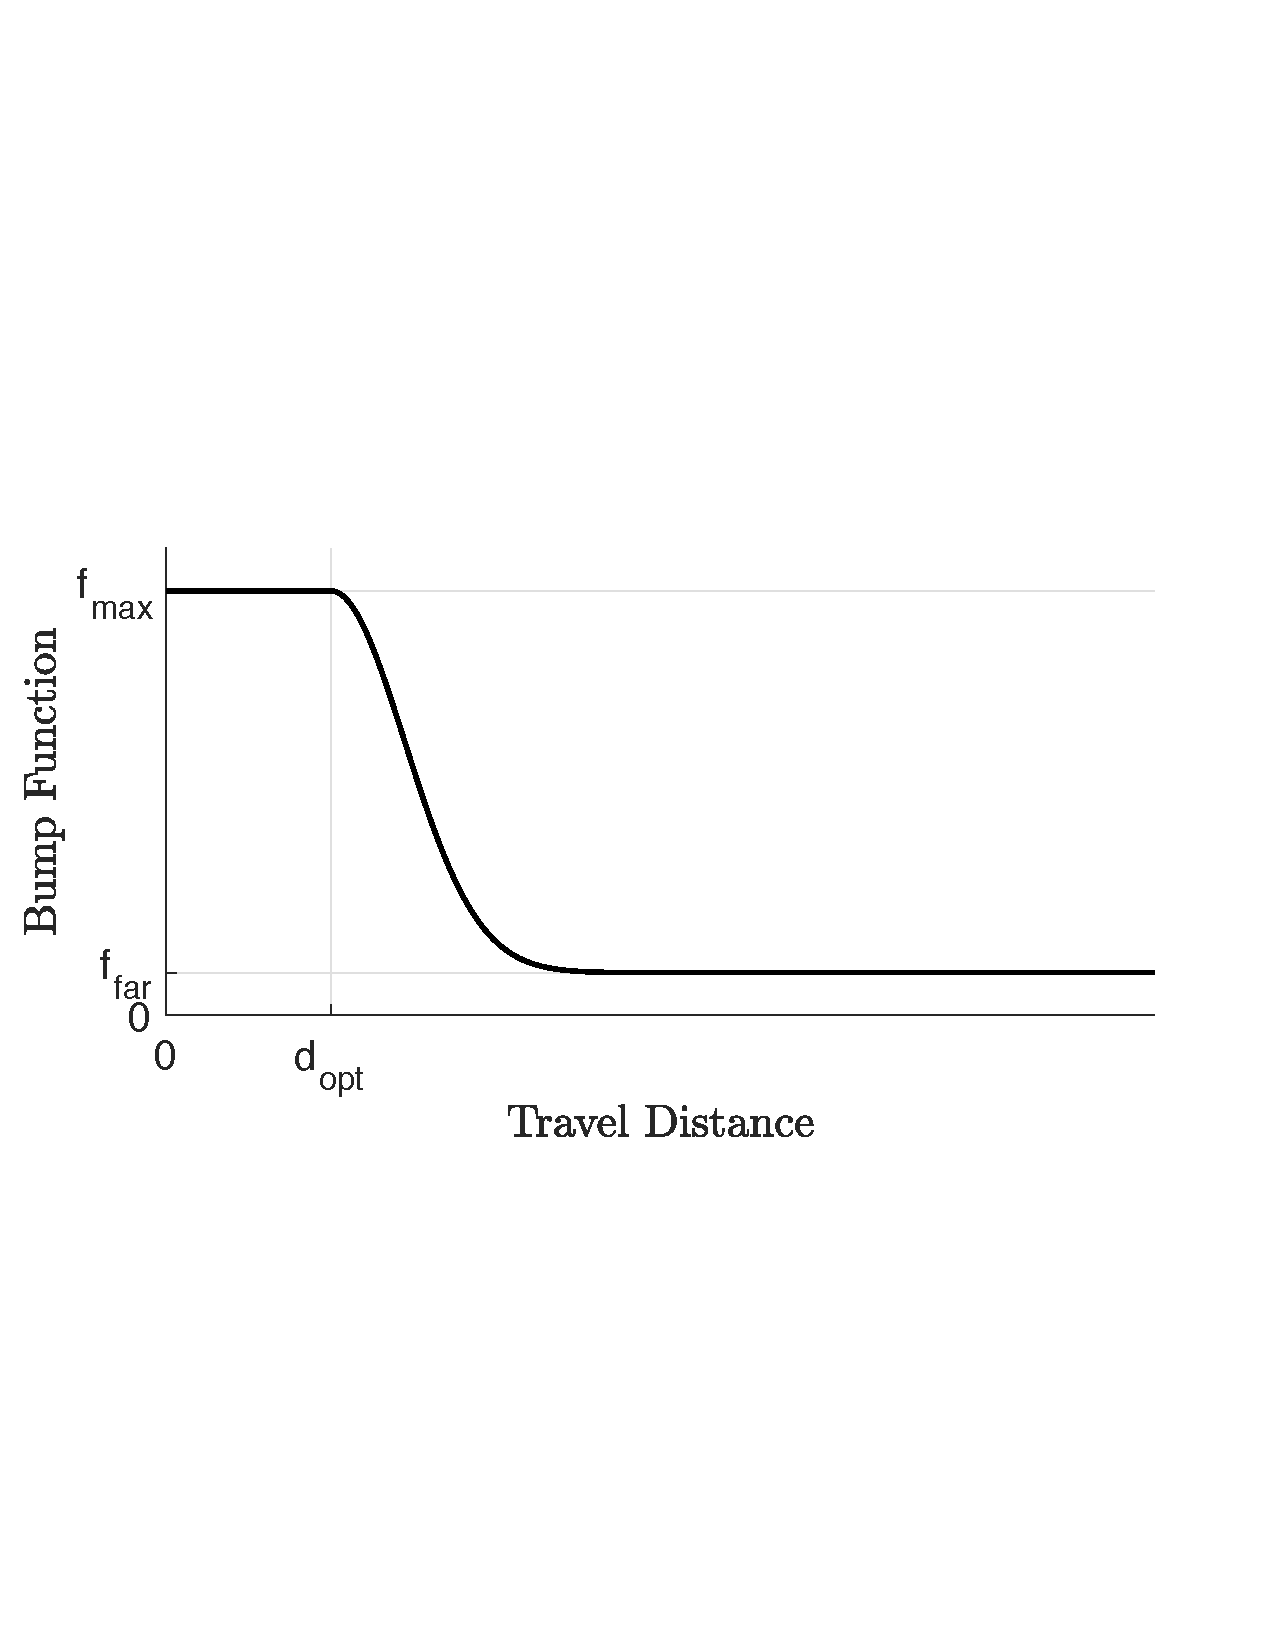
\includegraphics[width=0.6\columnwidth]{recedingHorizonBumpFunFlattened.pdf}
		}
	\vspace*{-0.25\columnwidth}
		\caption{The bump function is multiplied to the objective function of \refeqn{CandidateLocationOptimization} to prioritize local trajectories to avoid traversals across the map, where travel costs are determined using Dijkstra's algorithm. However, there is no time wasted up to $d_\text{opt}$ because this distance may be achieved in the minimum exploration computation time.}
		\label{fig:recedingHorizonBumpFun}
	\end{figure}

Finally, we incorporate expected information gain and travel costs into a unified optimization. Given $d(x_c)$ from Dijkstra's cost map, the optimal candidate location is
\begin{align}
\label{eqn:CandidateLocationOptimization}
x_c^*=\argmax_{x_c}\mathcal{I}_\text{scan}(x_c,R_c^*)\mathcal B(d(x_c)),
\end{align}
and therefore the optimal pose is $X_c^*=\braces{x_c^*,R_c^*}$.

In conclusion, every reachable candidate pose is considered for its optimal attitude. The travel costs, acquired from Dijkstra's search, serve as input for the bump function, which prioritizes local trajectories to avoid costly map traversals. Then, the optimal candidate location is selected to maximize a combination of expected information gain and travel cost.


%\begin{itemize}
%	\item Describe the entropy calculation of expected information gain of all ray combinations is computationally intractable
%	\item Proposed strategy: multiple rays in 3D, and optimal attitude covers the rays with the greatest summation of information gains
%	\item Dijkstra's search in 3D, polynomial trajectories
%	\item Complete optimization
%	\item Concluding paragraph
%\end{itemize}


\section{Numerical Examples}
\label{sec:NumExamples}

In this section, we demonstrate the efficacy of the proposed 3D mapping and autonomous exploration with a simulated Mars environment. First we cover the software structure and parameters, then compare results using two different maps for entropy prediction.


\subsection{Software}

<<<<<<< HEAD
The mapping, exploration, and visualization processes communicate over the Robot Operating System (ROS) framework (Kinetic distribution), and Gazebo 8 serves as the simulator for the physical objects and measurements. There are two major programs, referred to as \emph{nodes} in ROS, used during the simulation: mapping and exploration. The mapping node takes measurements from a 3D laser scanner and pairs those with the sensor transformation relative to Mars using the ROS Transform Message Filters package. Then, it builds a 3D probabilistic map using \refeqn{RayISMAnswer}-\refeqn{Unnormalized}. The mapping node sends updates from the probabilistic map to the exploration node, which decomposes the full map $m$ into $ m_\text{reduced}$ according to \refeqn{Proj3DMapComb}, and builds a cost map based on Dijkstra's search to determine collision-free trajectory costs for all pose candidates. Finally, it applies \refeqn{RcStar}, \refeqn{BumpFunRecedingHorizon}, and \refeqn{CandidateLocationOptimization} to update the desired robot trajectory on a receding-horizon. An overview of the process is illustrated in Fig. \ref{fig:NodesDiagram}.
=======
The mapping, exploration, and visualization processes communicate over the Robot Operating System (ROS) framework (Kinetic distribution), and Gazebo 8 serves as the simulator for the physical objects and measurements. There are two major programs, referred to as \emph{nodes} in ROS, used during the simulation: mapping and exploration. The mapping node takes measurements from a 3D laser scanner and pairs those with the sensor transformation relative to Mars using the ROS Transform Message Filters package. Then, it builds a 3D probabilistic map using ray casting and the inverse sensor model \refeqn{RayISMAnswer}-\refeqn{Unnormalized}. The mapping node sends updates from the probabilistic map to the exploration node, which decomposes the full map $m$ into $ m_\text{reduced}$ according to \refeqn{Proj3DMapComb}, and builds a cost map based on Dijkstra's search to determine collision-free trajectory costs for all pose candidates. Finally, the exploration node applies \refeqn{RcStar}, \refeqn{BumpFunRecedingHorizon}, and \refeqn{CandidateLocationOptimization} to update the desired robot trajectory on a receding-horizon. An overview of the process is illustrated in Fig. \ref{fig:NodesDiagram}.
>>>>>>> evan

	\begin{figure}
		\centerline{
			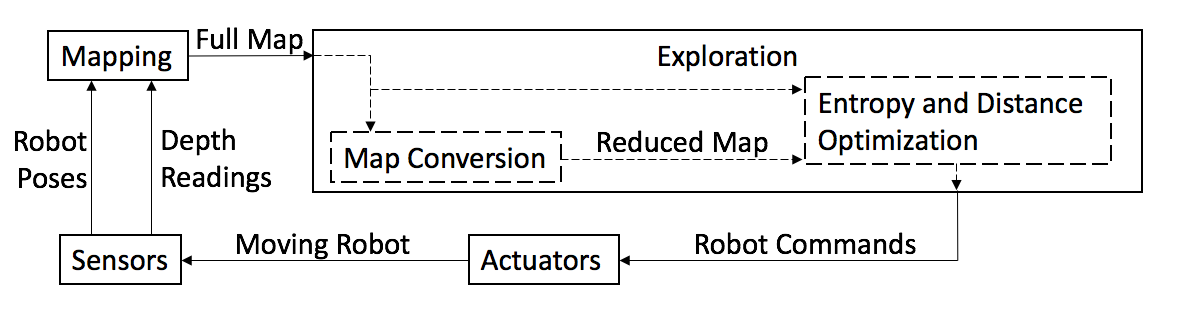
\includegraphics[width=0.8\columnwidth]{node_diagram_3D_mars.png}
		}
<<<<<<< HEAD
		\caption{The diagram of the 3D probabilistic mapping and autonomous exploration nodes shows the primary processes and communication lines.}
=======
		\caption{The diagram of the 3D probabilistic mapping and autonomous exploration nodes shows the primary processes and communication lines. These ROS nodes (boxes) operate together in real-time.}
>>>>>>> evan
		\label{fig:NodesDiagram}
	\end{figure}
	

\subsection{Results}

A 3D environment of Mars is simulated in Gazebo. A height map~\cite{mapaplanet} is used to generate a contoured surface, and the corresponding picture of Mars is draped over this contour, shown in Fig. \ref{fig:MarsGazebo}. A 3D laser scanner is also simulated in Gazebo. In the horizontal direction, the sensor has limits $\Psi=120\degree$ with a total of $1000$ measurement rays inside, the sensor is fixed at angle $\tilde{\psi}=45\degree$, and $n_\psi=16$ sample measurements are used. In the vertical direction, the sensor also has limits $\Theta=120\degree$ with a total of $1000$ measurement rays inside, but the sensor is fixed at angle $\tilde{\theta}=30\degree$, and $n_\psi=7$ sample measurements are used. These ray samples are taken from each candidate location, which are separated $1$ m apart in each of the $3$ dimensions.

% trim={<left> <lower> <right> <upper>}


\begin{figure}[!t]
	\centering
	\begin{subfigure}[t]{0.3\columnwidth}
           	\centering
          	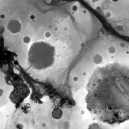
\includegraphics[height=0.9\textwidth]{mars_heightmap.png}
        		\caption{Height Map}
    	\end{subfigure}
    	\begin{subfigure}[t]{0.3\columnwidth}
           	\centering
          	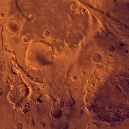
\includegraphics[height=0.9\textwidth]{mars_colormap.png}
        		\caption{Color Map}
    	\end{subfigure}
    	\begin{subfigure}[t]{0.3\columnwidth}
           	\centering{
<<<<<<< HEAD
          	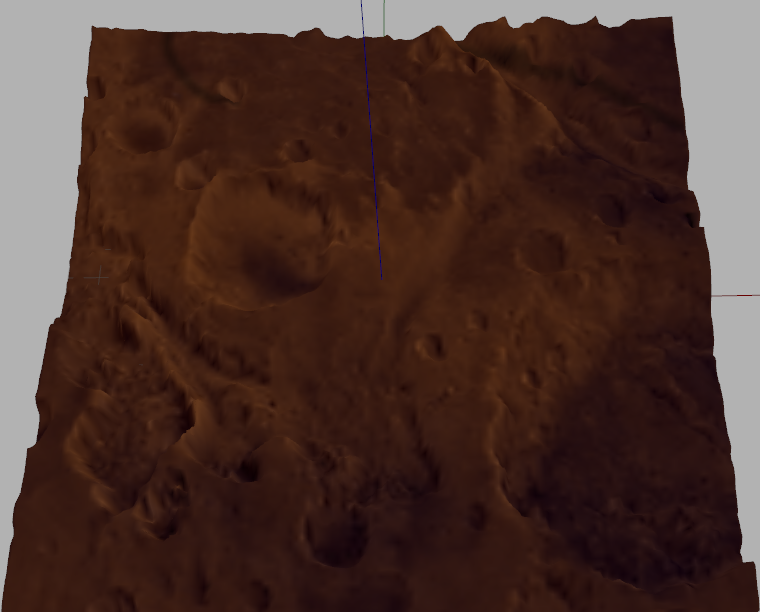
\includegraphics[height=0.9\textwidth]{mars_gazebo_sqr.png}}
        		\caption{Gazebo Environment}
    	\end{subfigure}
\caption{The height map (a) and color map (b) are used in Gazebo (c) to simulate a Mars environment.}
\label{fig:MarsGazebo}
\end{figure}

The map parameters are also important to the success of the exploration. The full map has dimensions $20$ m $\times$ $20$ m $\times$ $5$ m in the Mars-fixed frame, with cell edge length $\alpha=0.075$ m. The reduced map for collision-avoidance and motion planning has cells $k=3$ times the size ($0.225$ m), so $k^3=27$ cells are considered in \refeqn{Proj3DMapComb}. The bump functions use $f_\text{max}=1.0$, $f_\text{far}=0.1$, and $\beta=0.1$ to account for travel costs with \refeqn{BumpFunRecedingHorizon}. The receding horizon optimal time $d_\text{opt}$ is based on a fixed robot velocity of $0.25$ m/sec and the computation time varies from $0.6$ sec to $1.0$ sec.

The simulation was run twice. Case 1 was as described in this paper. Case 2 was identical to Case 1, except the reduced map $ m_\text{reduced}$ is used when computing \refeqn{Iscan}. Case 2 is largely inspired by the promising results of~\cite{KauTakAiLee18}, where a projected map based on the same criteria as \refeqn{Proj3DMapComb} proved effective for level flight. The resulting occupancy grid maps and complete map entropy are shown in Figs. \ref{fig:mars3Dogm} and \ref{fig:mars3Dentropy}, respectively.

\begin{figure}[!t]
	\centering
	\begin{subfigure}[t]{0.4\columnwidth}
           	\centering
          	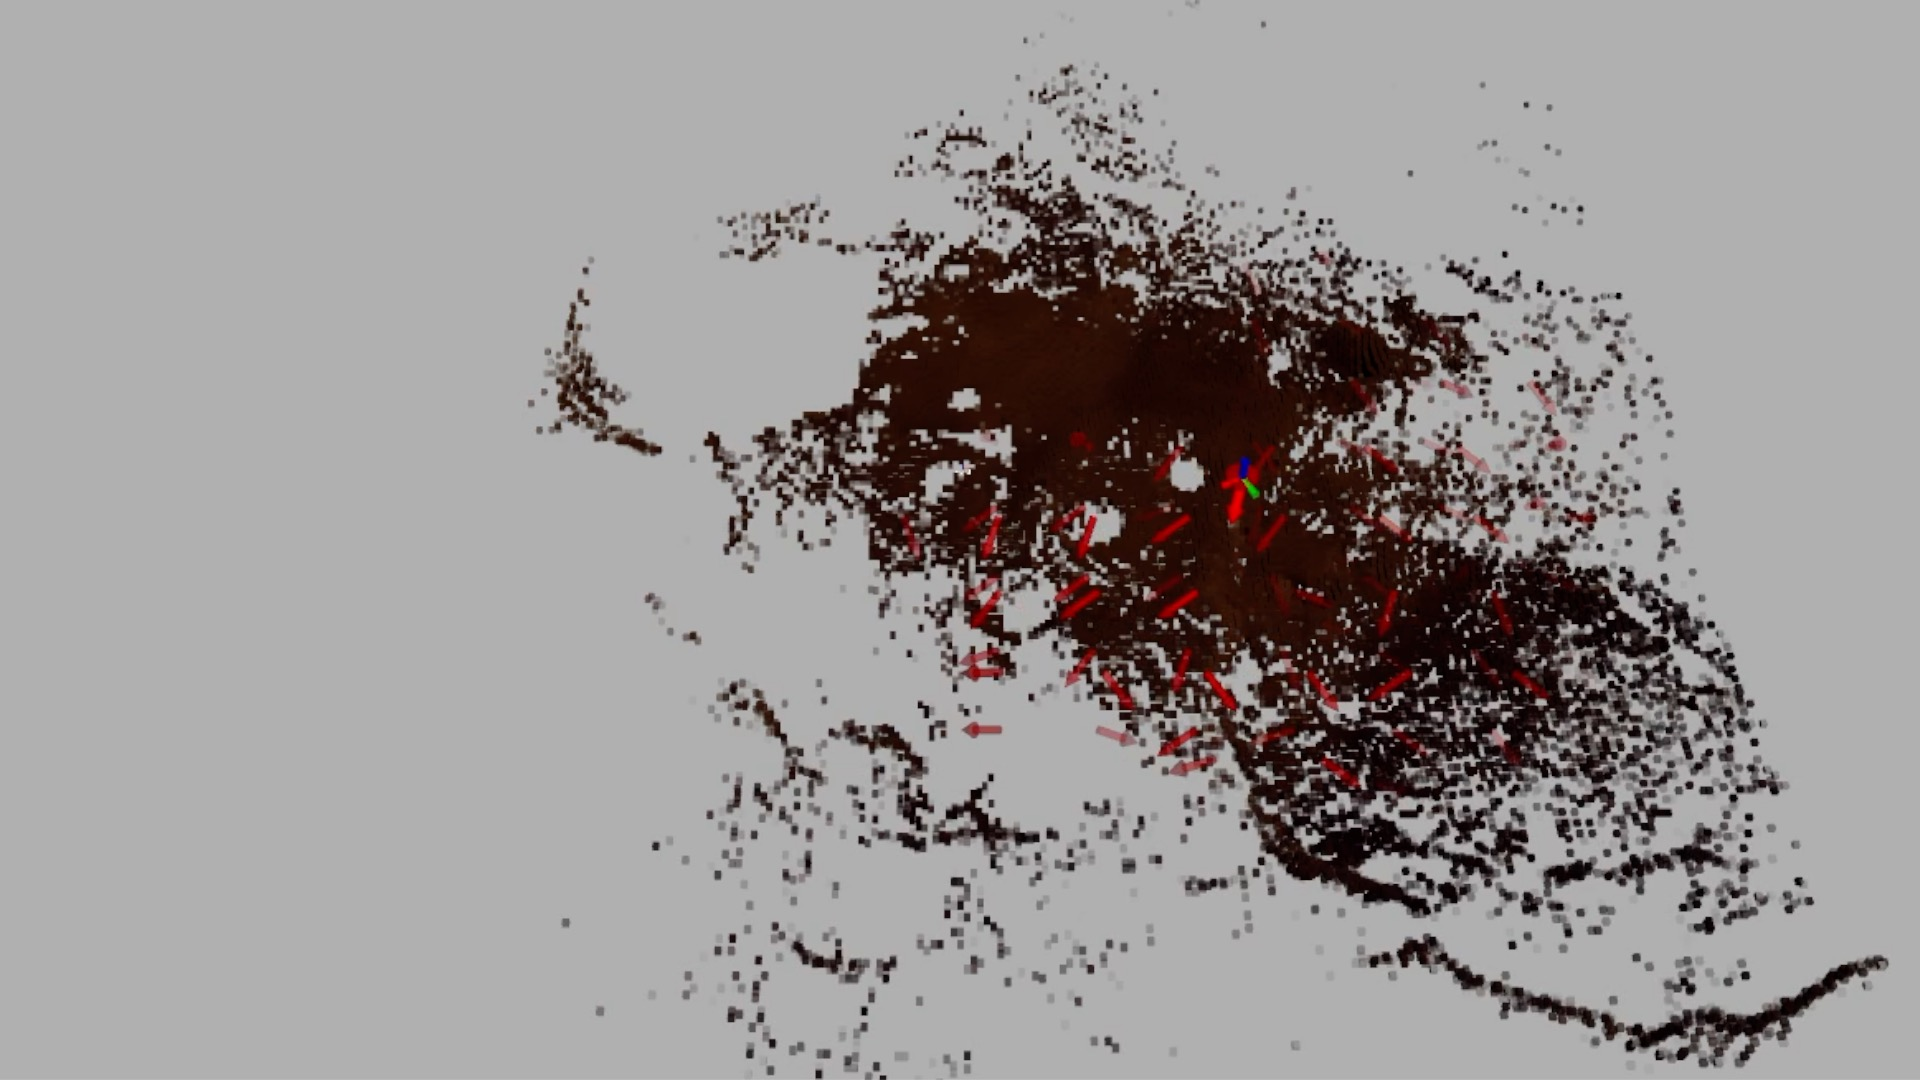
\includegraphics[height=0.5\textwidth]{MarsFullMap1min.jpg}
        		\caption{Case 1: $1$ min}
		\vspace*{0.025\textwidth}
    	\end{subfigure}
    	\begin{subfigure}[t]{0.4\columnwidth}
           	\centering
          	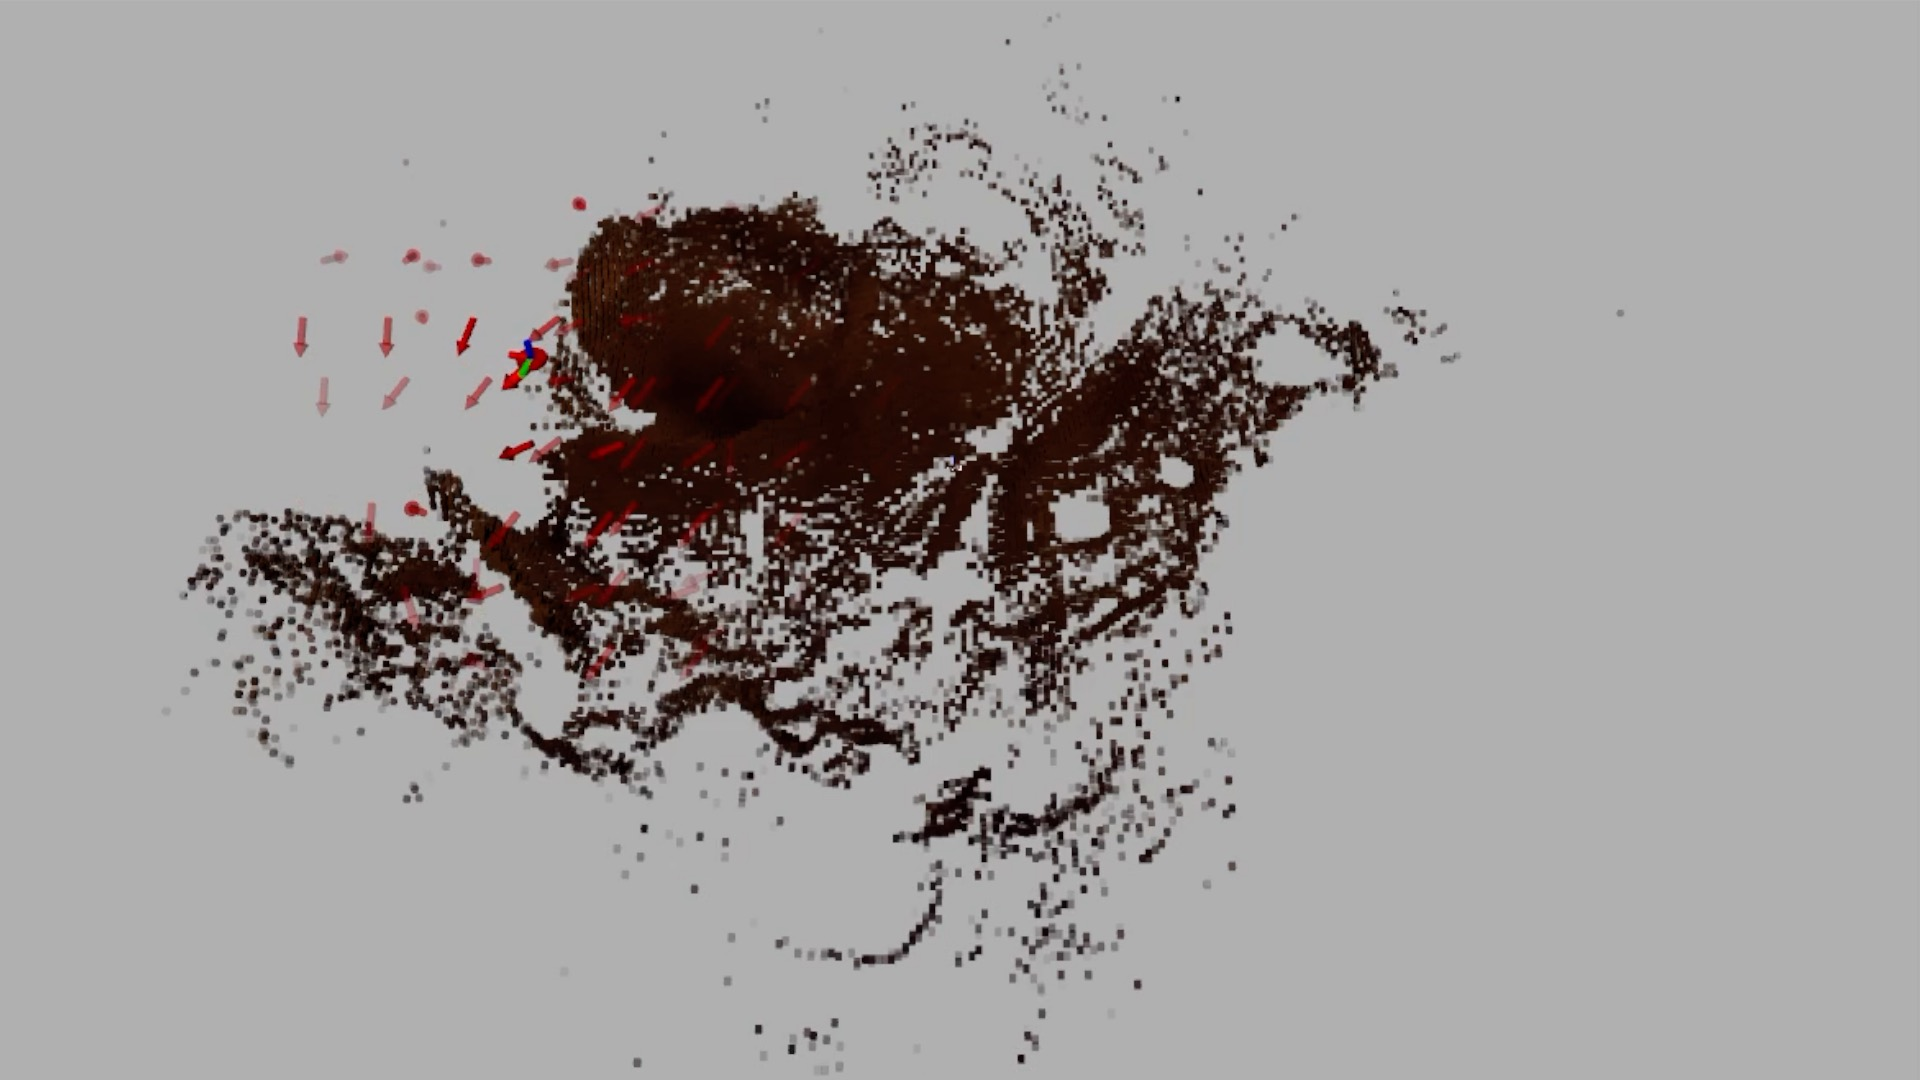
\includegraphics[height=0.5\textwidth]{MarsRdcdMap1min.jpg}
        		\caption{Case 2: $1$ min}
		\vspace*{0.025\textwidth}
    	\end{subfigure}
	\centering
	\begin{subfigure}[t]{0.4\columnwidth}
           	\centering
          	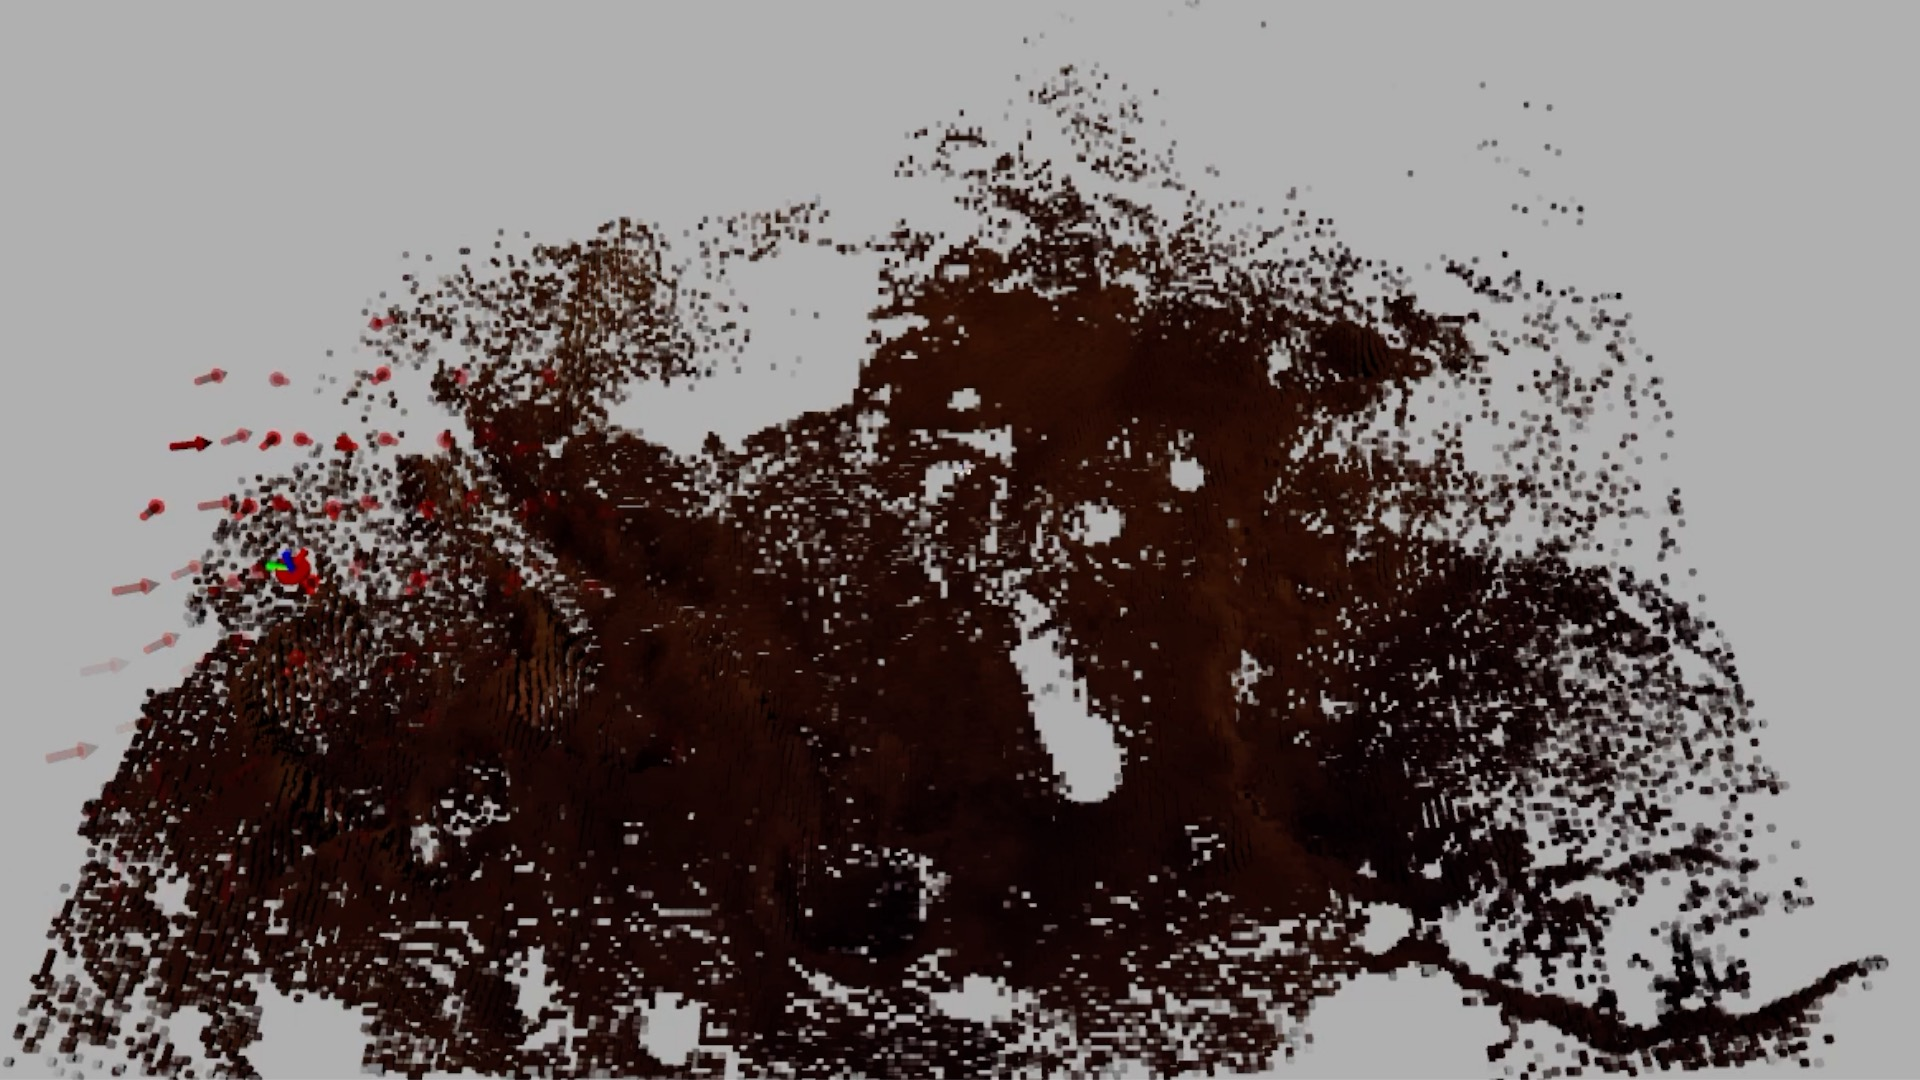
\includegraphics[height=0.5\textwidth]{MarsFullMap2min.jpg}
        		\caption{Case 1: $2$ min}
		\vspace*{0.025\textwidth}
    	\end{subfigure}
    	\begin{subfigure}[t]{0.4\columnwidth}
           	\centering
          	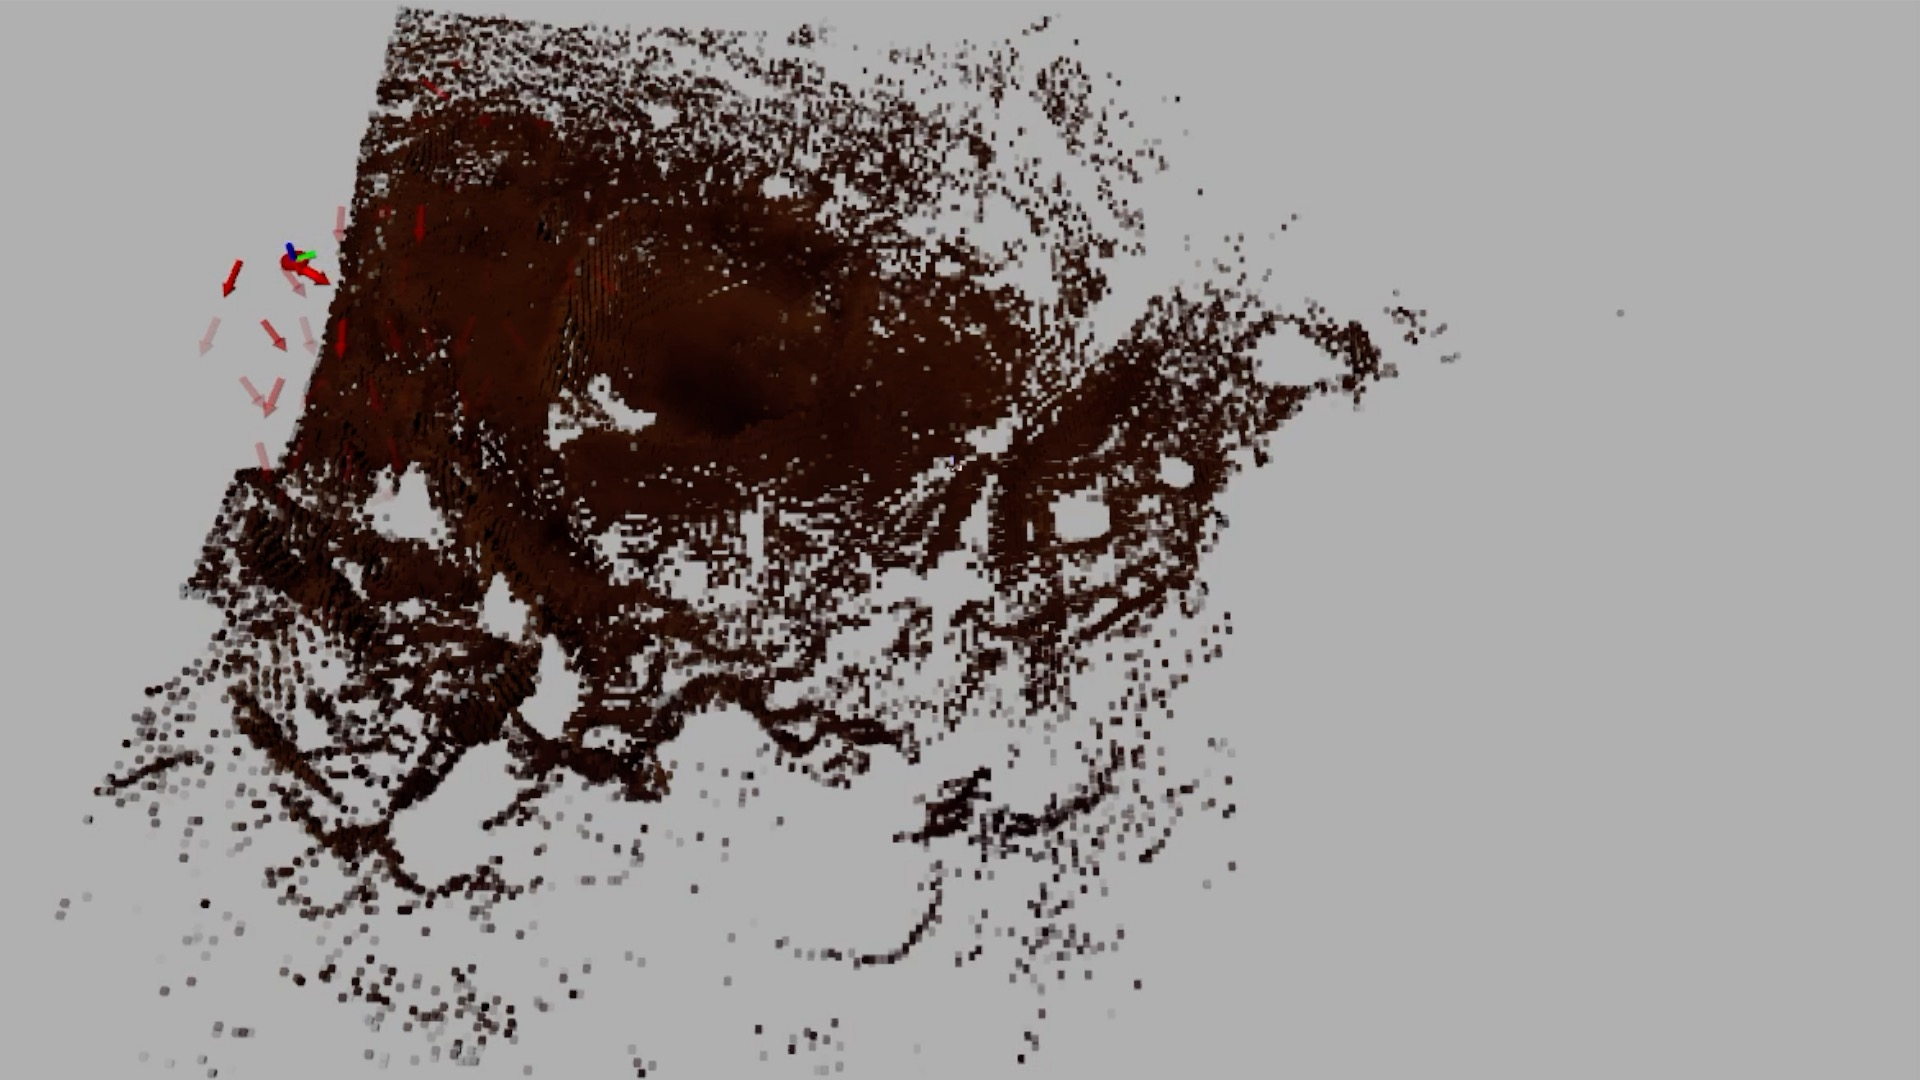
\includegraphics[height=0.5\textwidth]{MarsRdcdMap2min.jpg}
        		\caption{Case 2: $2$ min}
		\vspace*{0.025\textwidth}
    	\end{subfigure}
	\centering
	\begin{subfigure}[t]{0.4\columnwidth}
           	\centering
          	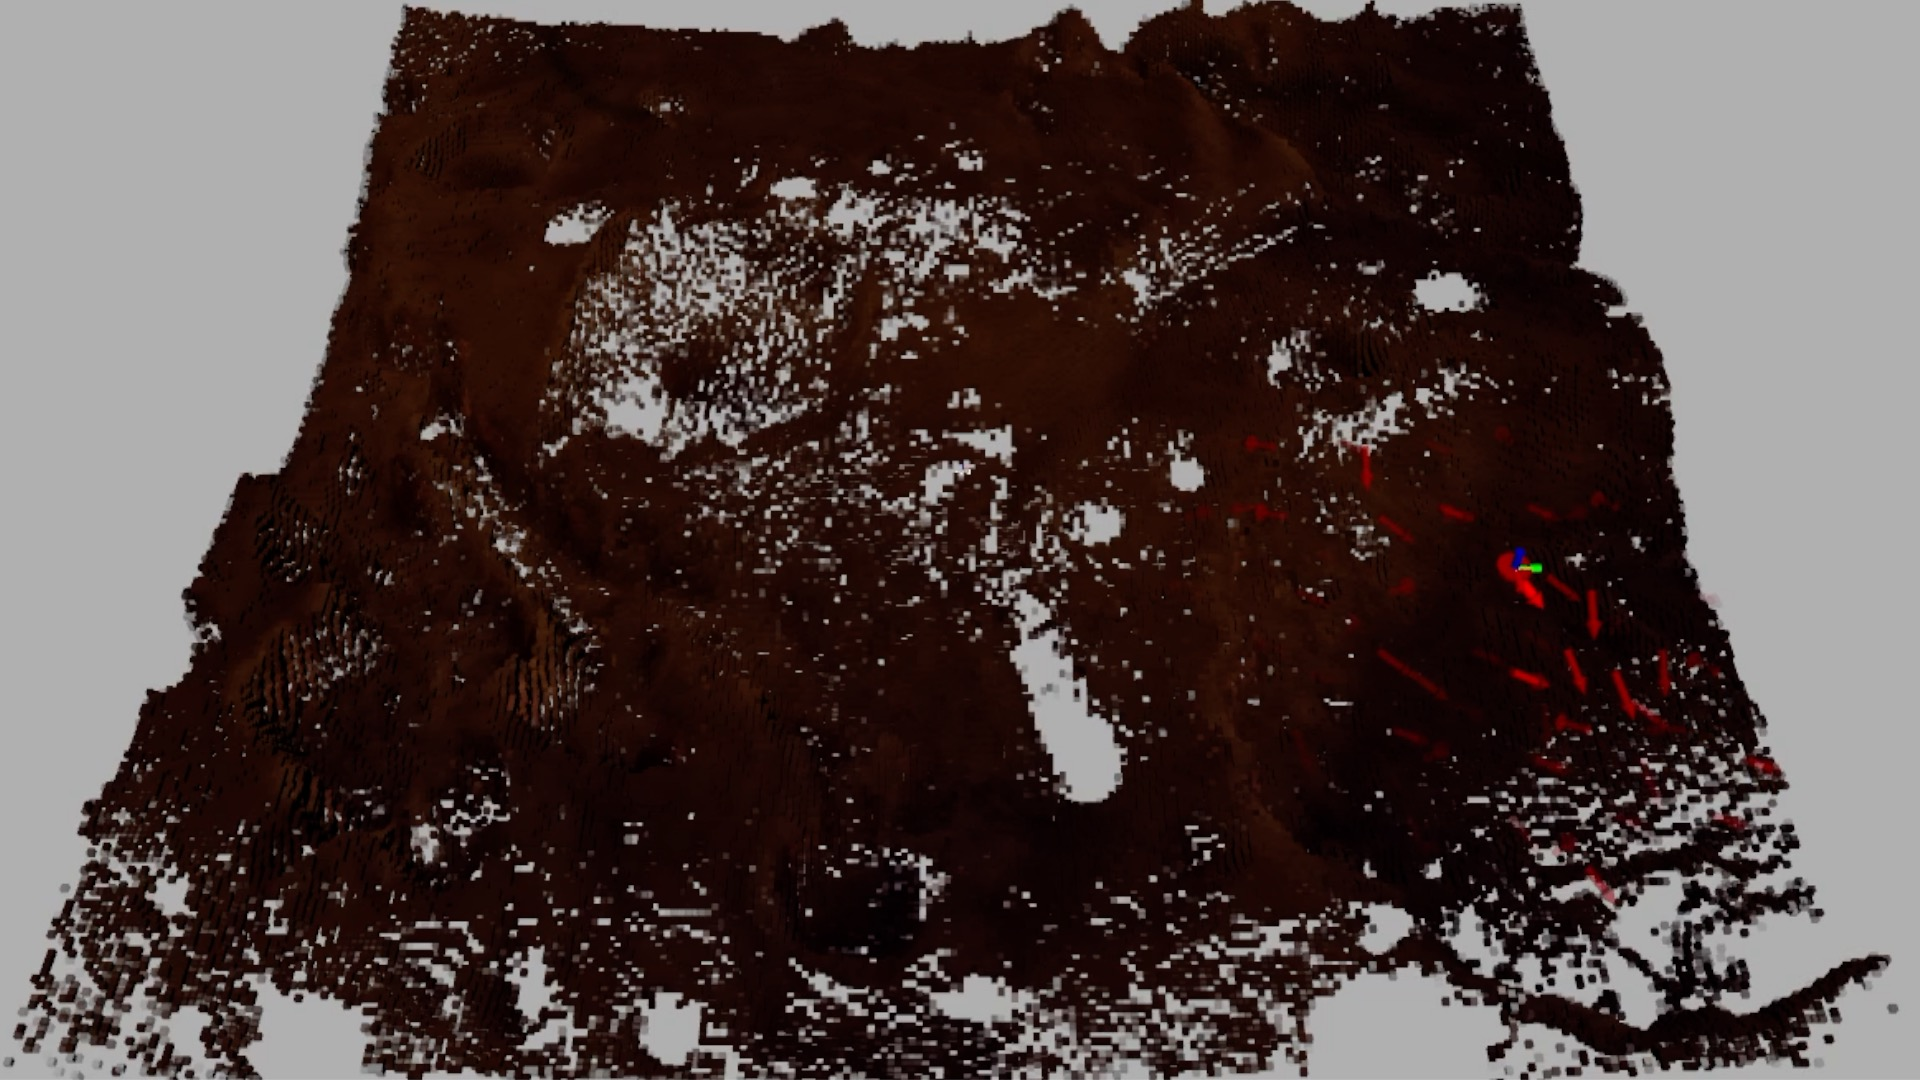
\includegraphics[height=0.5\textwidth]{MarsFullMap5min.jpg}
        		\caption{Case 1: $5$ min}
		\vspace*{0.025\textwidth}
    	\end{subfigure}
    	\begin{subfigure}[t]{0.4\columnwidth}
           	\centering
          	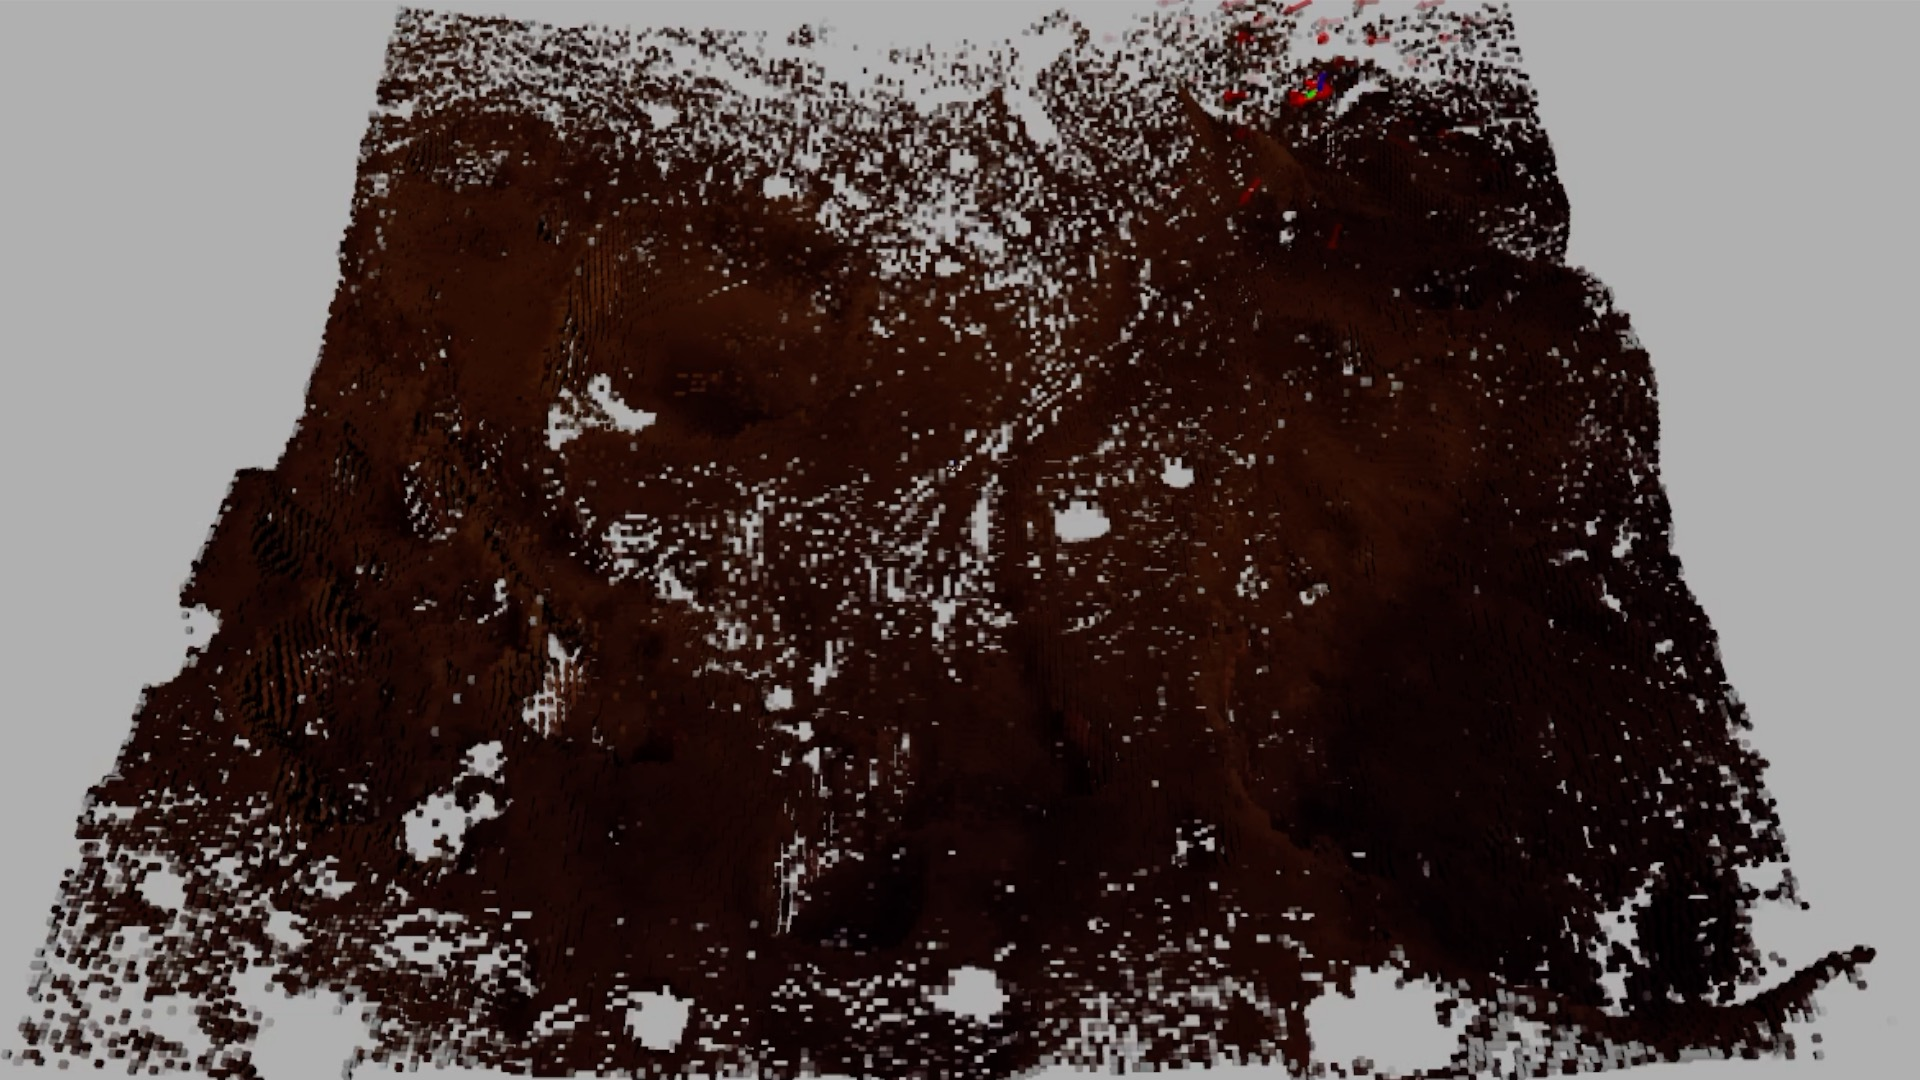
\includegraphics[height=0.5\textwidth]{MarsRdcdMap5min.jpg}
        		\caption{Case 2: $5$ min}
		\vspace*{0.025\textwidth}
    	\end{subfigure}
	\centering
	\begin{subfigure}[t]{0.4\columnwidth}
           	\centering
          	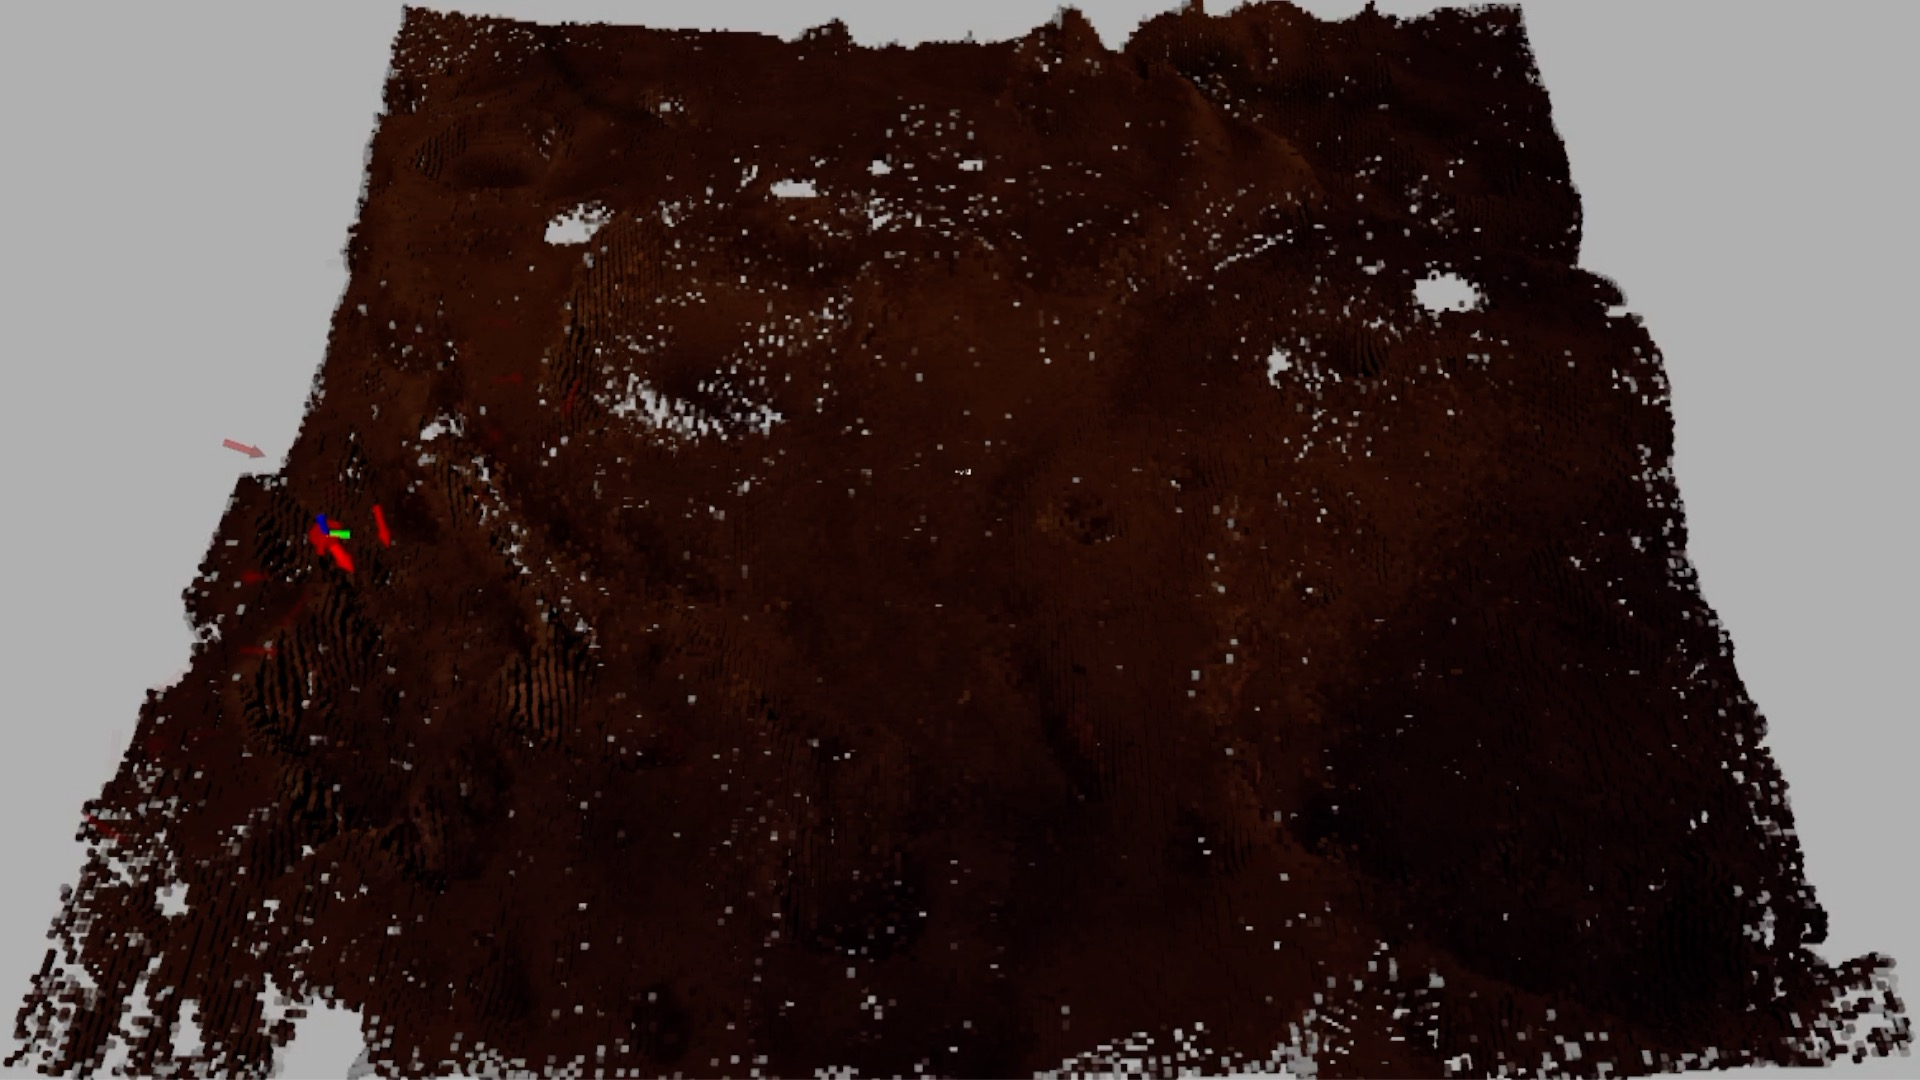
\includegraphics[height=0.5\textwidth]{MarsFullMap10min.jpg}
        		\caption{Case 1: $10$ min}
		\vspace*{0.025\textwidth}
    	\end{subfigure}
    	\begin{subfigure}[t]{0.4\columnwidth}
           	\centering
          	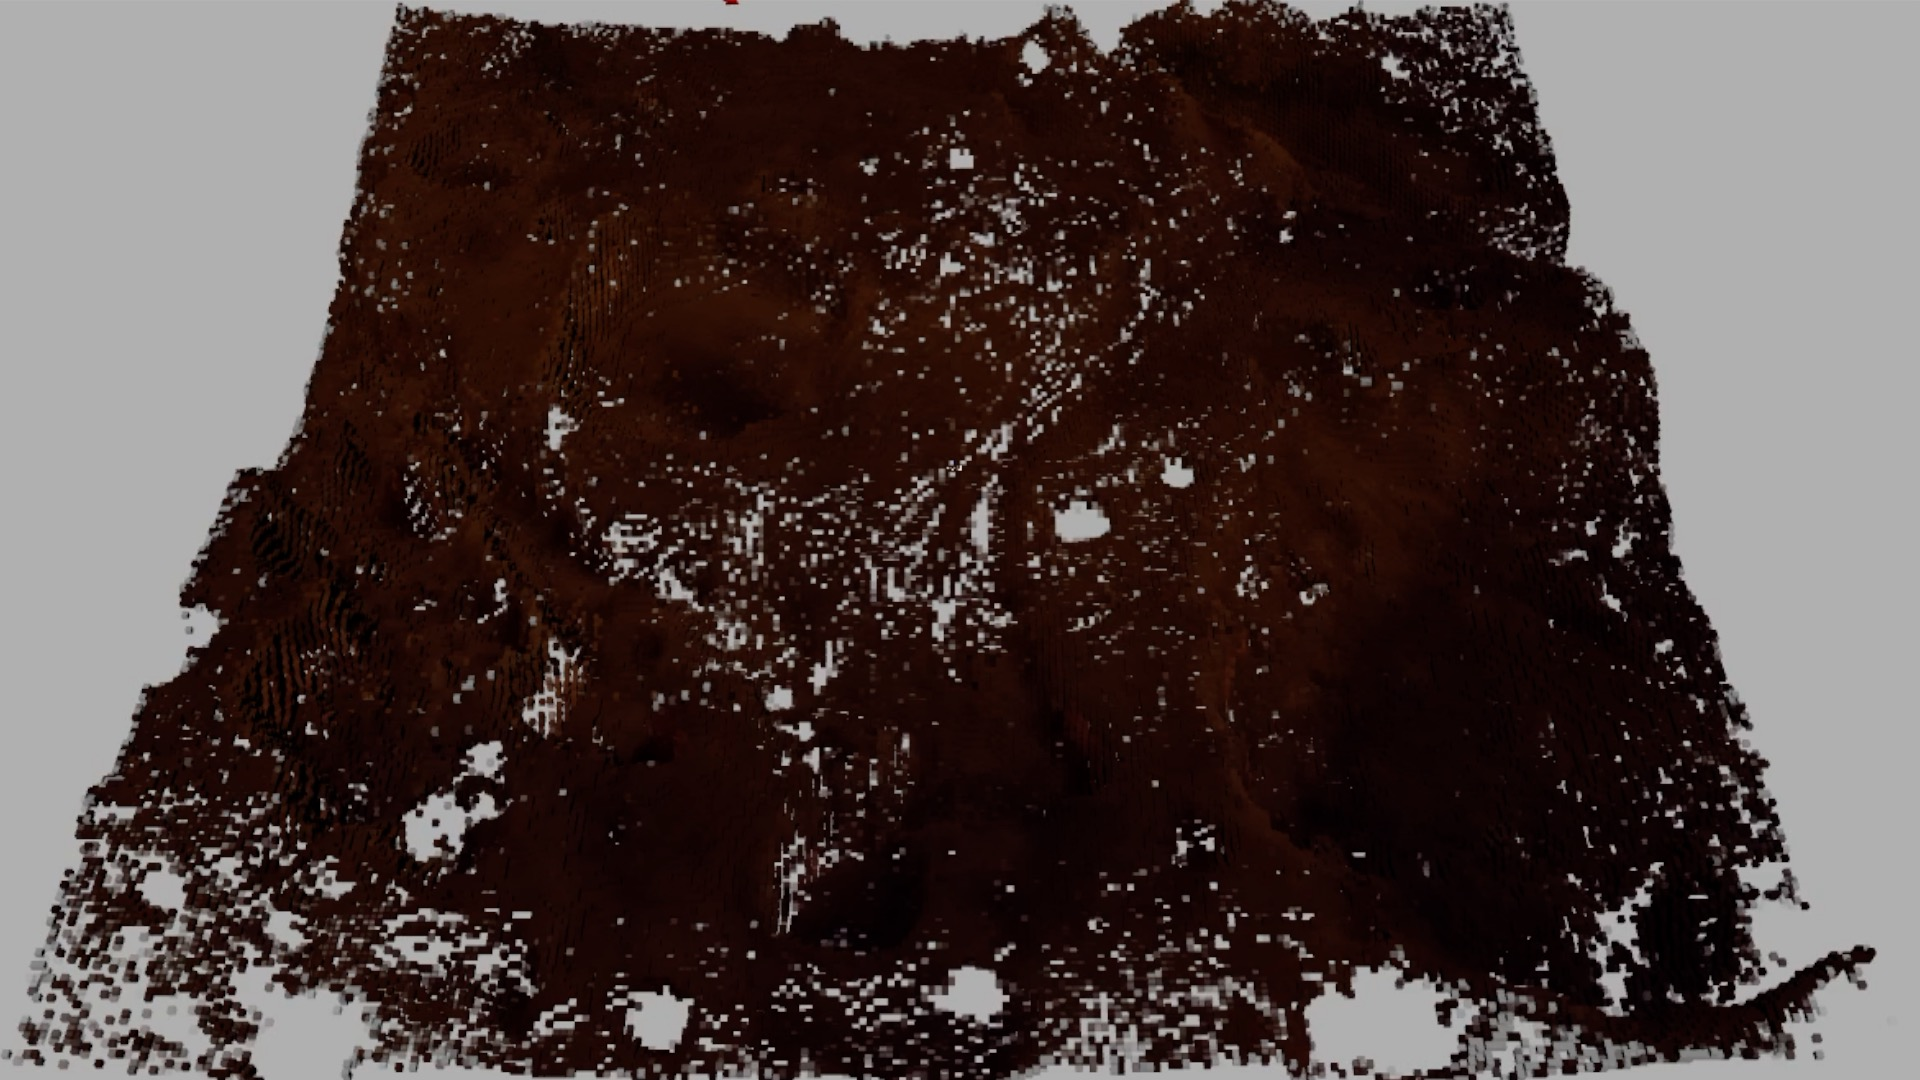
\includegraphics[height=0.5\textwidth]{MarsRdcdMap10min.jpg}
        		\caption{Case 2: $10$ min}
		\vspace*{0.025\textwidth}
    	\end{subfigure}
	\centering
	\begin{subfigure}[t]{0.4\columnwidth}
           	\centering
          	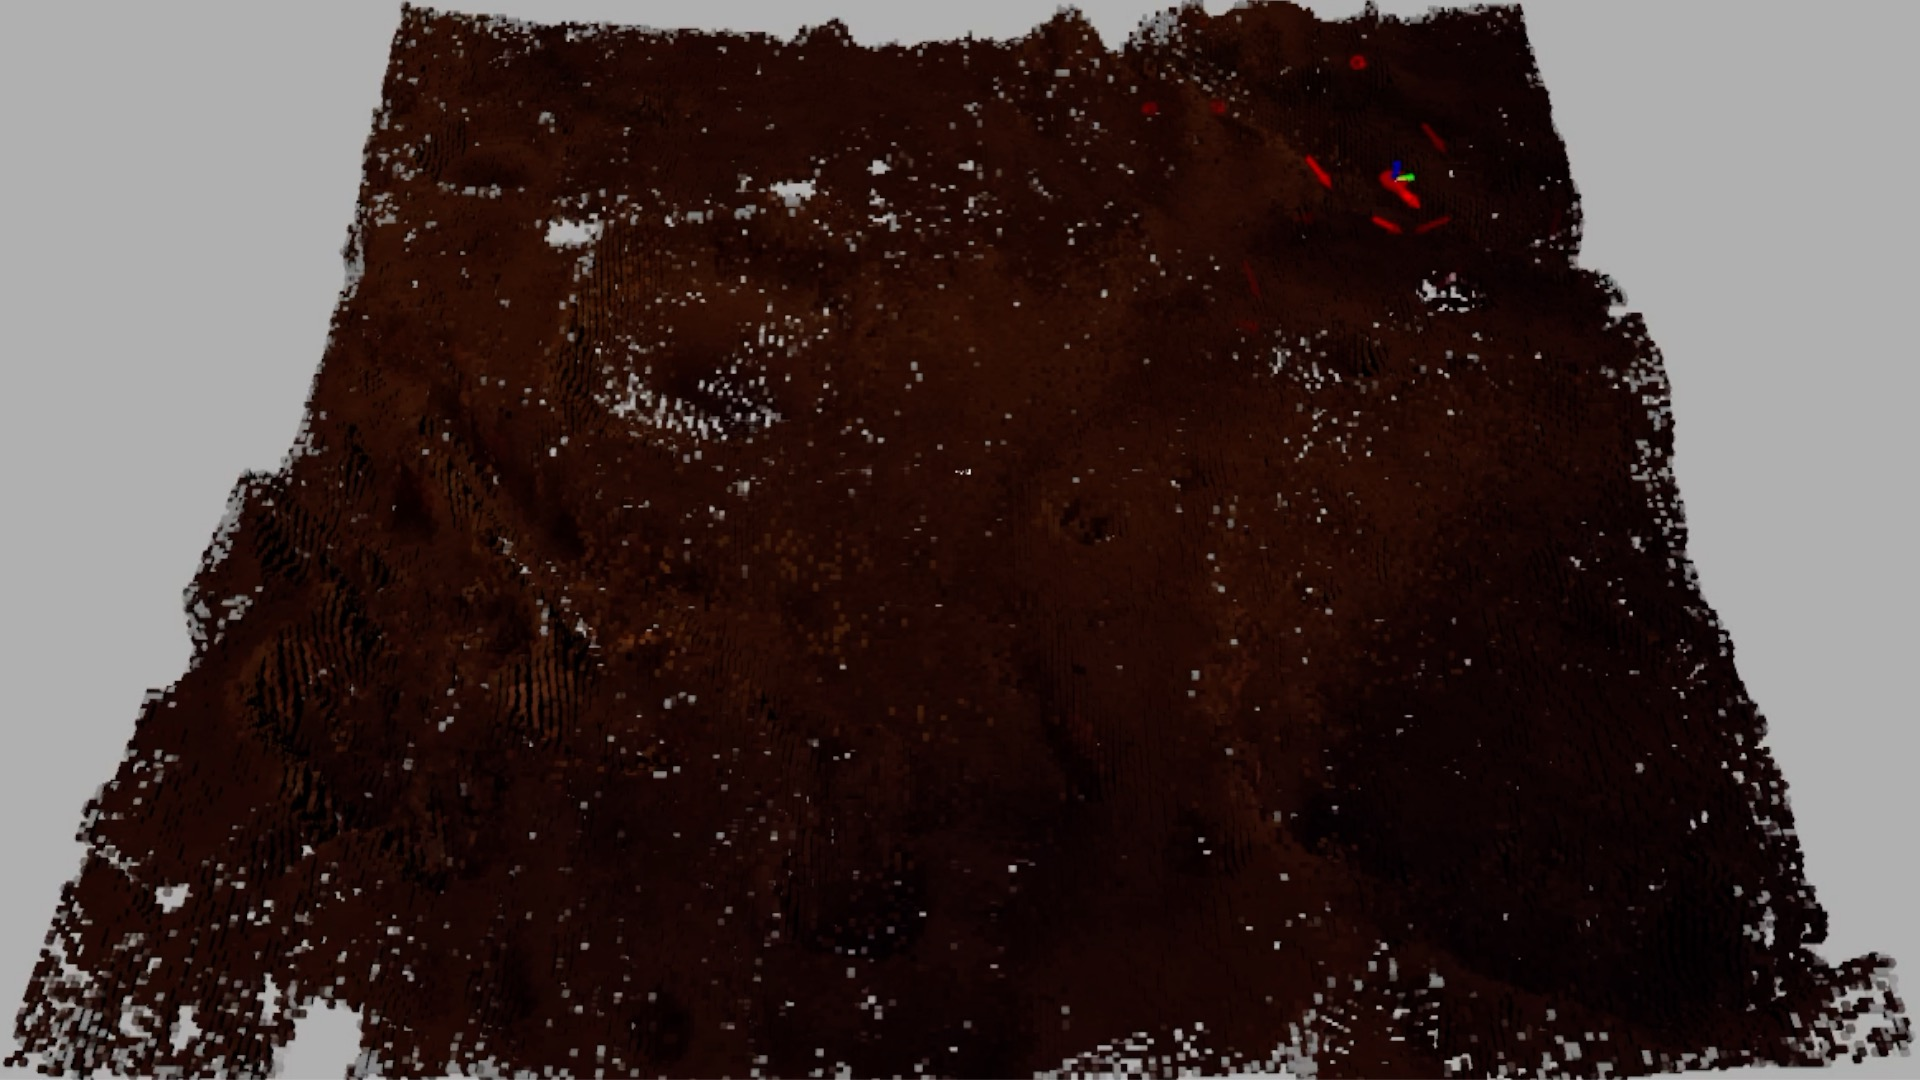
\includegraphics[height=0.5\textwidth]{MarsFullMap15min.jpg}
        		\caption{Case 1: $15$ min}
		\vspace*{0.025\textwidth}
    	\end{subfigure}
    	\begin{subfigure}[t]{0.4\columnwidth}
           	\centering
          	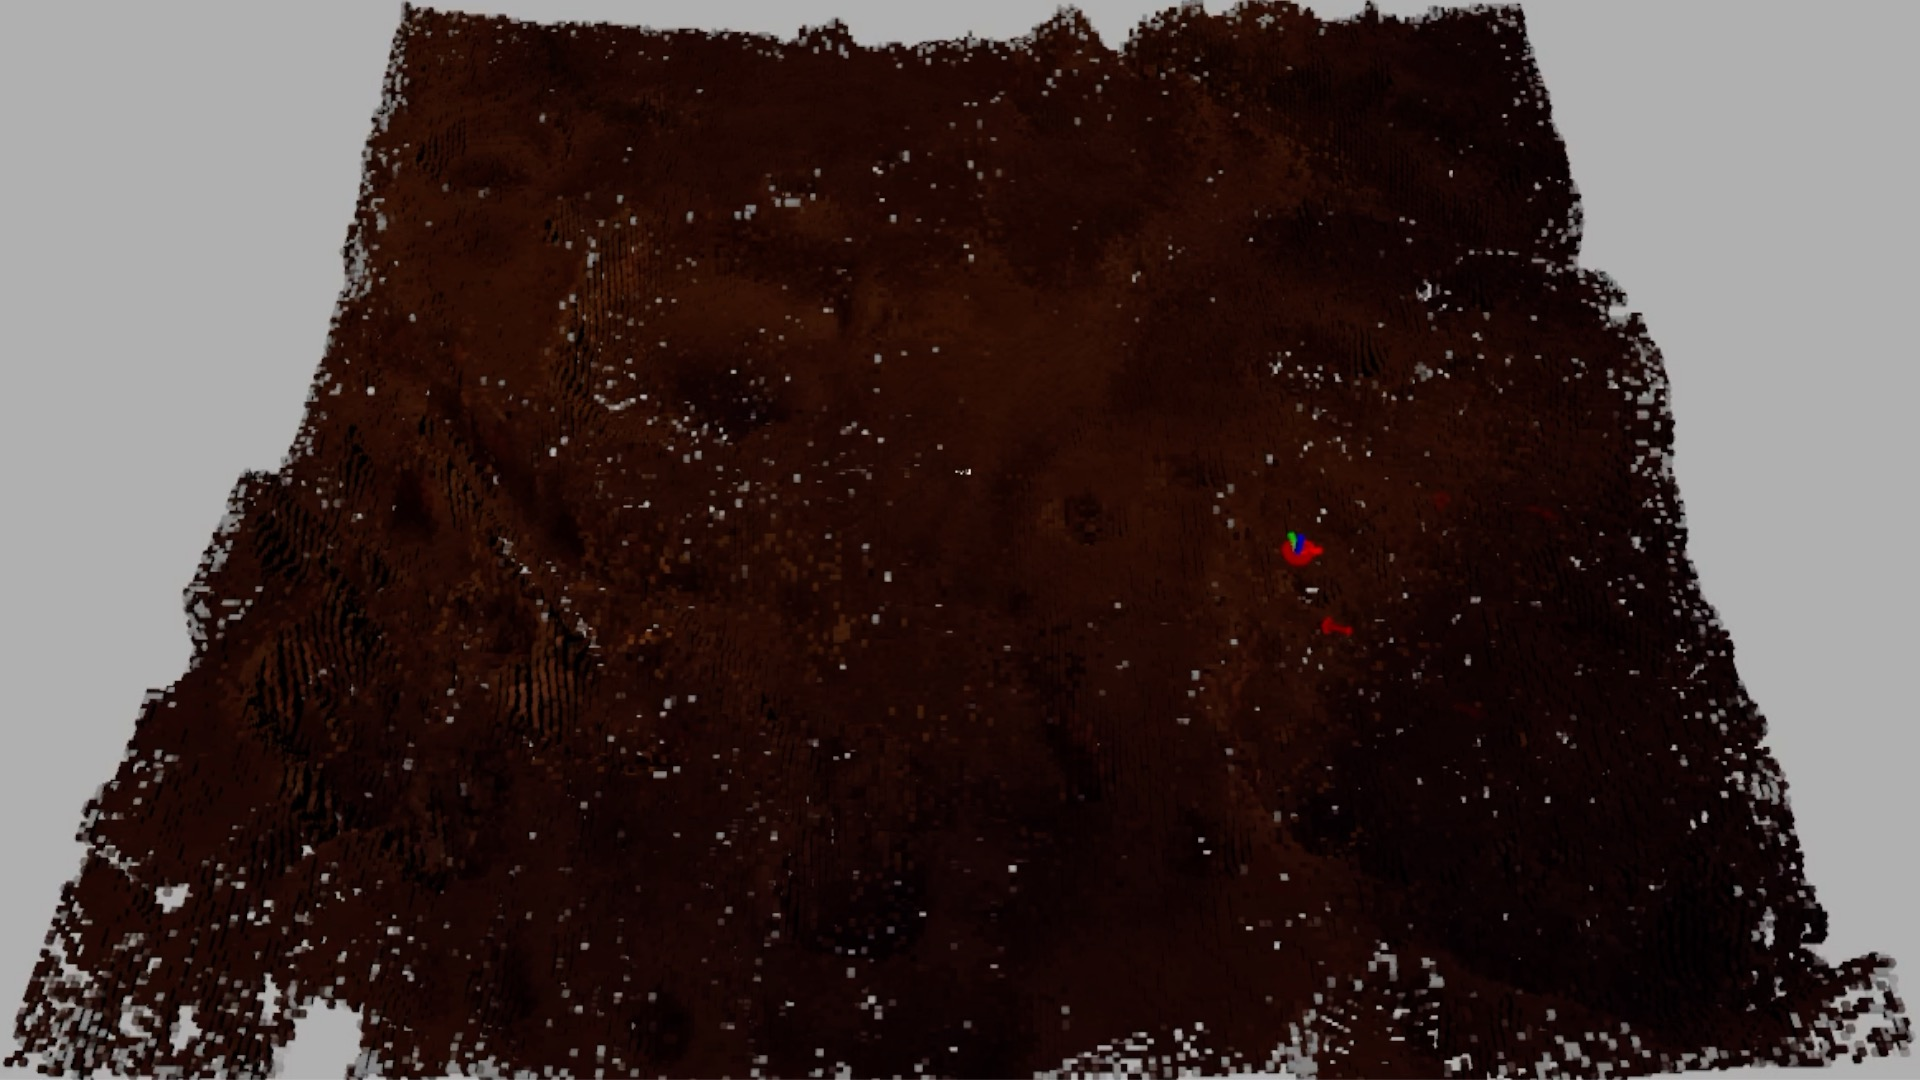
\includegraphics[height=0.5\textwidth]{MarsFullMap20min.jpg}
        		\caption{Case 1: $20$ min}
		\vspace*{0.025\textwidth}
    	\end{subfigure}
\caption{The robot (red disk with arrow indicating laser direction) moves toward candidate poses (red arrows, more opaque for greater reward) while generating a 3D probabilistic occupancy grid map (cubes: greater opacity for greater occupancy probability) of the surface of Mars.}
\label{fig:mars3Dogm}
=======
          	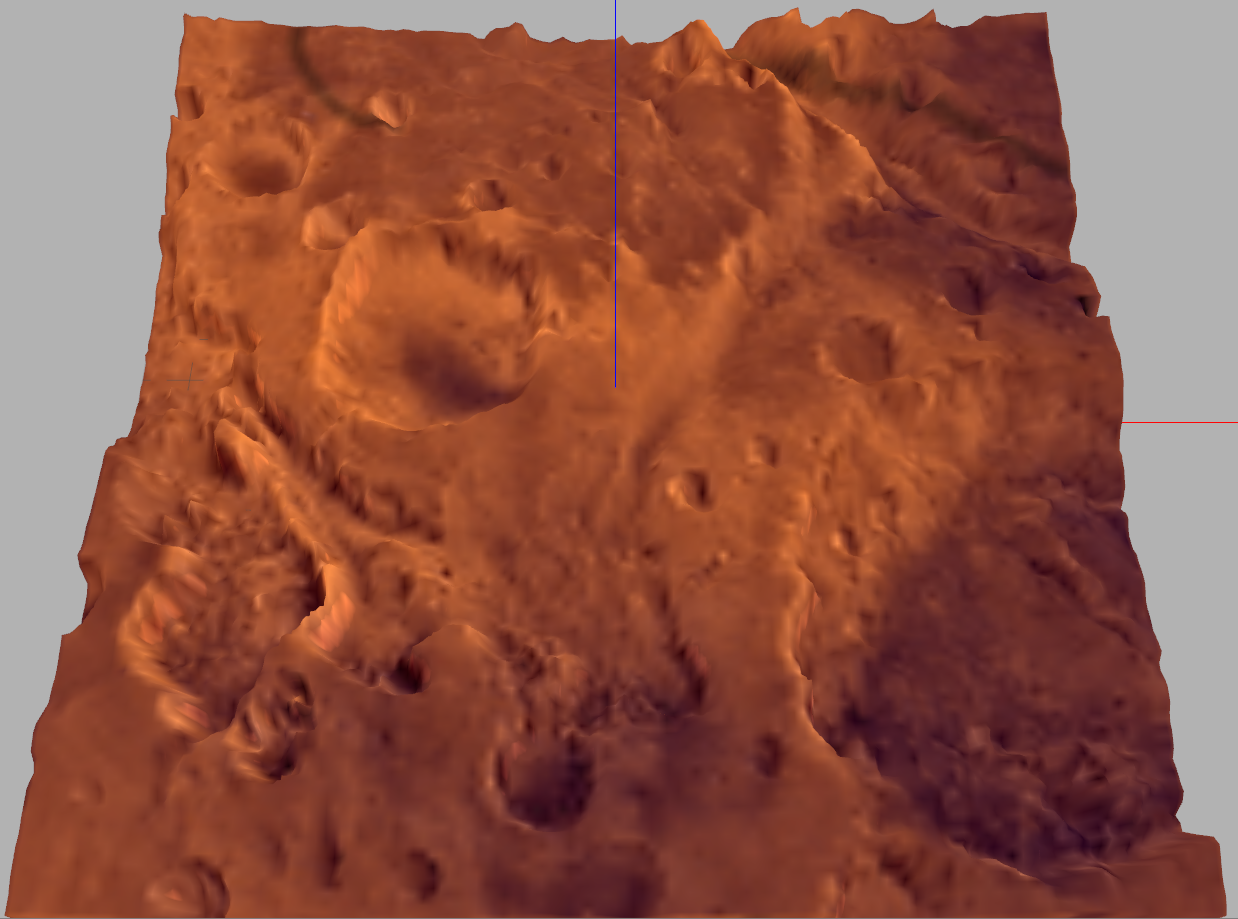
\includegraphics[height=0.9\textwidth]{mars_gazebo_full_lighting.png}}
        		\caption{Gazebo Environment}
    	\end{subfigure}
\caption{The height map (a) and color map (b) are combined in the Gazebo simulator (c) to model a Mars environment. The robot captures the simulated environment to generate an occupancy grid map.}
\label{fig:MarsGazebo}
\end{figure}

The map parameters are also important to the success of the exploration. The full map has dimensions $20$ m $\times$ $20$ m $\times$ $5$ m in the Mars-fixed frame, with cell edge length $\alpha=0.075$ m. The reduced map for collision-avoidance and motion planning has cells $k=3$ times the size ($0.225$ m), so $k^3=27$ cells are considered in \refeqn{Proj3DMapComb}. The bump functions use $f_\text{max}=1.0$, $f_\text{far}=0.1$, and $\beta=0.1$ to account for travel costs with \refeqn{BumpFunRecedingHorizon}. The receding horizon optimal time $d_\text{opt}$ is based on a fixed robot velocity of $0.25$ m/sec and the computation time varies from $1.8$ sec to $2.5$ sec.

The simulation was run twice. Case 1 was as described in this paper. Case 2 was identical to Case 1, except the reduced map $ m_\text{reduced}$ is used when computing \refeqn{Iscan}. Case 2 is largely inspired by the promising results of~\cite{KauTakAiLee18}, where a projected map based on the same criteria as \refeqn{Proj3DMapComb} proved effective for level flight. The resulting occupancy grid maps for Cases 1 and 2 are shown in Figs. \ref{fig:mars3DogmCase1} and \ref{fig:mars3DogmCase2}, respectively. A video of Case 1 can be found at \href{https://youtu.be/FrBcL2UMW9w}{https://youtu.be/FrBcL2UMW9w} and close-up pictures from Case 2 are shown in Fig. \ref{fig:marsZoomedIn}. The complete map entropy is illustrated in Fig. \ref{fig:mars3Dentropy}.

%\begin{figure}[!t]
%	\centering
%	\begin{subfigure}[t]{0.4\columnwidth}
%           	\centering
%          	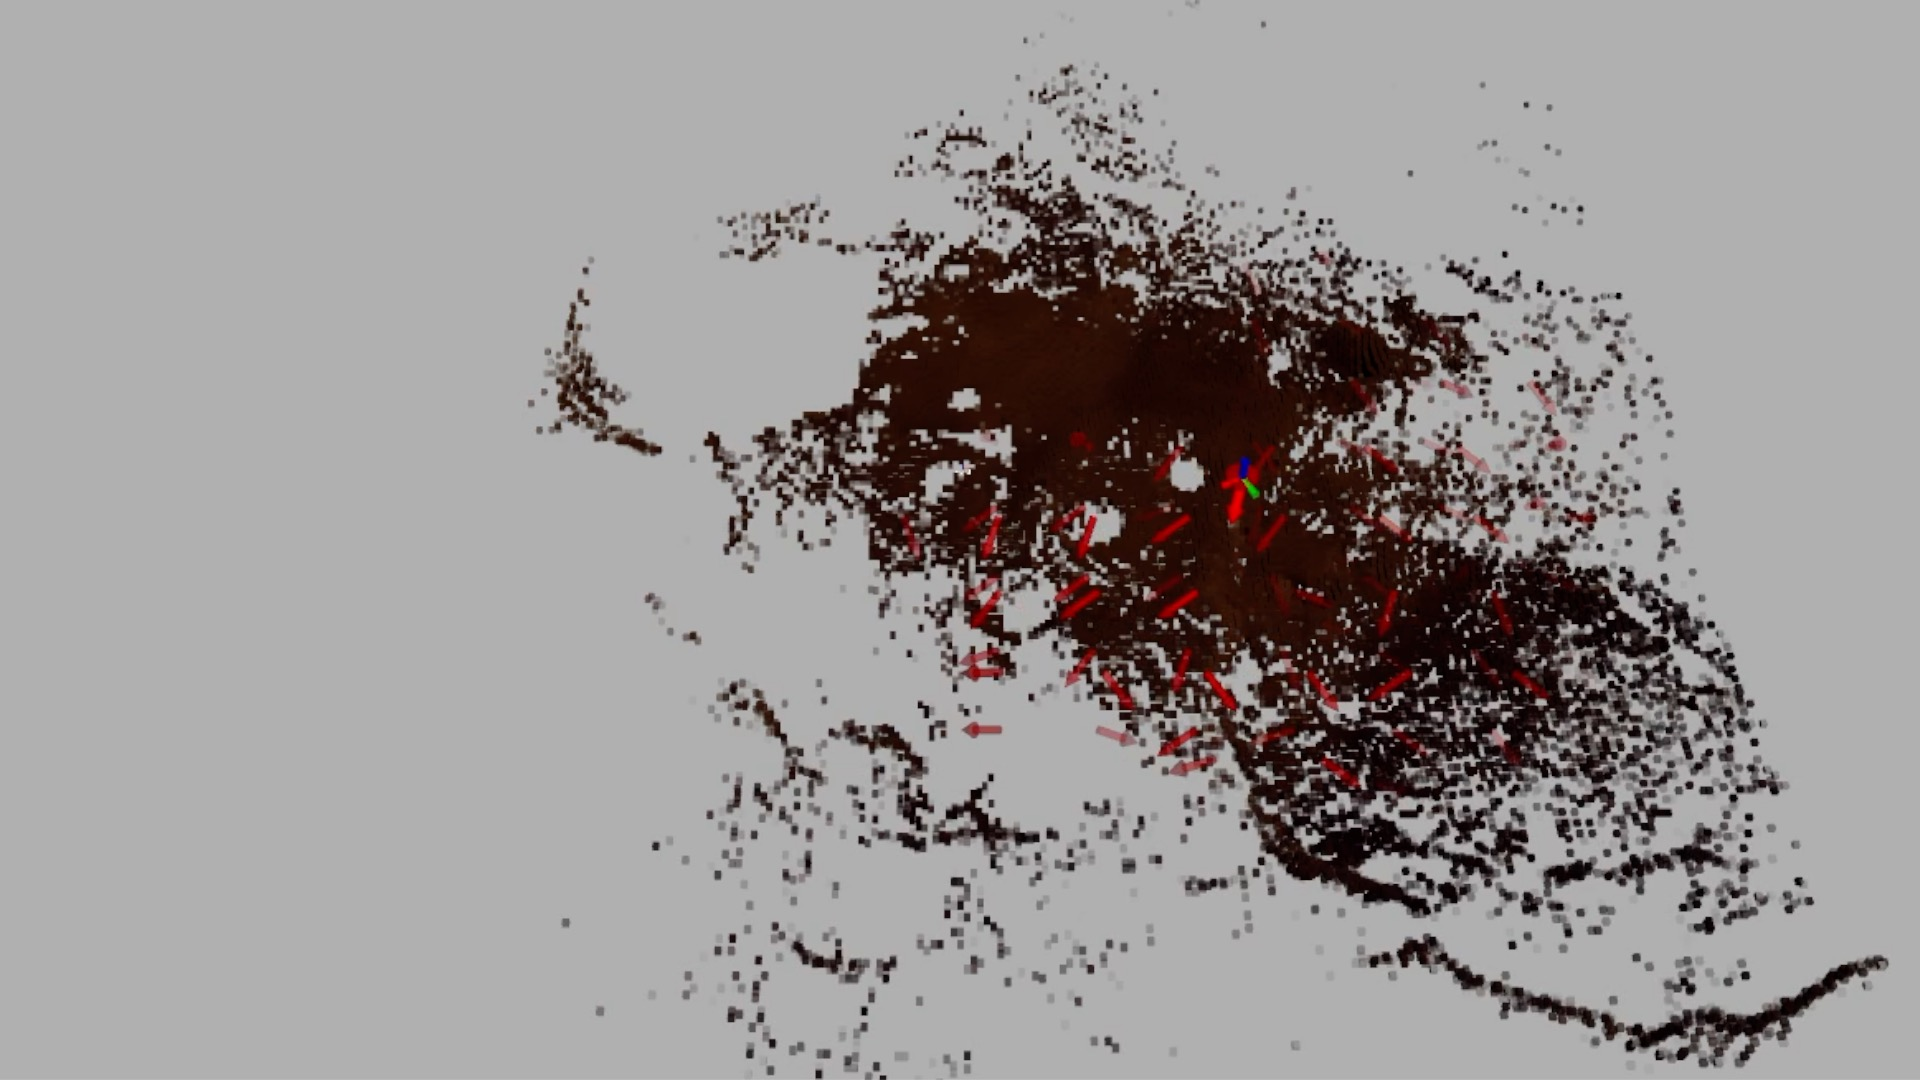
\includegraphics[height=0.5\textwidth]{MarsFullMap1min.jpg}
%        		\caption{Case 1: $1$ min}
%		\vspace*{0.025\textwidth}
%    	\end{subfigure}
%    	\begin{subfigure}[t]{0.4\columnwidth}
%           	\centering
%          	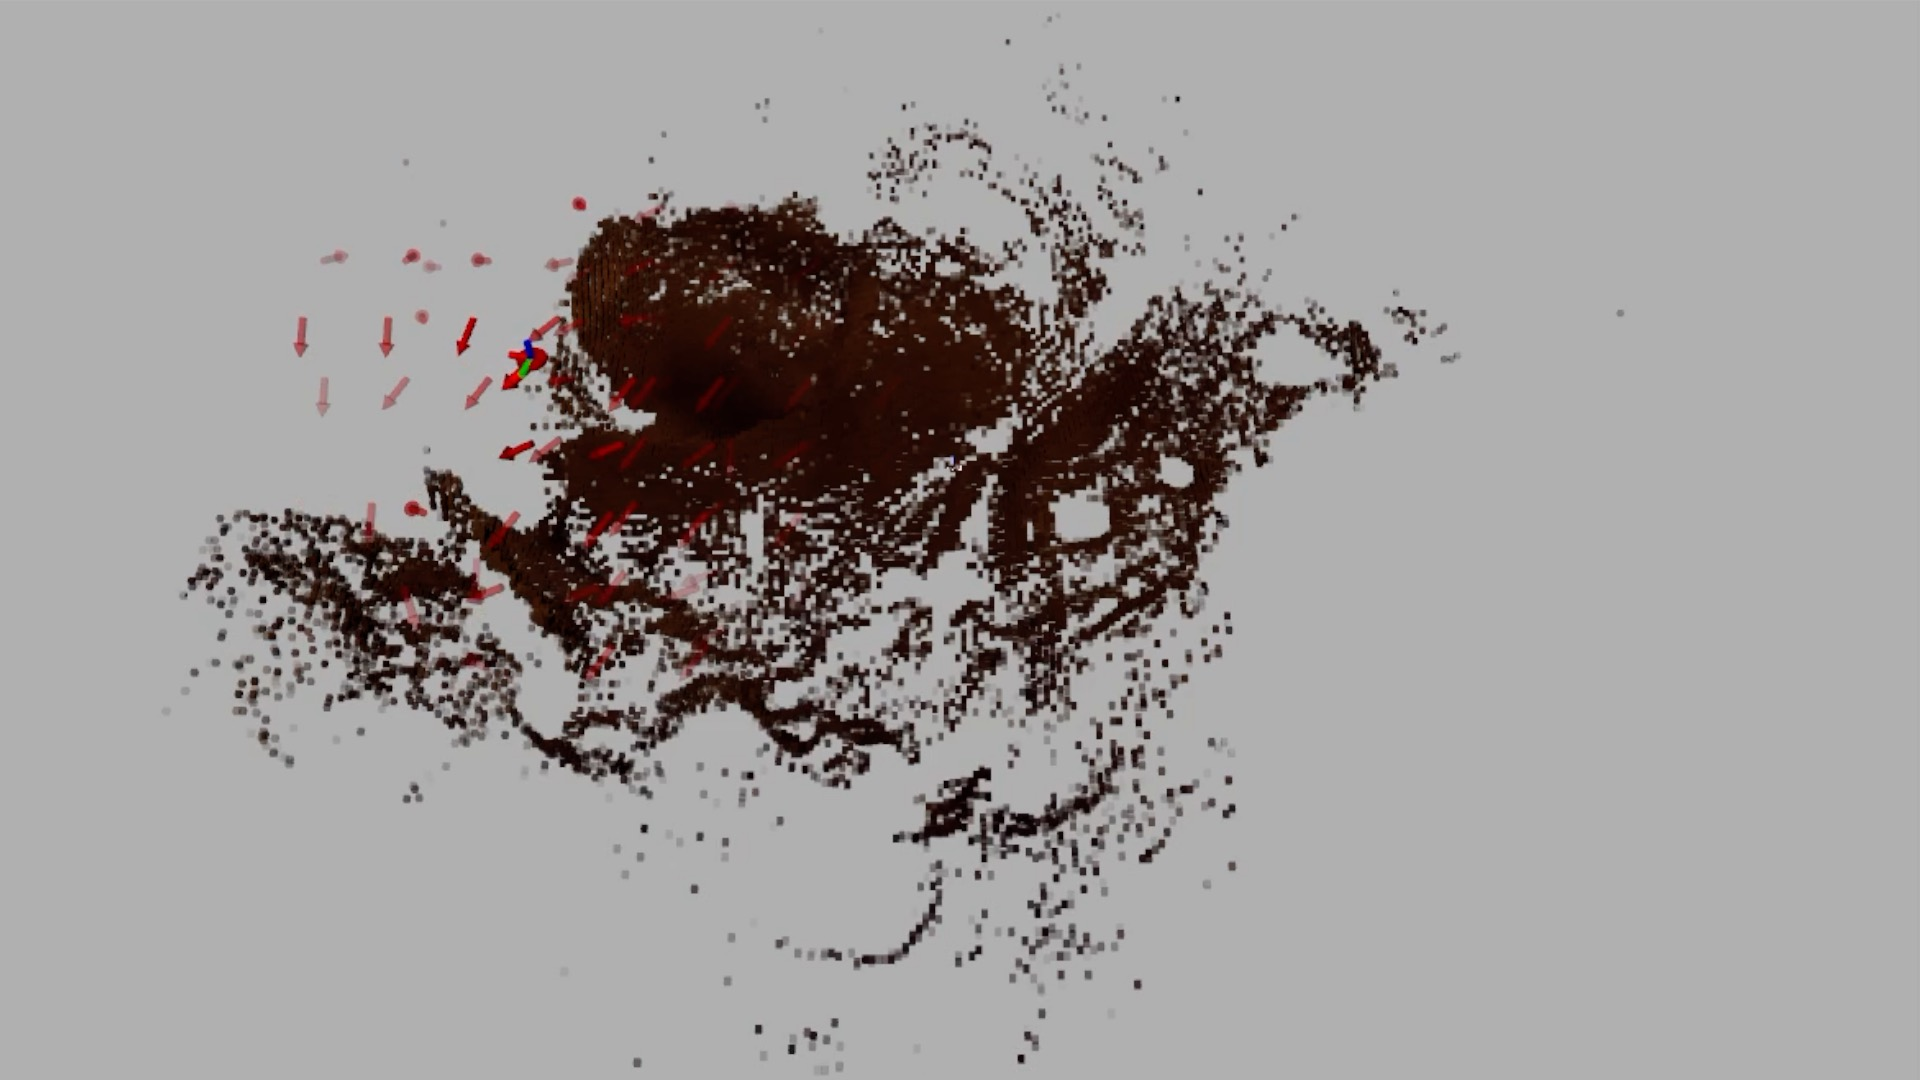
\includegraphics[height=0.5\textwidth]{MarsRdcdMap1min.jpg}
%        		\caption{Case 2: $1$ min}
%		\vspace*{0.025\textwidth}
%    	\end{subfigure}
%	\centering
%	\begin{subfigure}[t]{0.4\columnwidth}
%           	\centering
%          	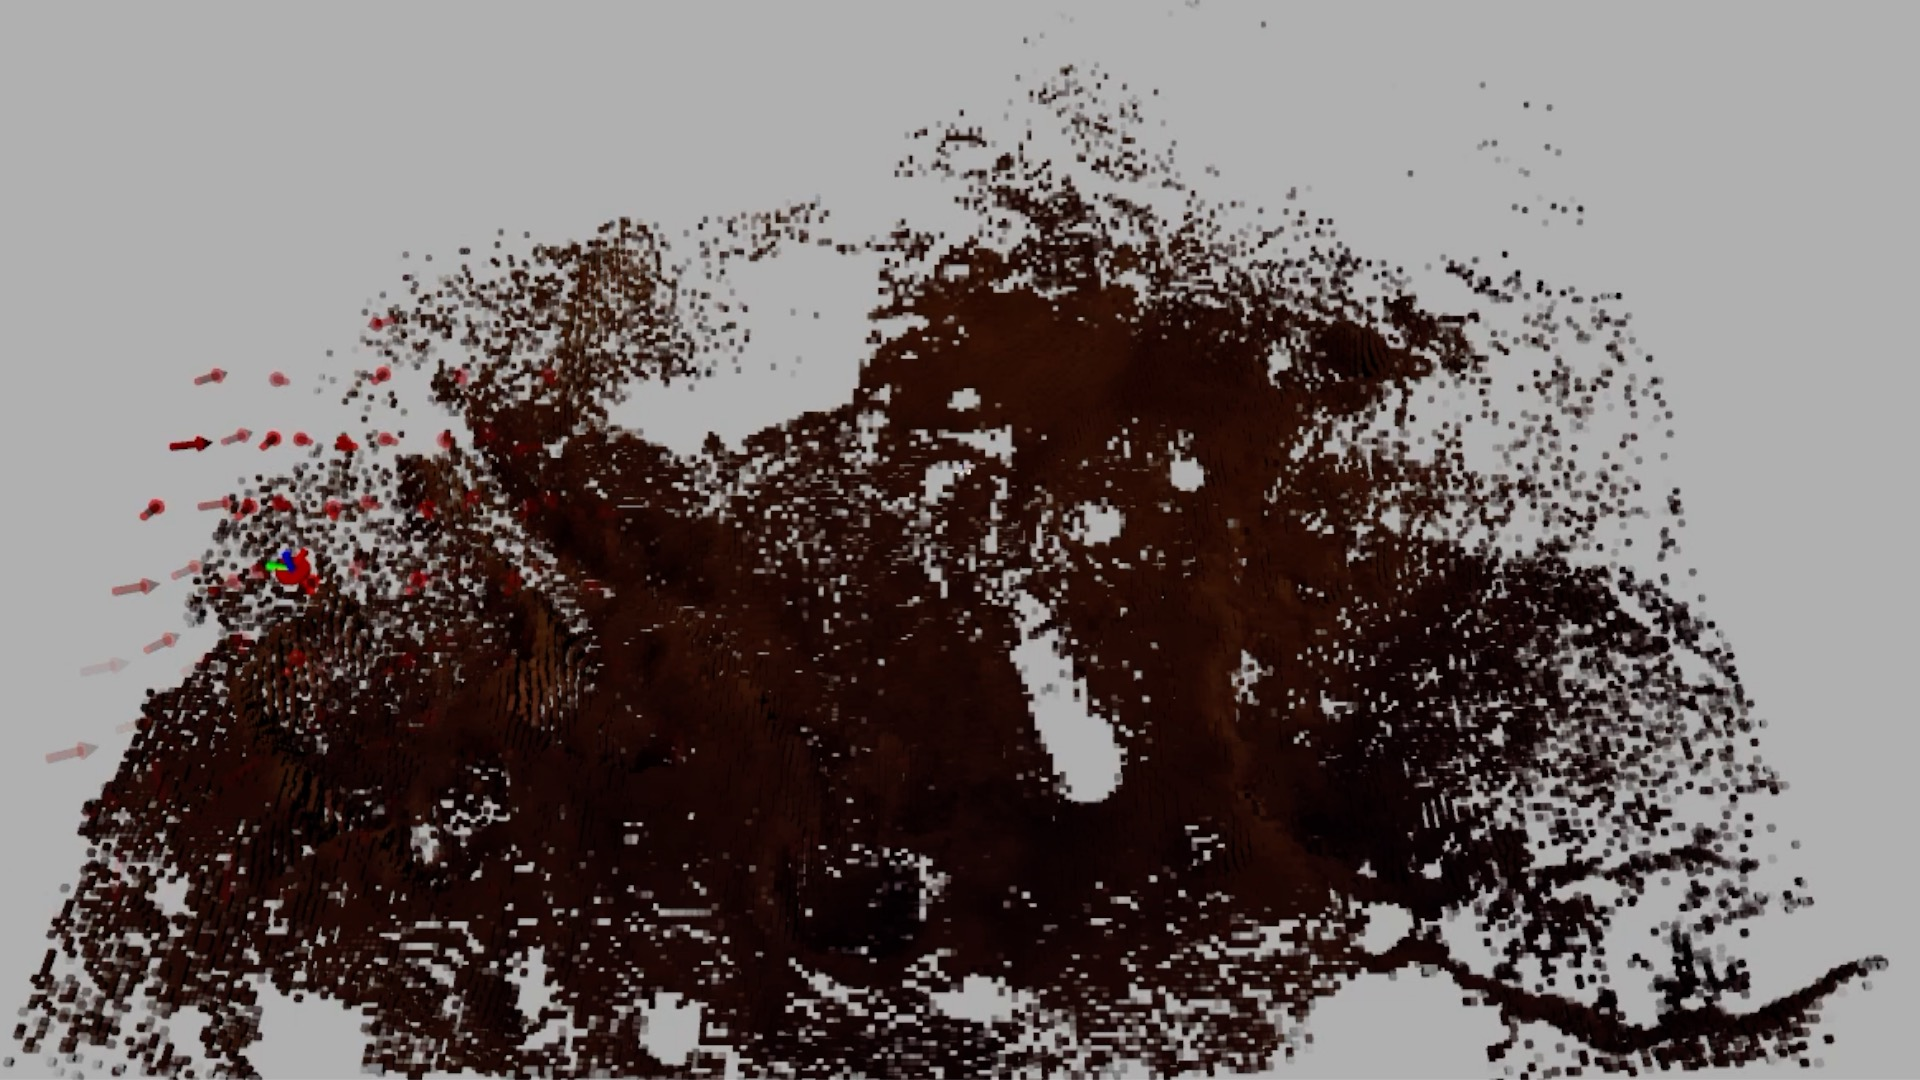
\includegraphics[height=0.5\textwidth]{MarsFullMap2min.jpg}
%        		\caption{Case 1: $2$ min}
%		\vspace*{0.025\textwidth}
%    	\end{subfigure}
%    	\begin{subfigure}[t]{0.4\columnwidth}
%           	\centering
%          	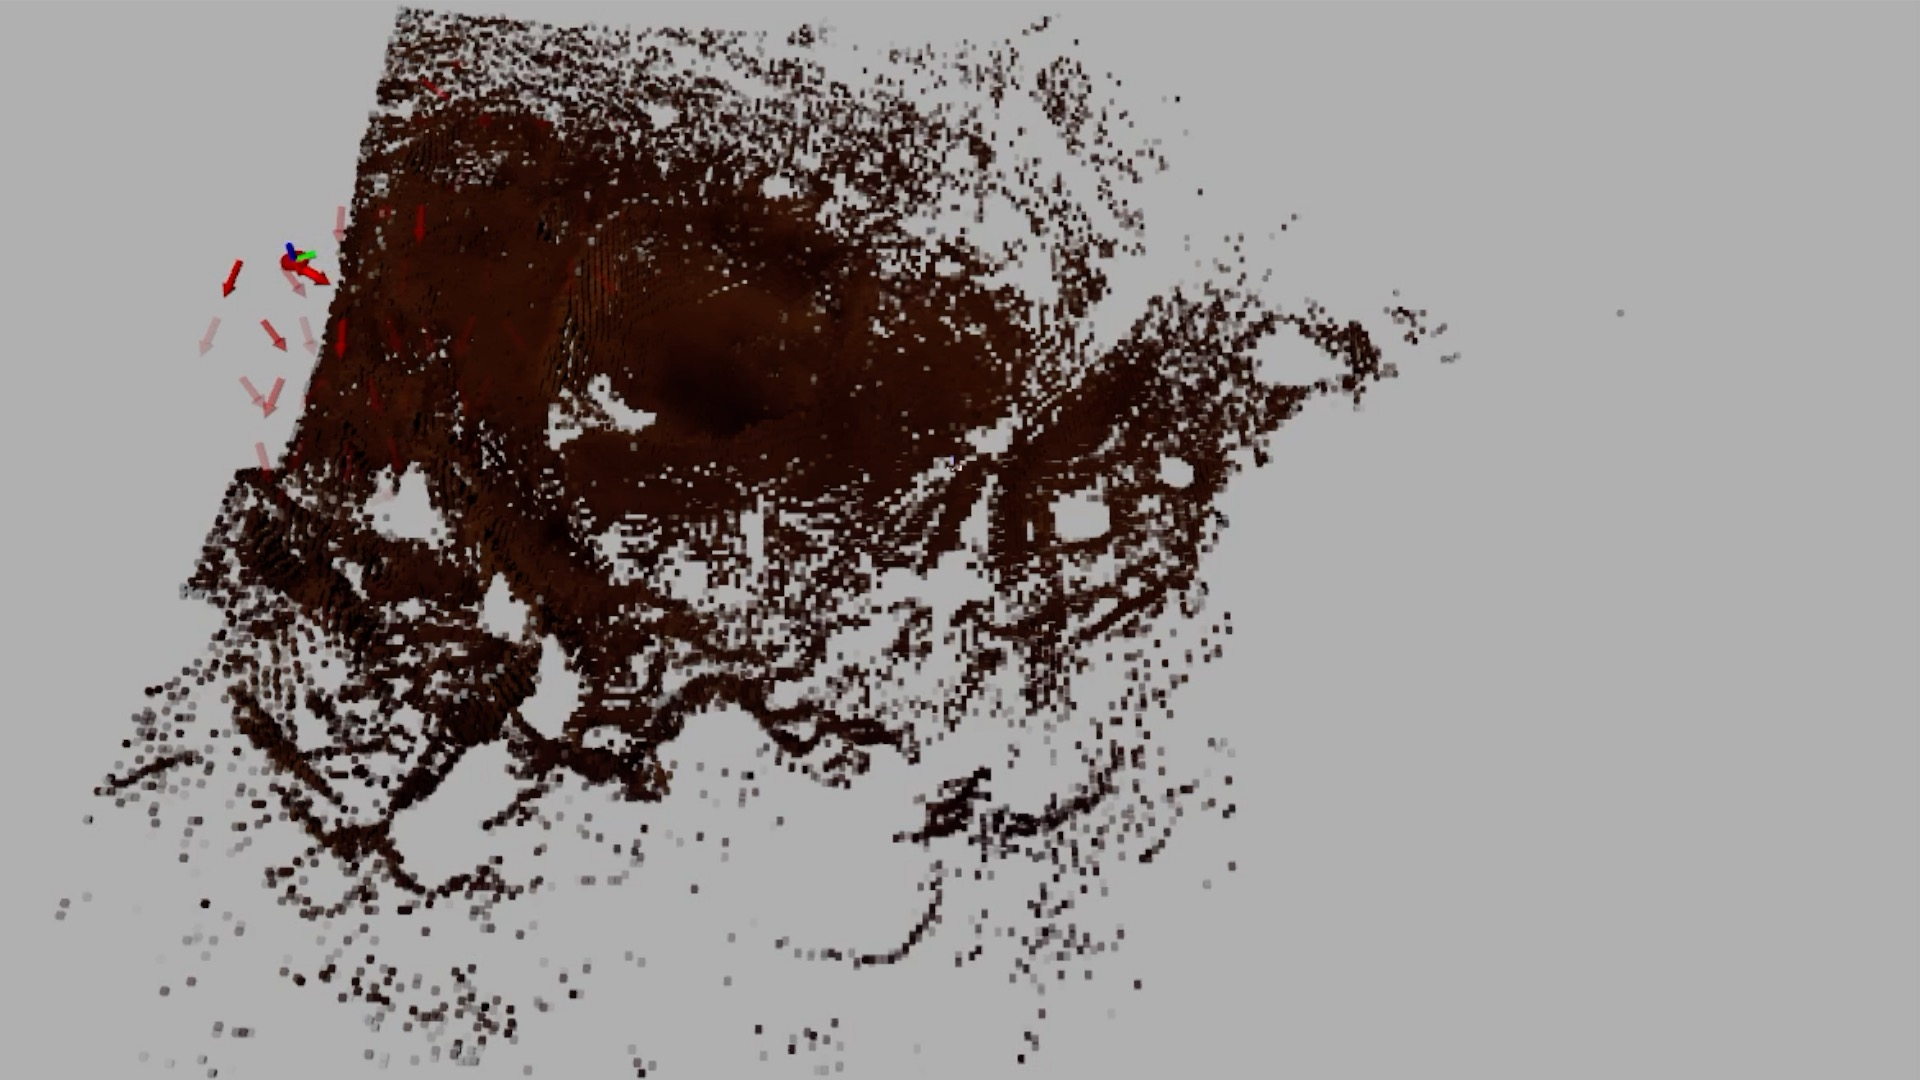
\includegraphics[height=0.5\textwidth]{MarsRdcdMap2min.jpg}
%        		\caption{Case 2: $2$ min}
%		\vspace*{0.025\textwidth}
%    	\end{subfigure}
%	\centering
%	\begin{subfigure}[t]{0.4\columnwidth}
%           	\centering
%          	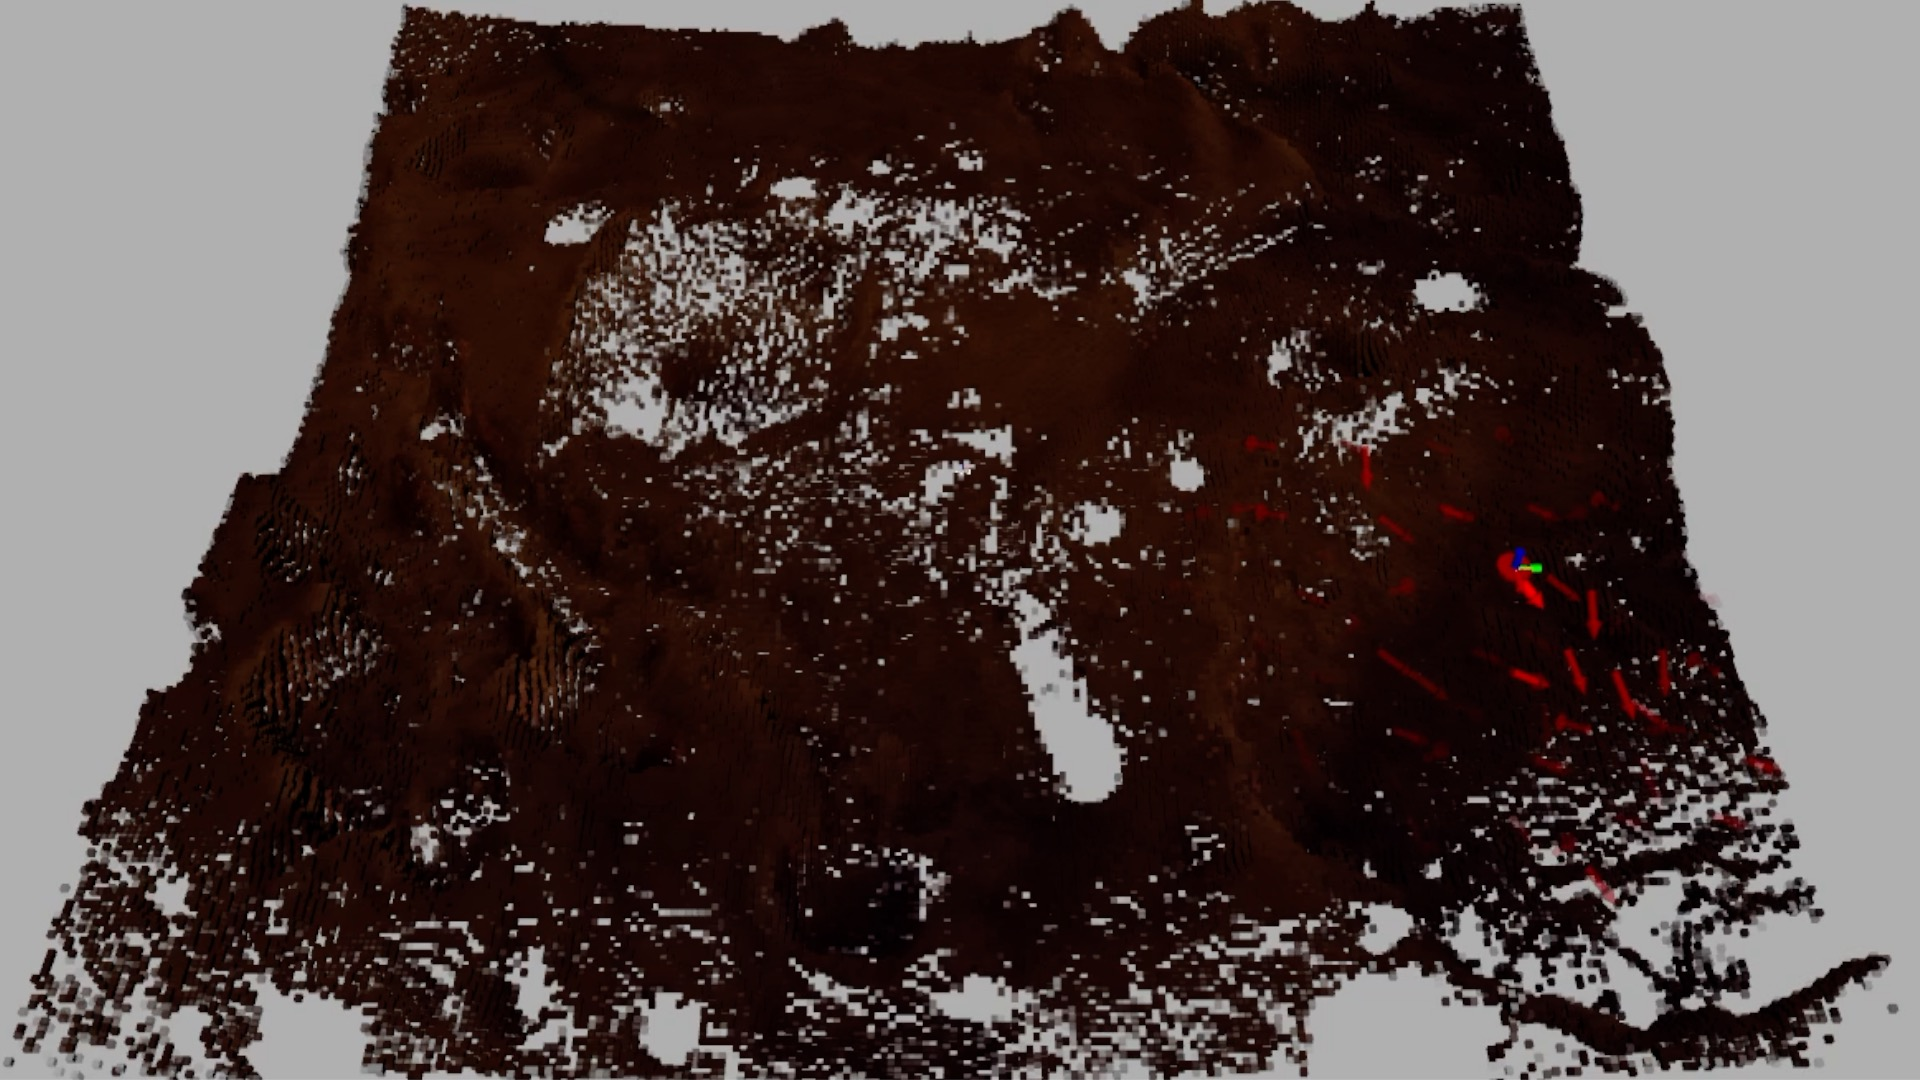
\includegraphics[height=0.5\textwidth]{MarsFullMap5min.jpg}
%        		\caption{Case 1: $5$ min}
%		\vspace*{0.025\textwidth}
%    	\end{subfigure}
%    	\begin{subfigure}[t]{0.4\columnwidth}
%           	\centering
%          	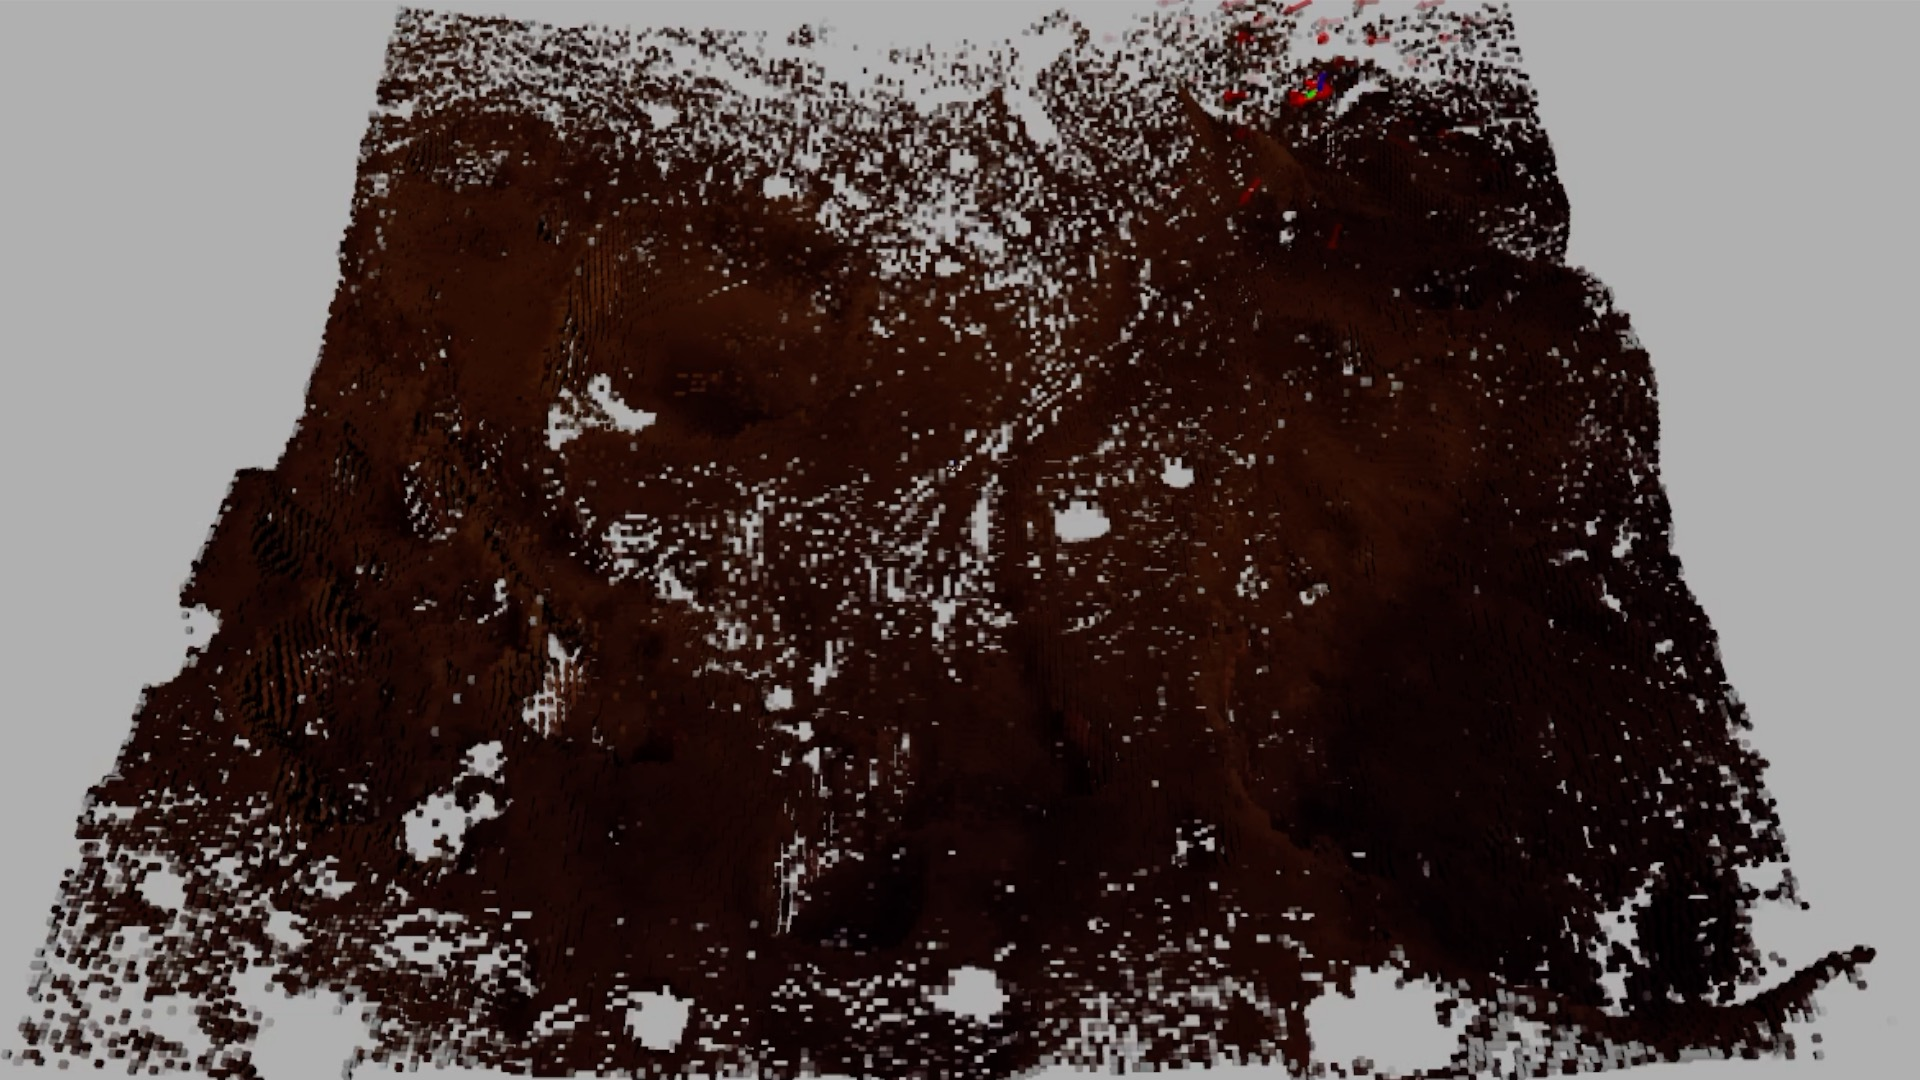
\includegraphics[height=0.5\textwidth]{MarsRdcdMap5min.jpg}
%        		\caption{Case 2: $5$ min}
%		\vspace*{0.025\textwidth}
%    	\end{subfigure}
%	\centering
%	\begin{subfigure}[t]{0.4\columnwidth}
%           	\centering
%          	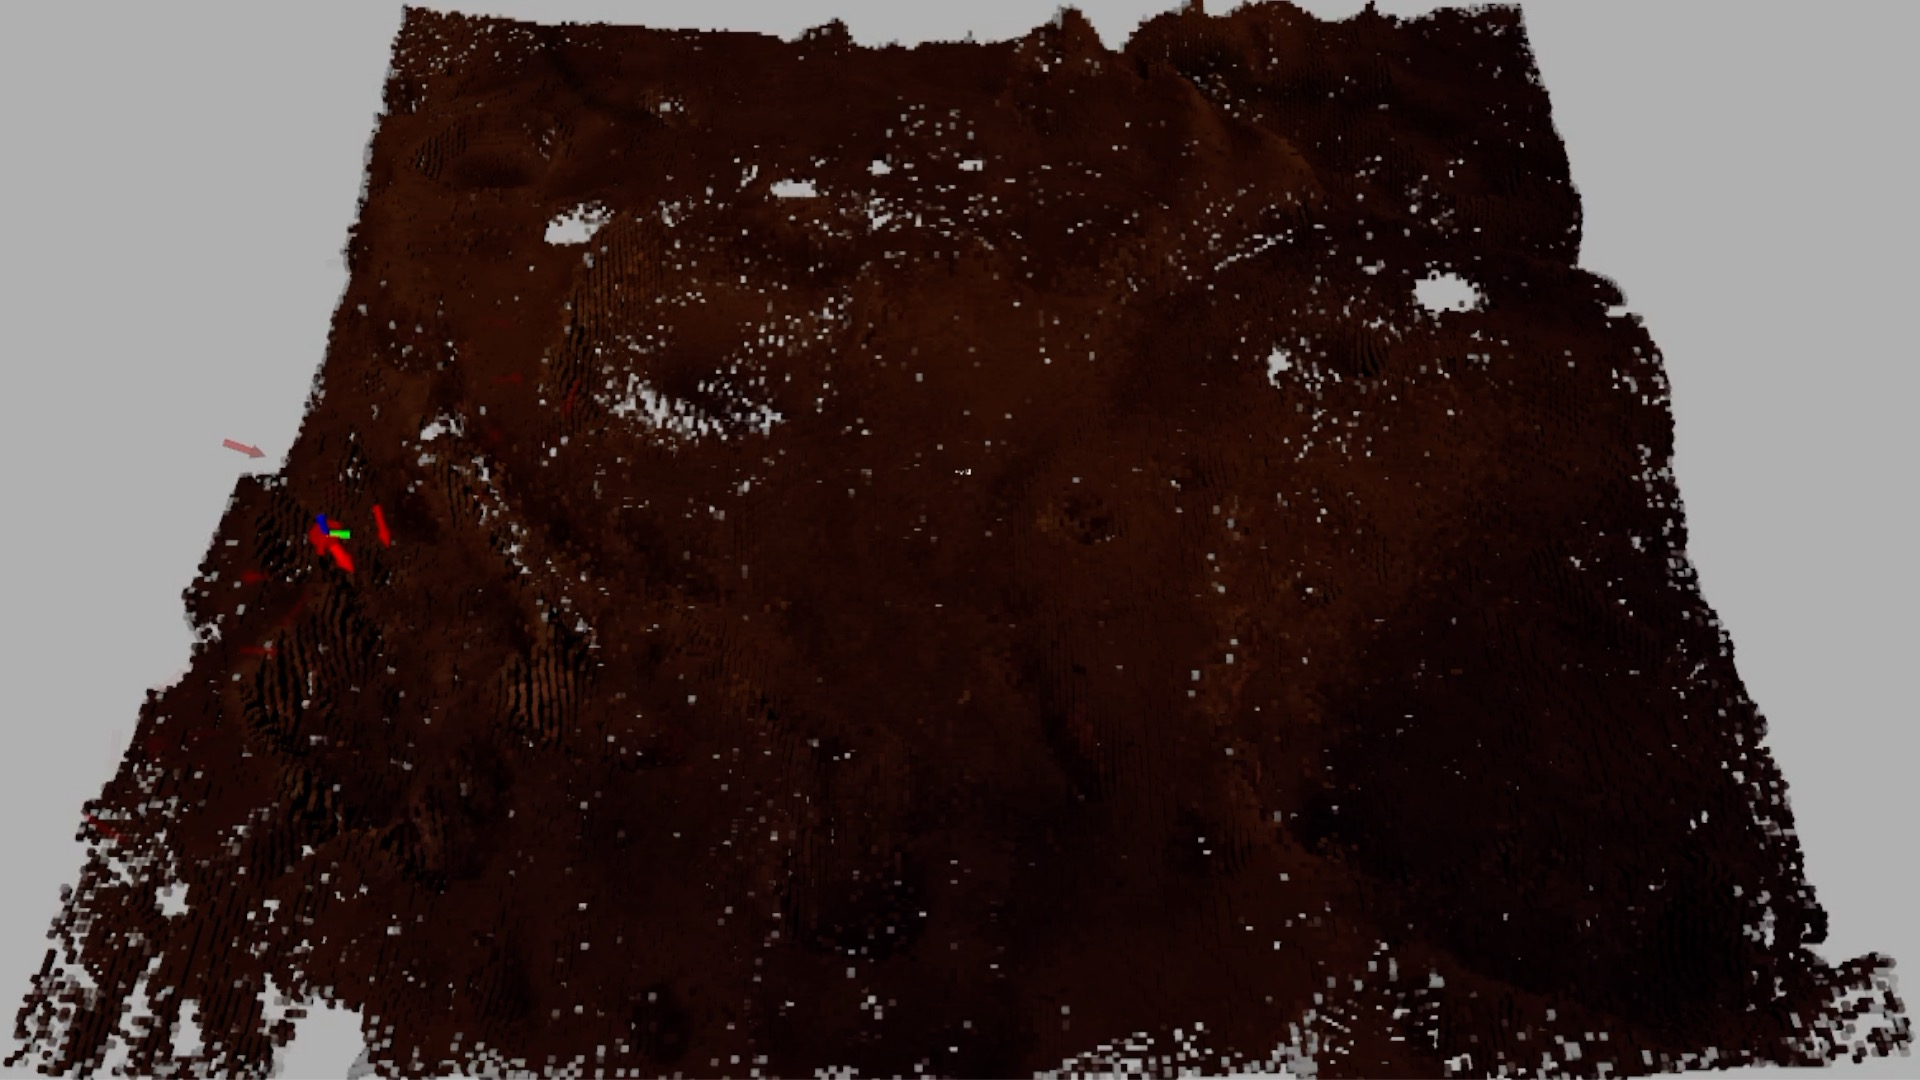
\includegraphics[height=0.5\textwidth]{MarsFullMap10min.jpg}
%        		\caption{Case 1: $10$ min}
%		\vspace*{0.025\textwidth}
%    	\end{subfigure}
%    	\begin{subfigure}[t]{0.4\columnwidth}
%           	\centering
%          	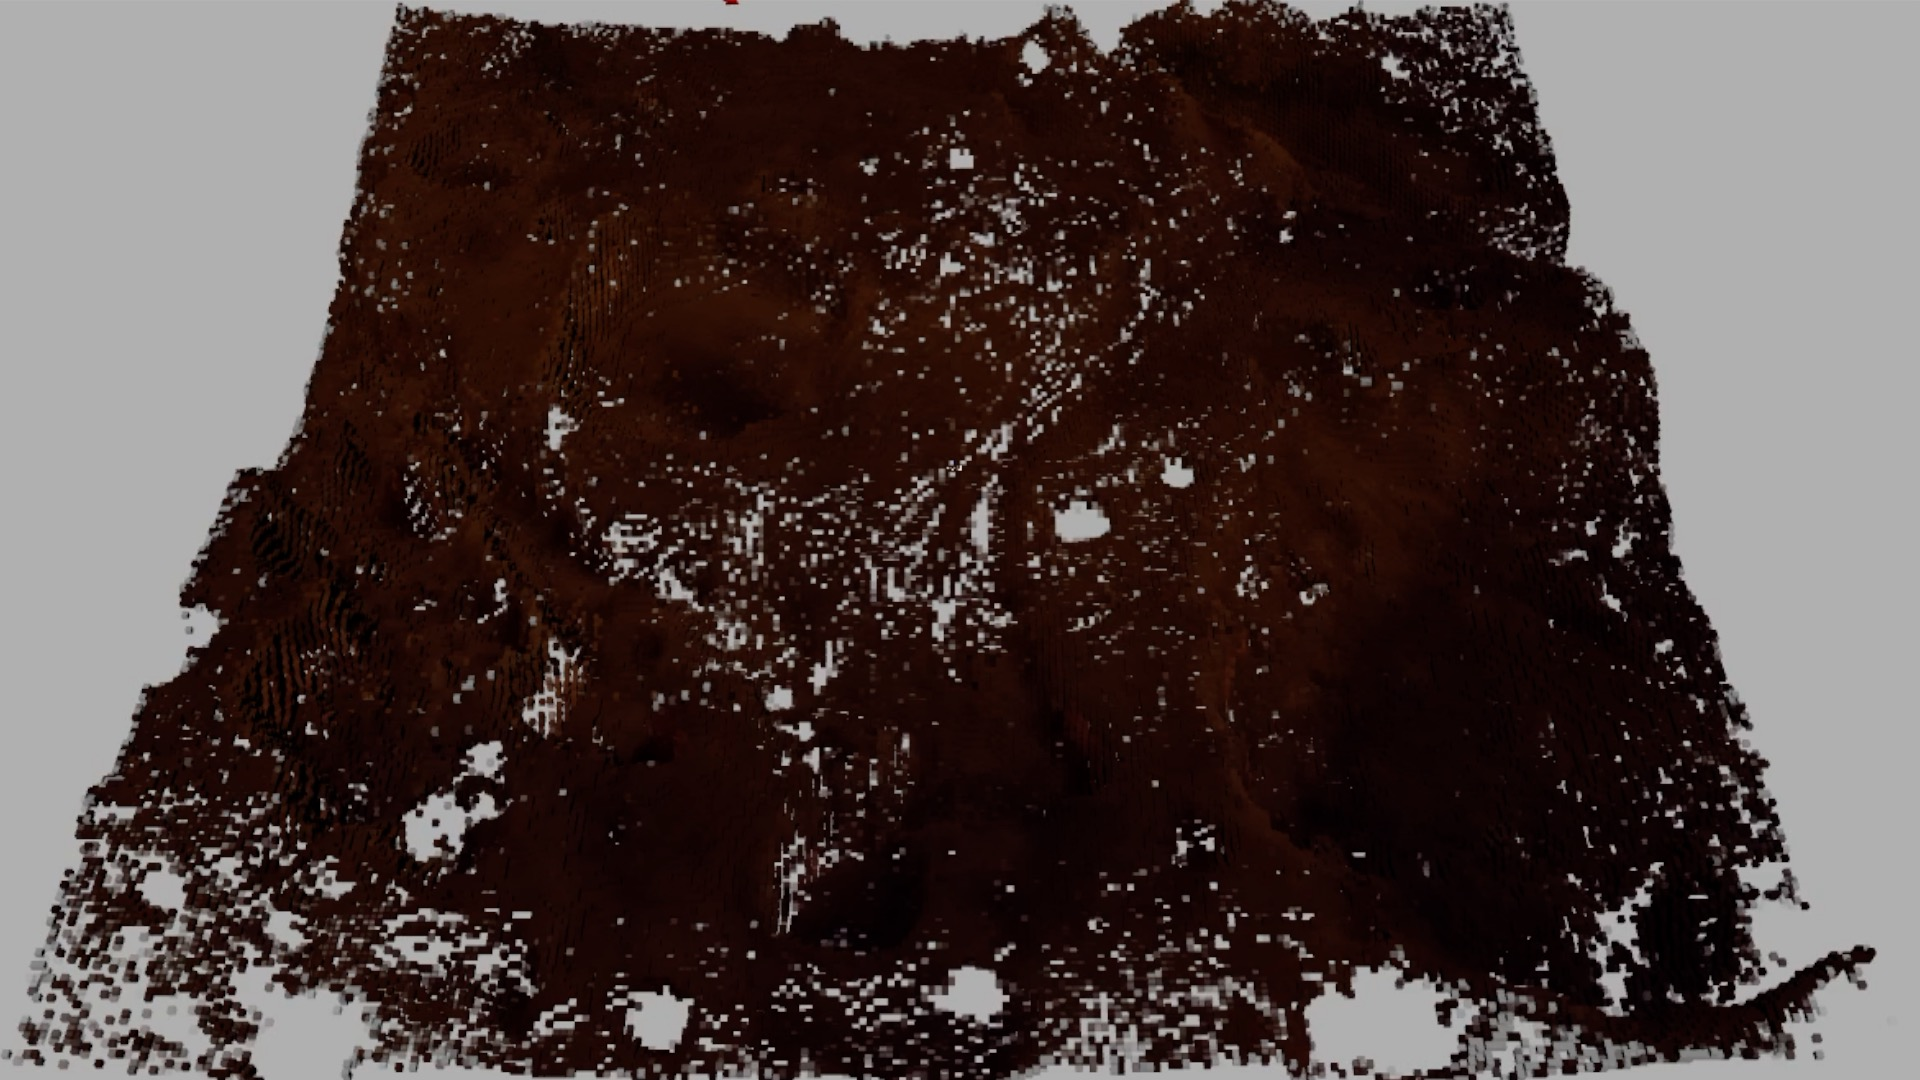
\includegraphics[height=0.5\textwidth]{MarsRdcdMap10min.jpg}
%        		\caption{Case 2: $10$ min}
%		\vspace*{0.025\textwidth}
%    	\end{subfigure}
%	\centering
%	\begin{subfigure}[t]{0.4\columnwidth}
%           	\centering
%          	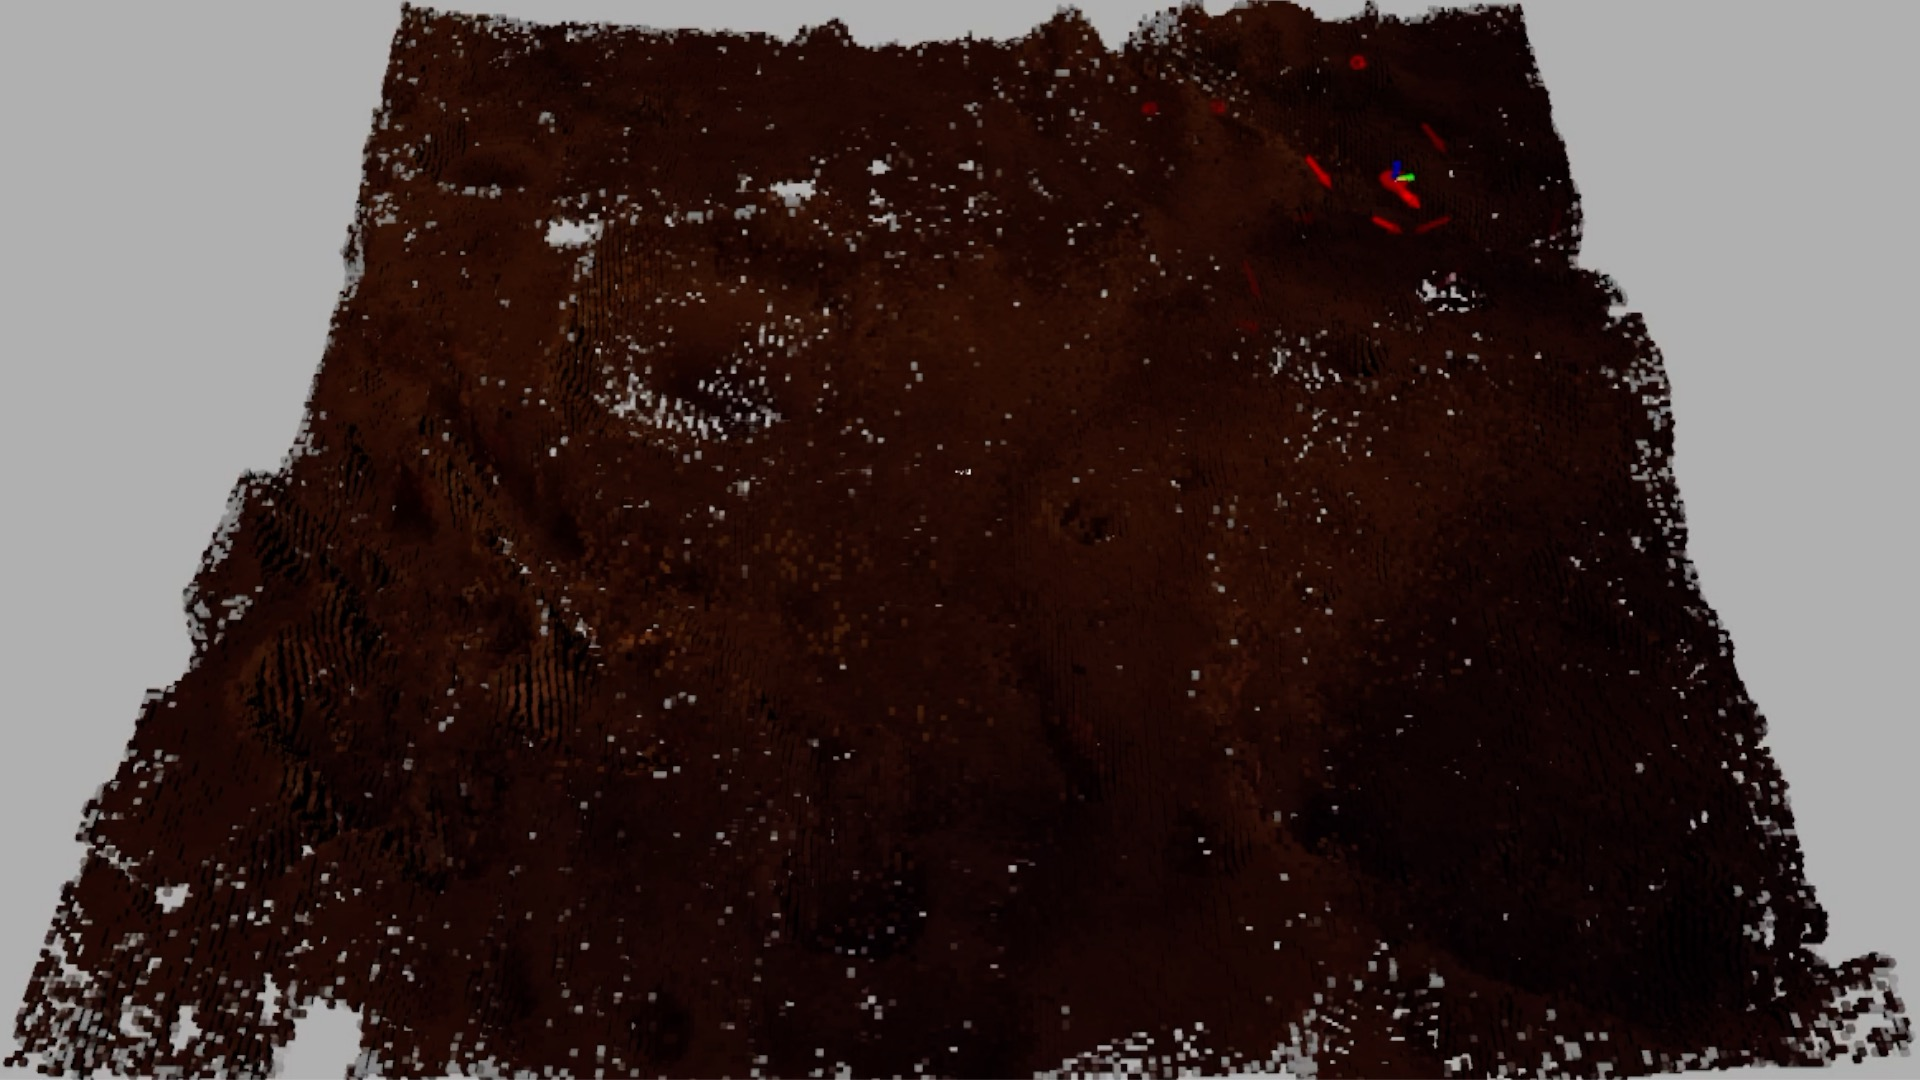
\includegraphics[height=0.5\textwidth]{MarsFullMap15min.jpg}
%        		\caption{Case 1: $15$ min}
%		\vspace*{0.025\textwidth}
%    	\end{subfigure}
%    	\begin{subfigure}[t]{0.4\columnwidth}
%           	\centering
%          	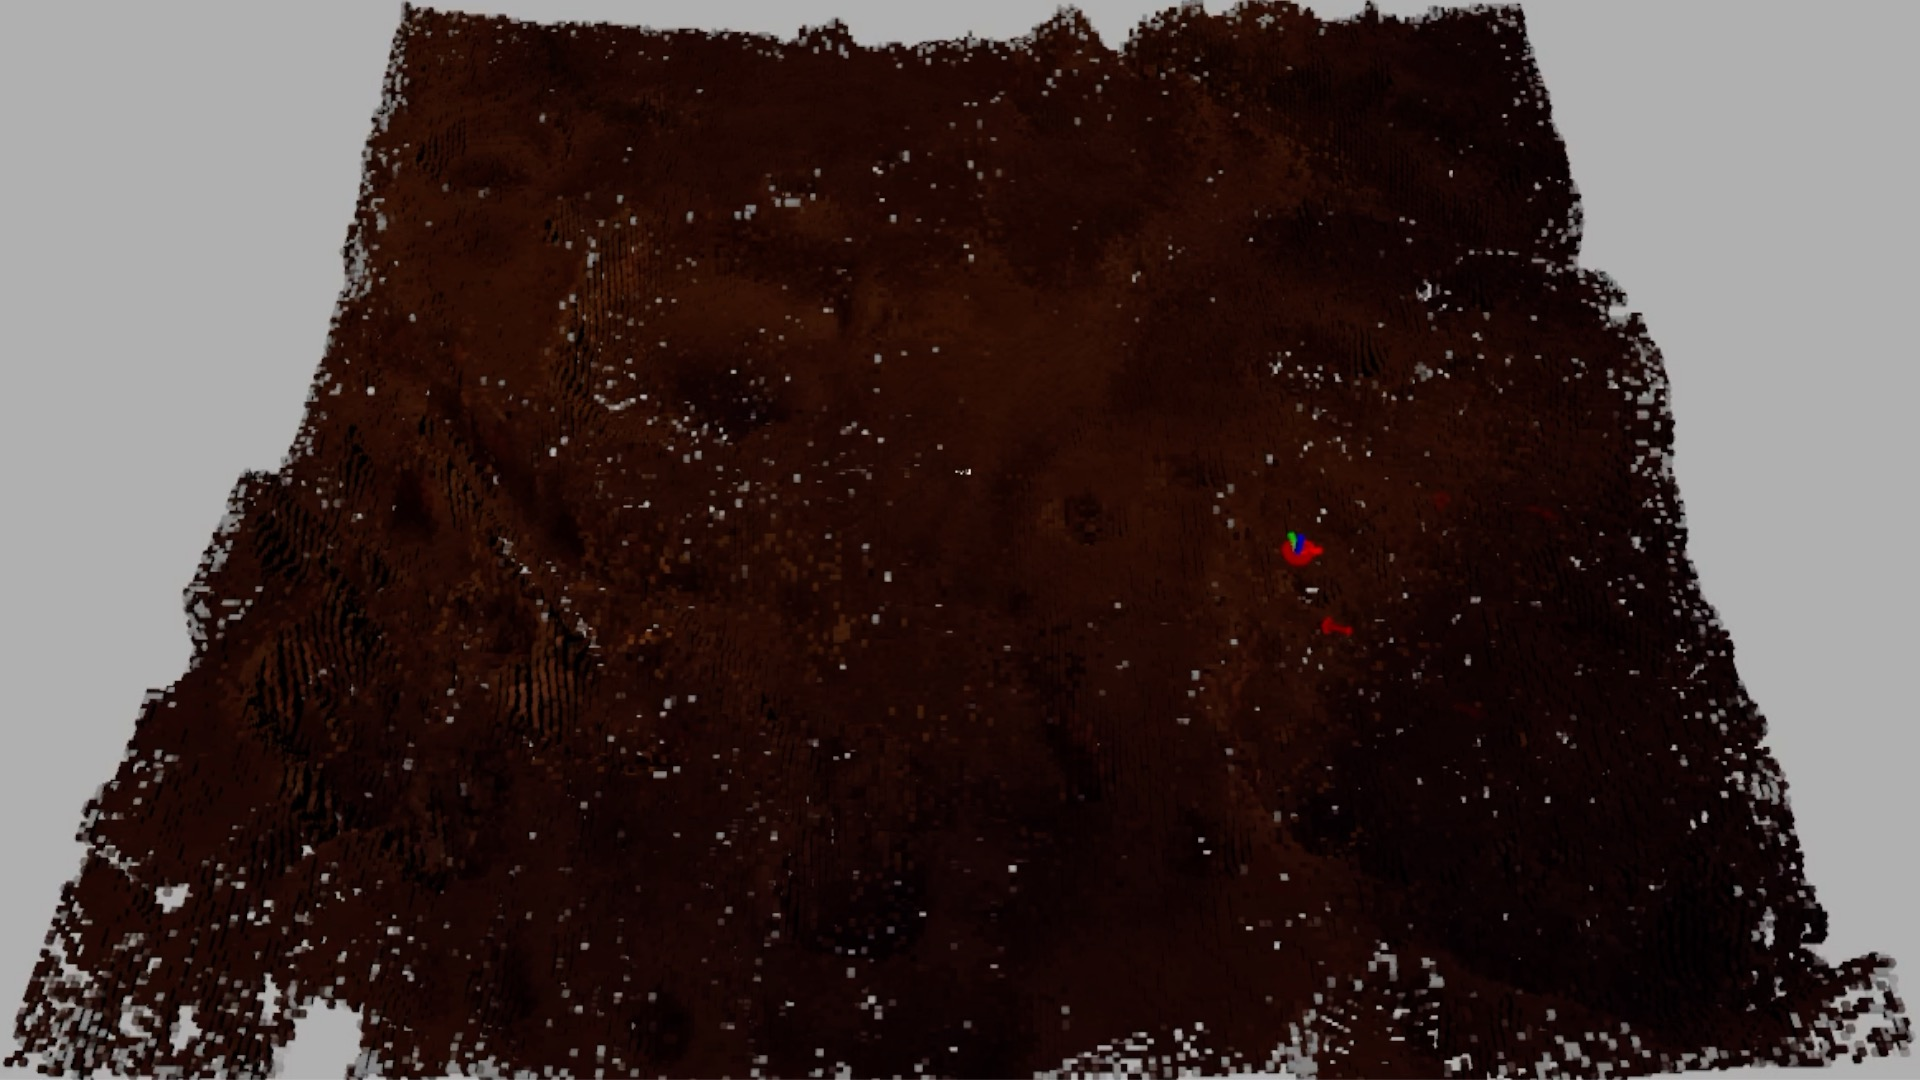
\includegraphics[height=0.5\textwidth]{MarsFullMap20min.jpg}
%        		\caption{Case 1: $20$ min}
%		\vspace*{0.025\textwidth}
%    	\end{subfigure}
%\caption{The robot (red disk with arrow indicating laser direction) moves toward candidate poses (red arrows, more opaque for greater reward) while generating a 3D probabilistic occupancy grid map (cubes: greater opacity for greater occupancy probability) of the surface of Mars.}
%\label{fig:mars3Dogm}
%\end{figure}


\begin{figure}[!t]
	\centering
	\begin{subfigure}[t]{0.49\columnwidth}
           	\centering
          	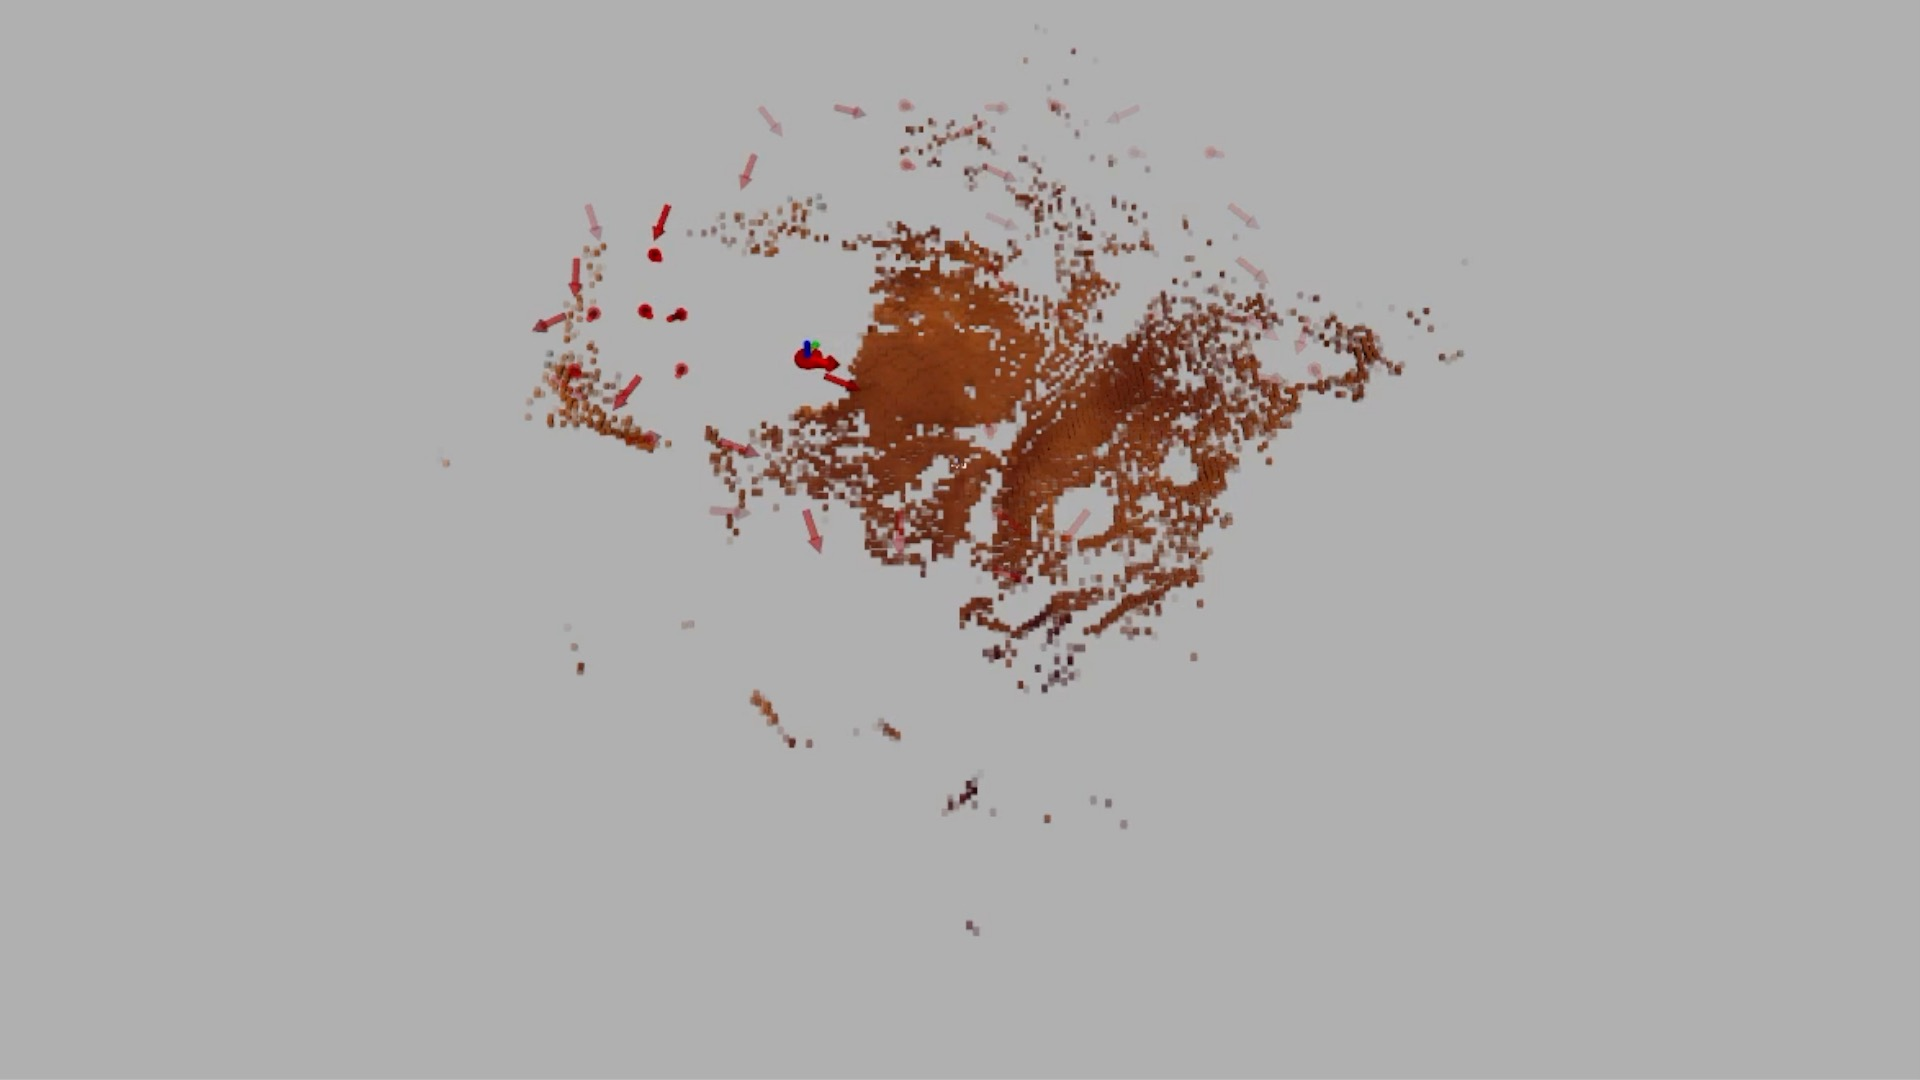
\includegraphics[height=0.5\textwidth]{FullMarsMap30sec.jpg}
        		\caption{$30$ sec}
		\vspace*{0.025\textwidth}
    	\end{subfigure}
    	\begin{subfigure}[t]{0.49\columnwidth}
           	\centering
          	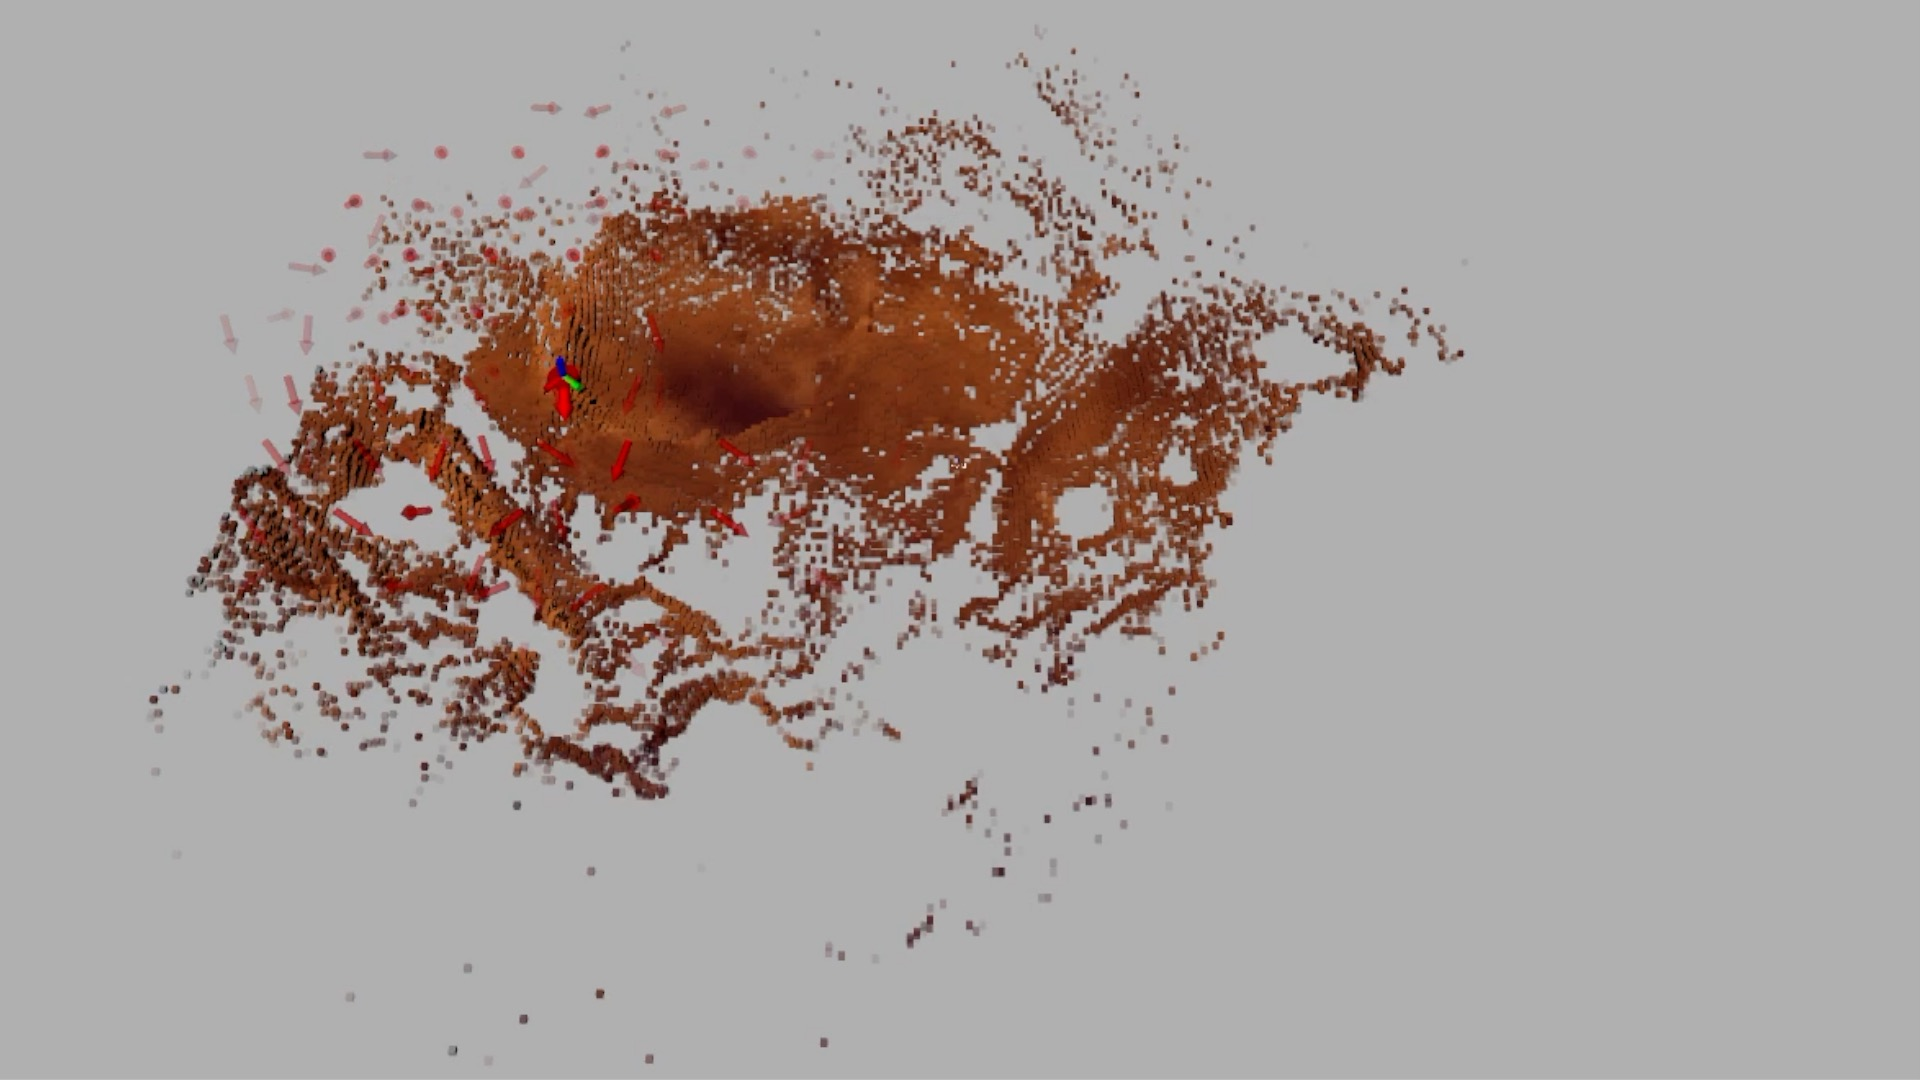
\includegraphics[height=0.5\textwidth]{FullMarsMap1min.jpg}
        		\caption{$1$ min}
		\vspace*{0.025\textwidth}
    	\end{subfigure}
	\centering
	\begin{subfigure}[t]{0.49\columnwidth}
           	\centering
          	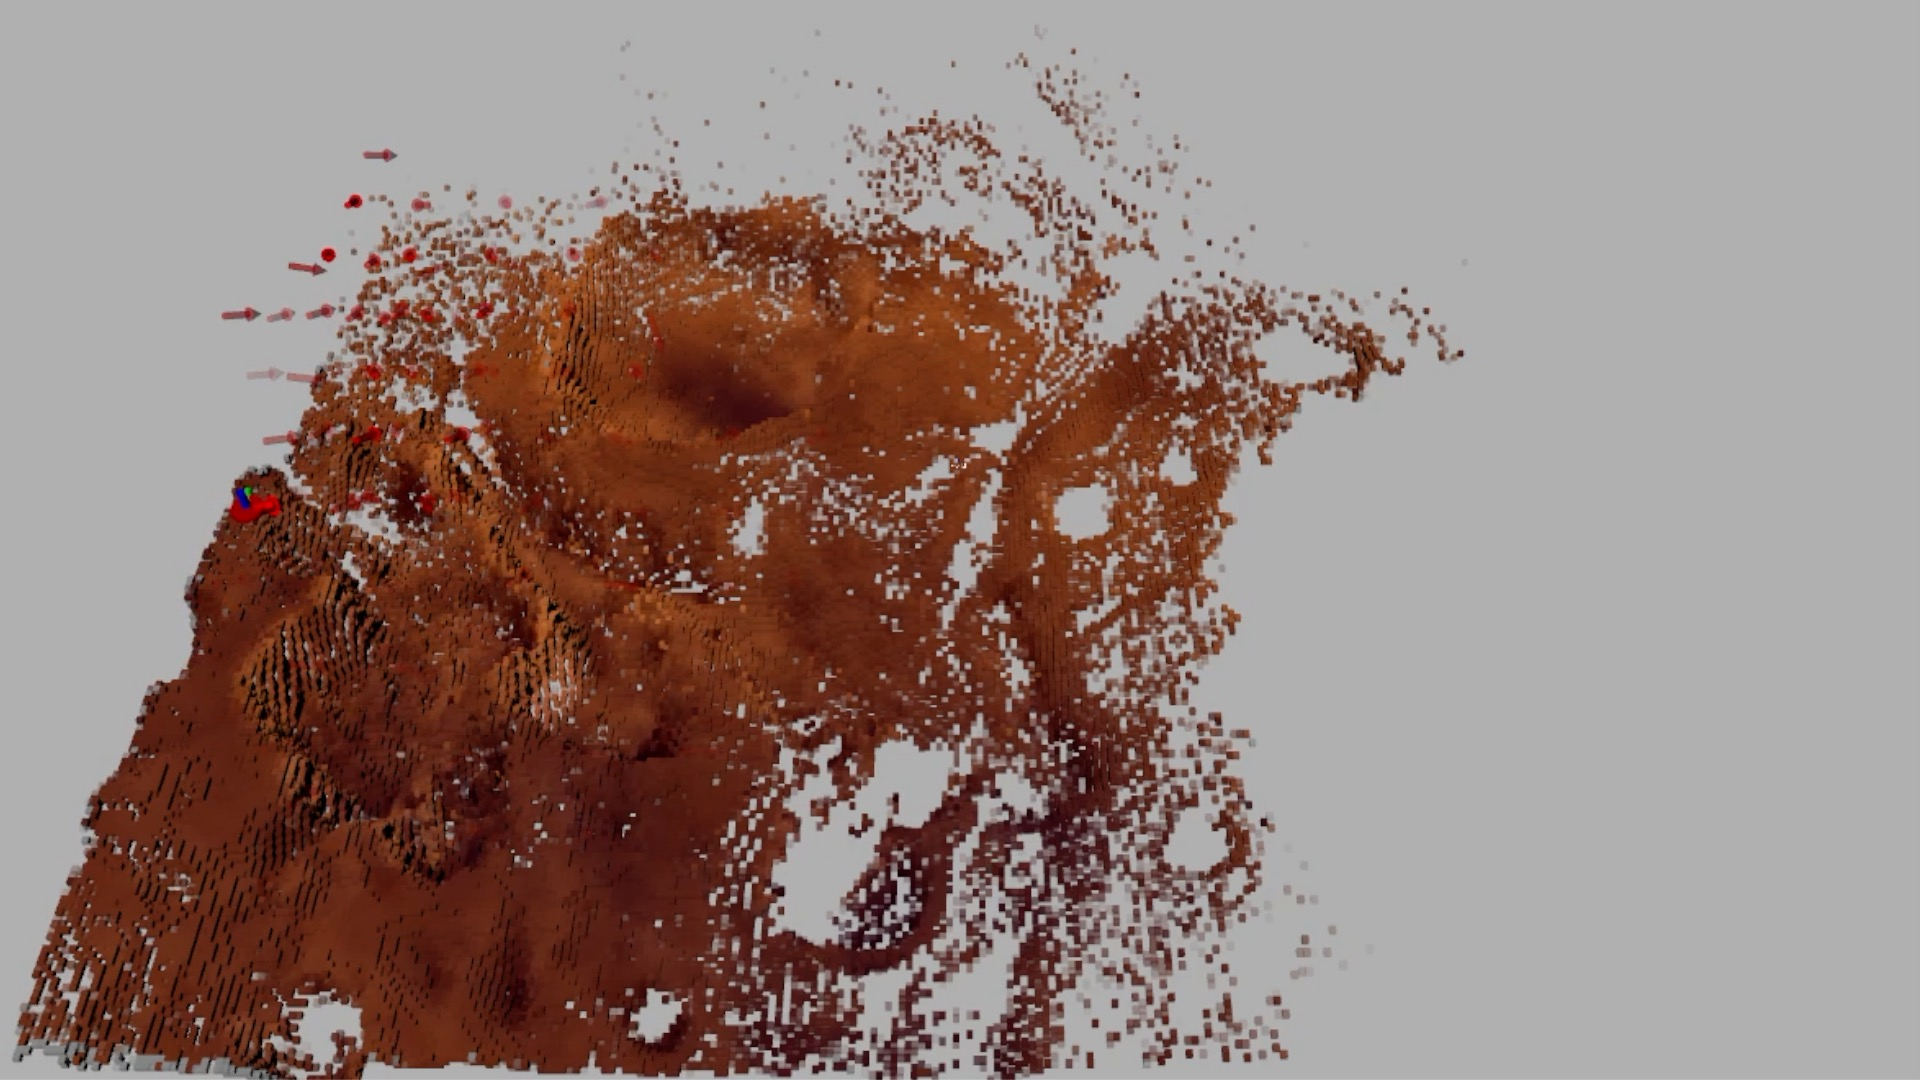
\includegraphics[height=0.5\textwidth]{FullMarsMap2min.jpg}
        		\caption{$2$ min}
		\vspace*{0.025\textwidth}
    	\end{subfigure}
    	\begin{subfigure}[t]{0.49\columnwidth}
           	\centering
          	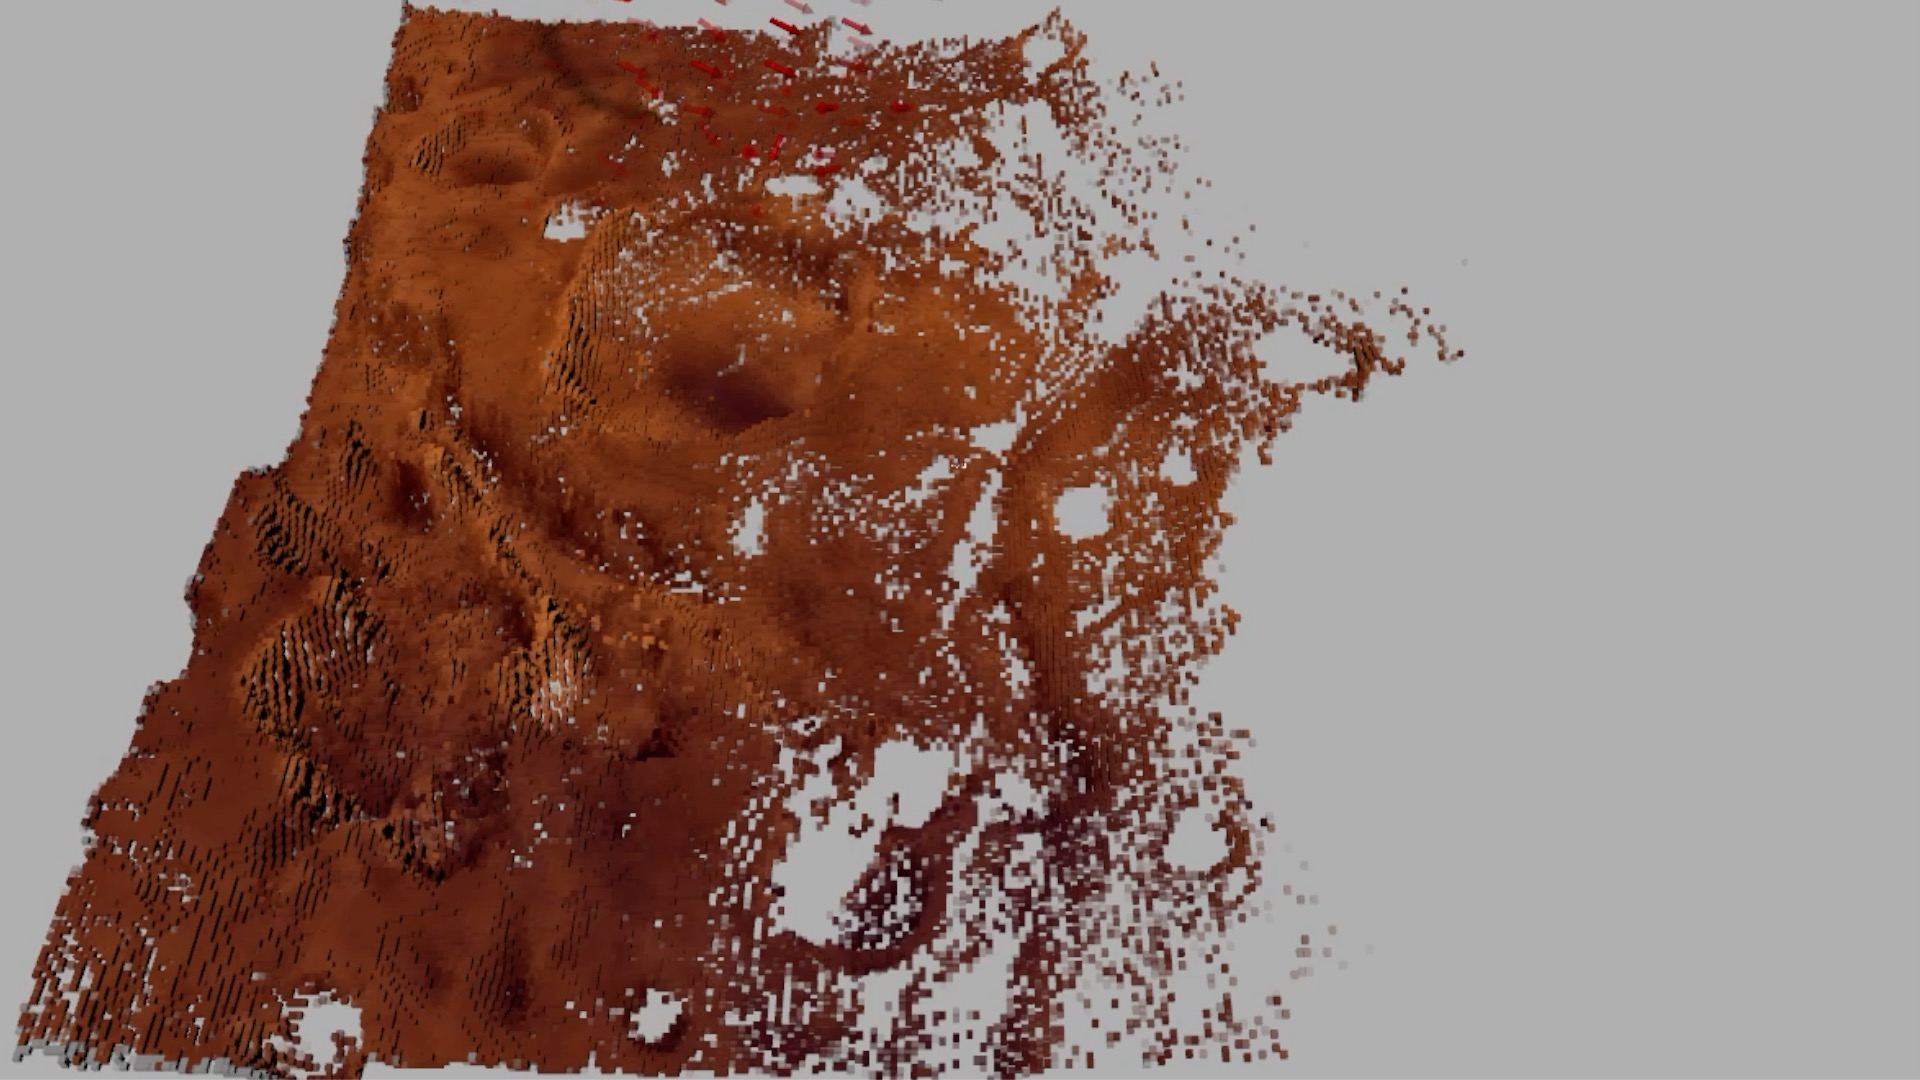
\includegraphics[height=0.5\textwidth]{FullMarsMap3min.jpg}
        		\caption{$3$ min}
		\vspace*{0.025\textwidth}
    	\end{subfigure}
	\centering
	\begin{subfigure}[t]{0.49\columnwidth}
           	\centering
          	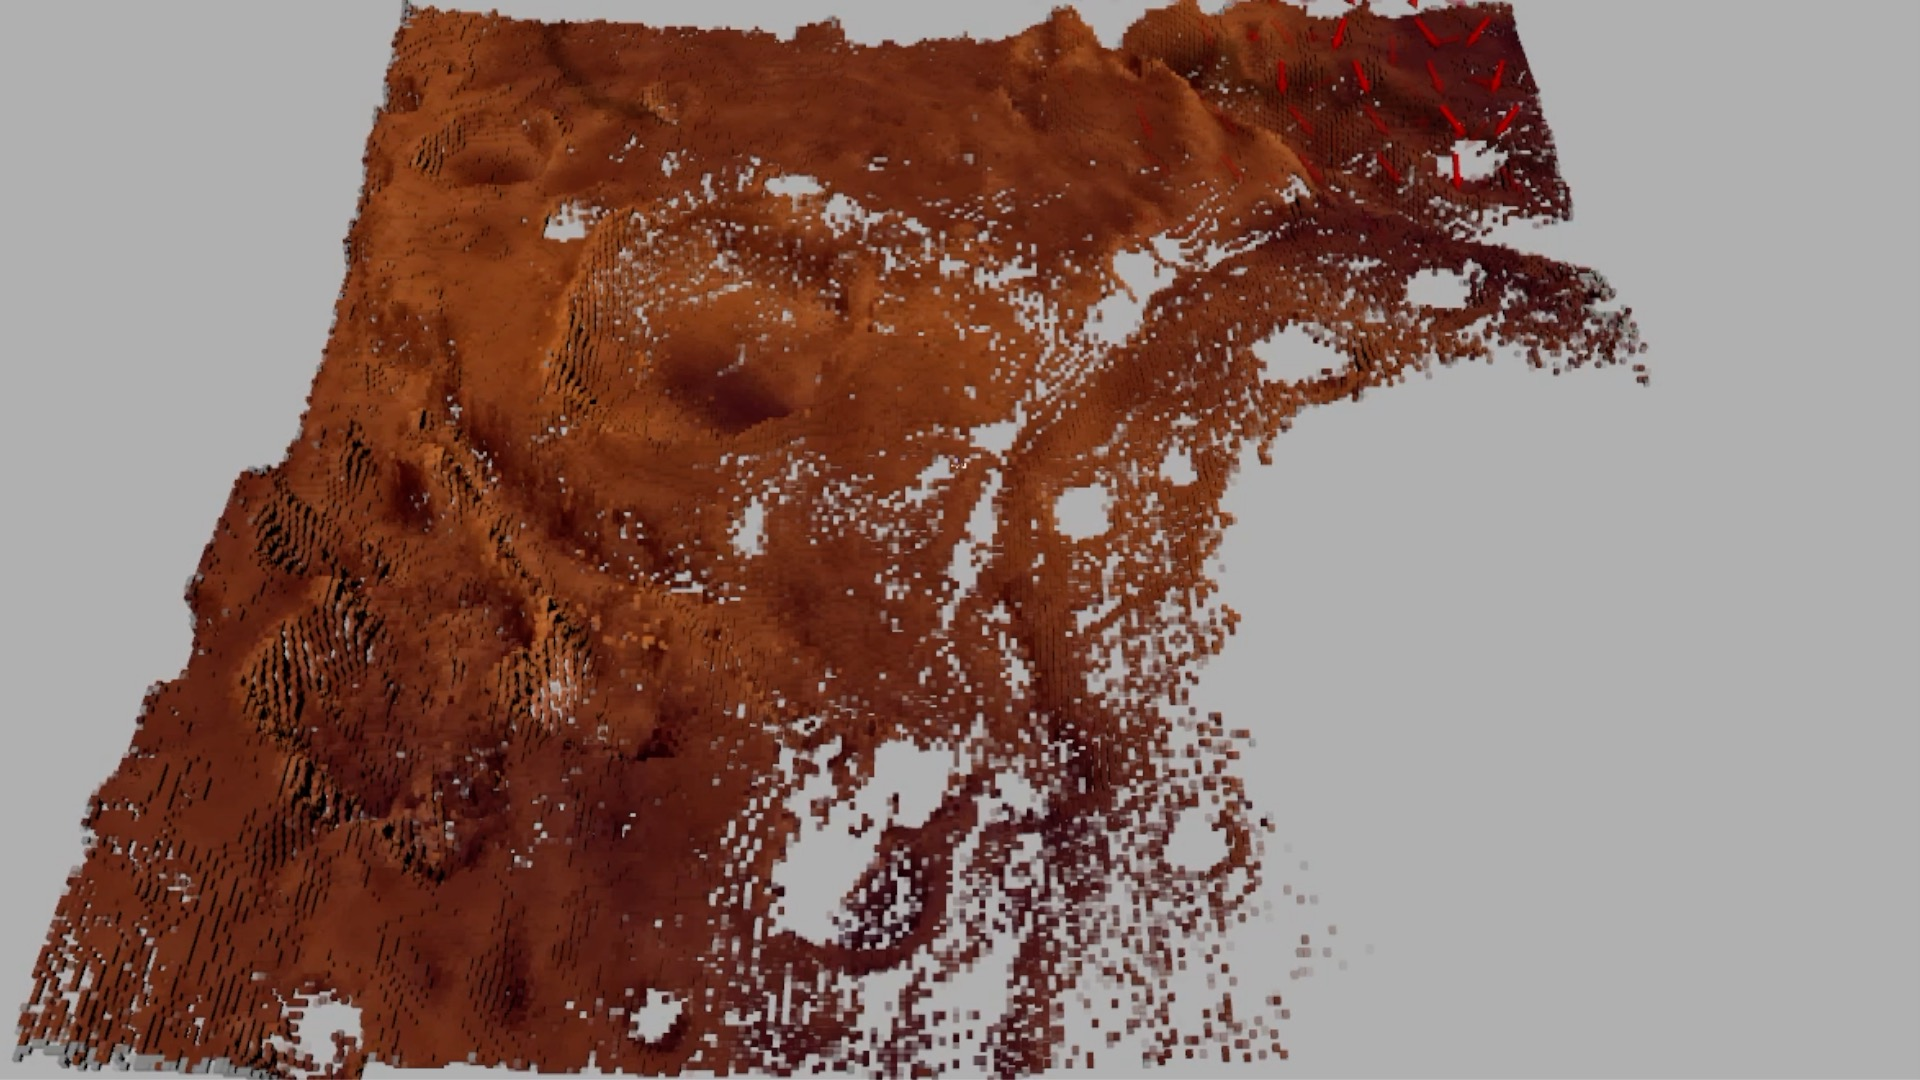
\includegraphics[height=0.5\textwidth]{FullMarsMap4min.jpg}
        		\caption{$4$ min}
		\vspace*{0.025\textwidth}
    	\end{subfigure}
    	\begin{subfigure}[t]{0.49\columnwidth}
           	\centering
          	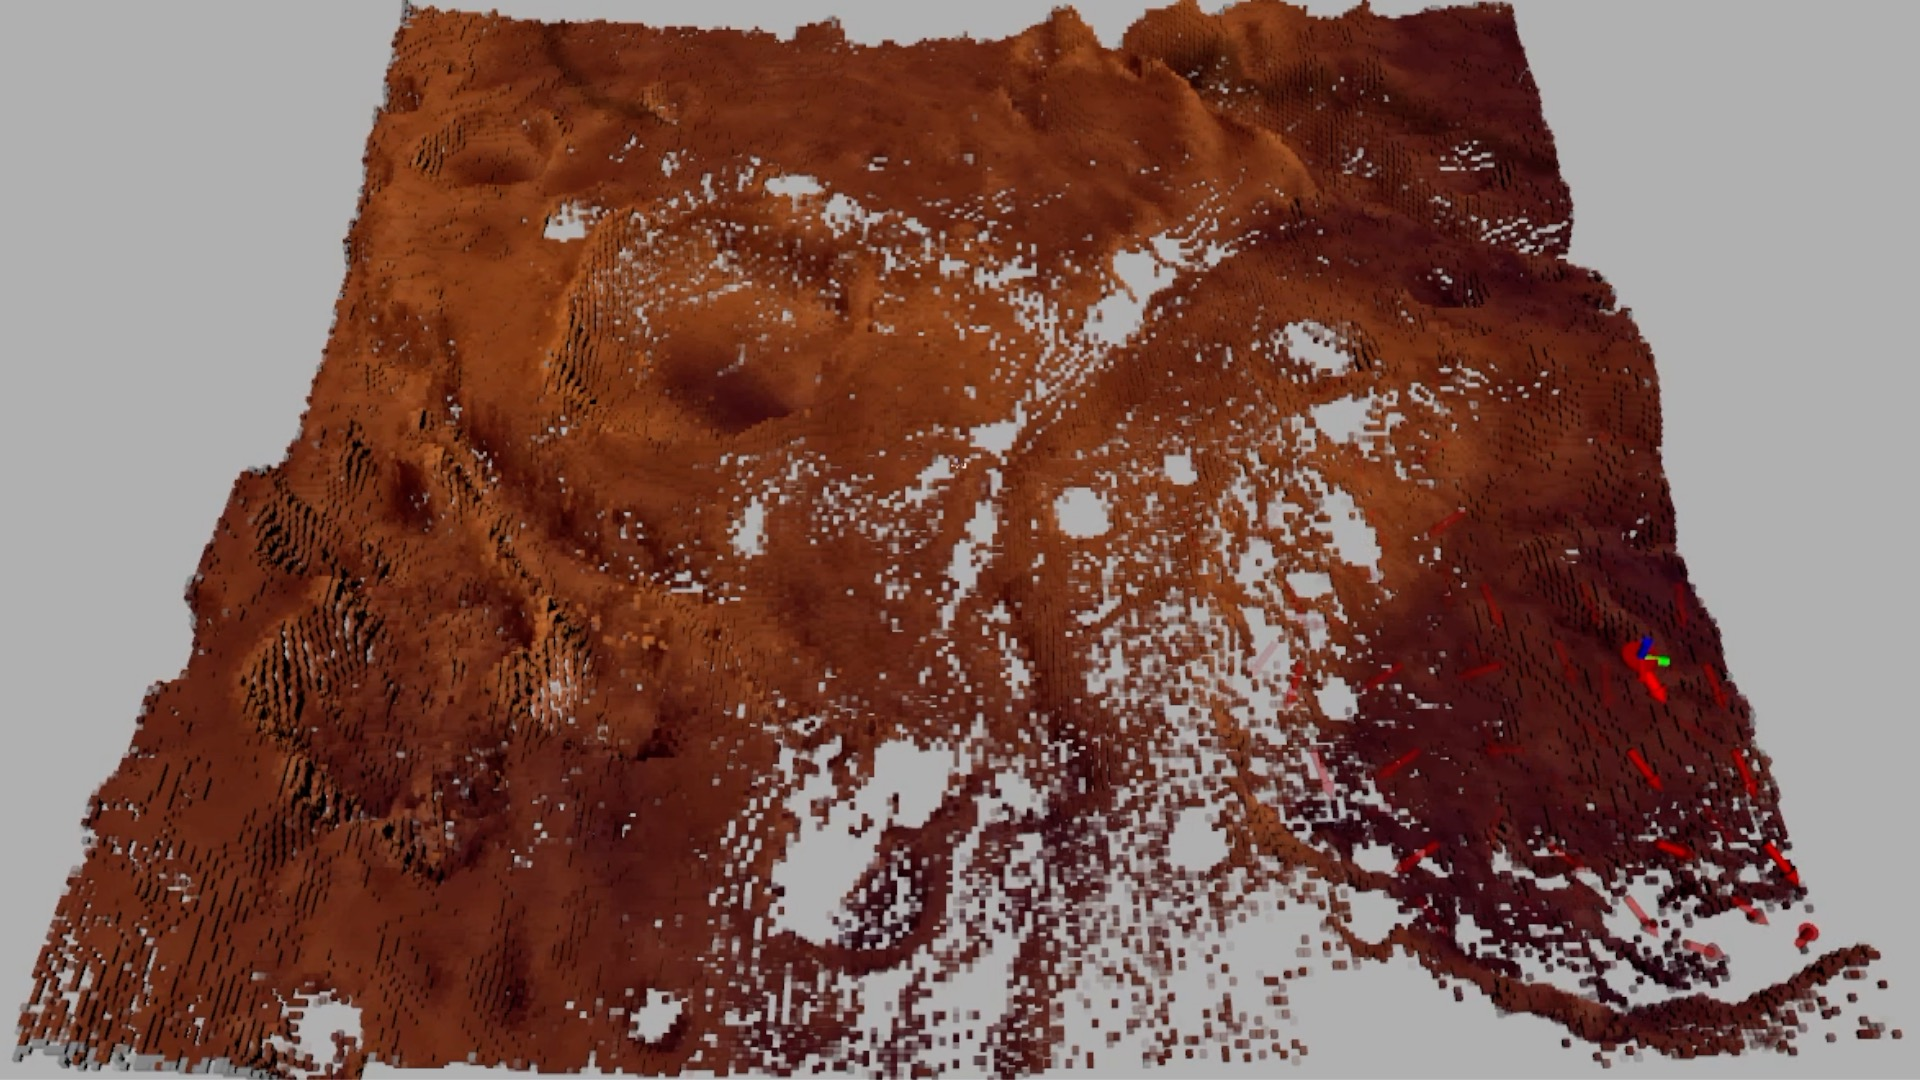
\includegraphics[height=0.5\textwidth]{FullMarsMap5min.jpg}
        		\caption{$5$ min}
		\vspace*{0.025\textwidth}
    	\end{subfigure}
	\centering
	\begin{subfigure}[t]{0.49\columnwidth}
           	\centering
          	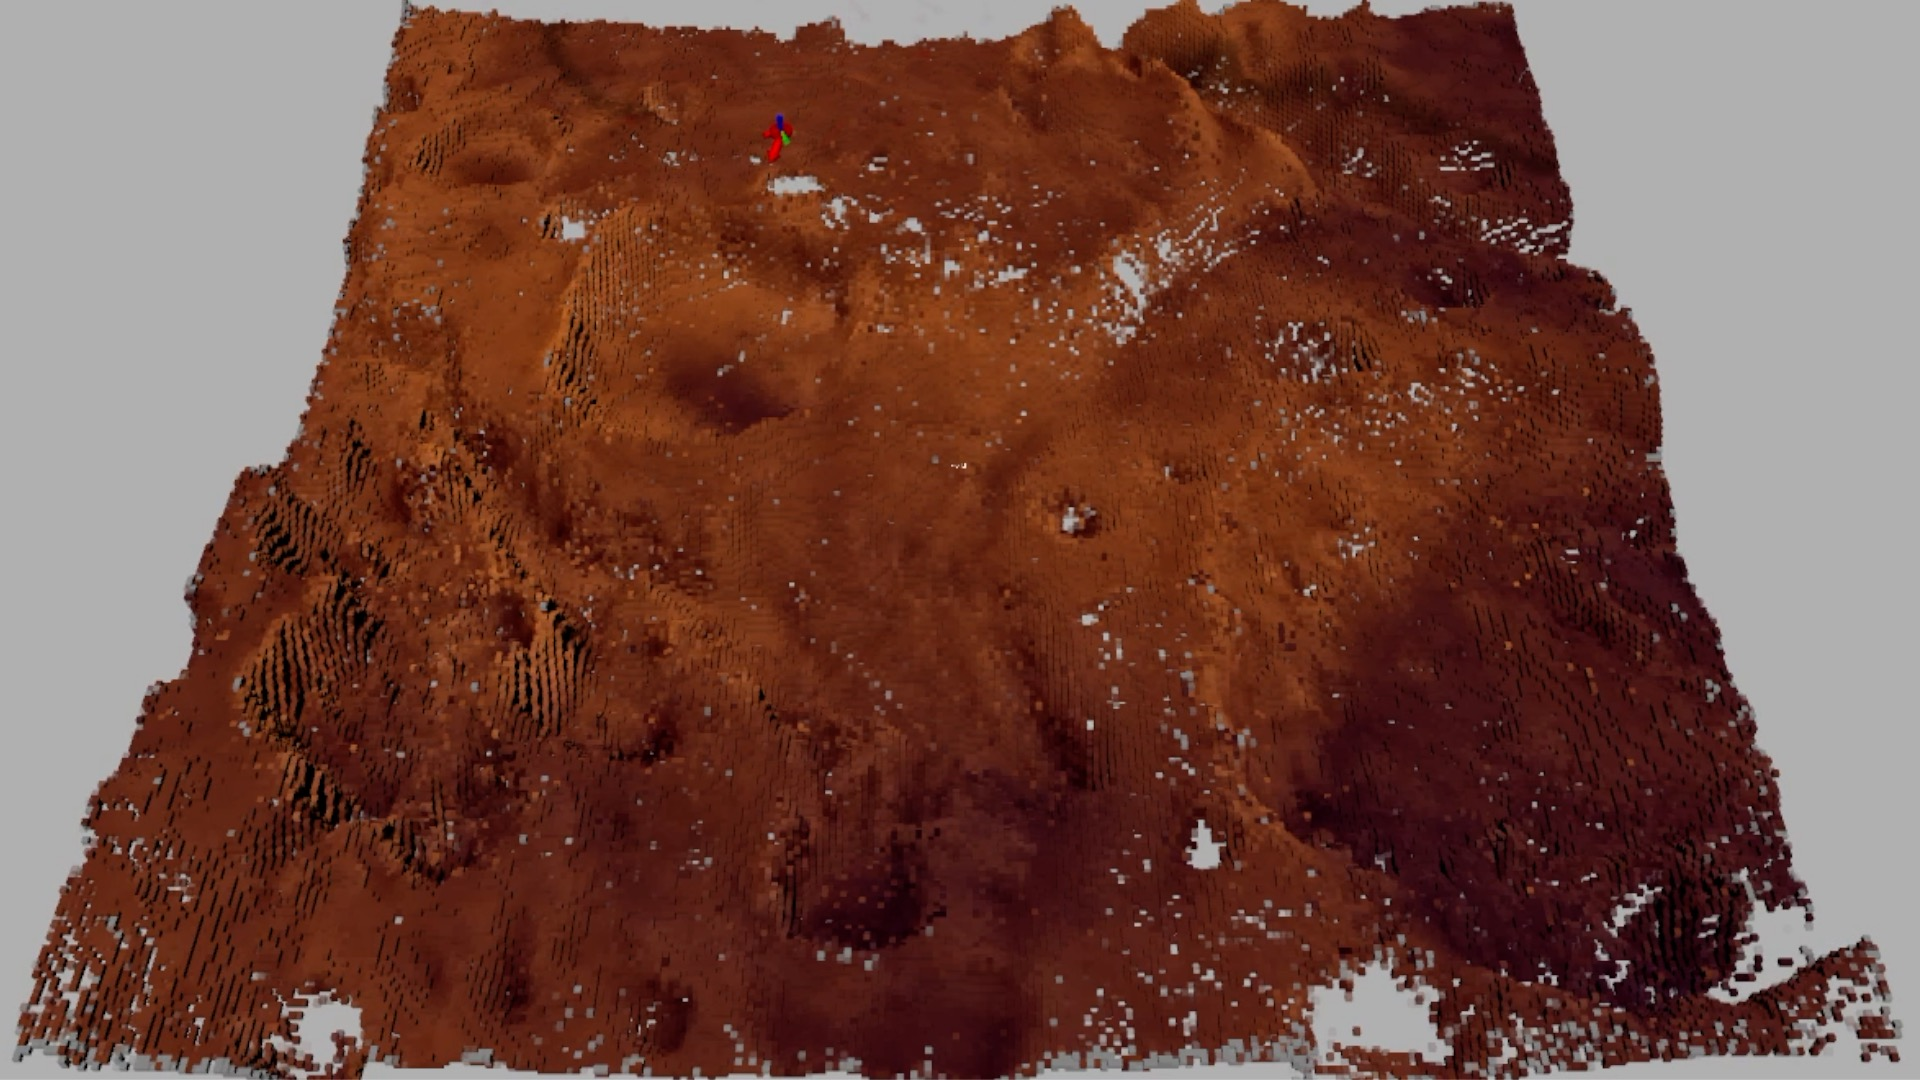
\includegraphics[height=0.5\textwidth]{FullMarsMap10min.jpg}
        		\caption{$10$ min}
		\vspace*{0.025\textwidth}
    	\end{subfigure}
    	\begin{subfigure}[t]{0.49\columnwidth}
           	\centering
          	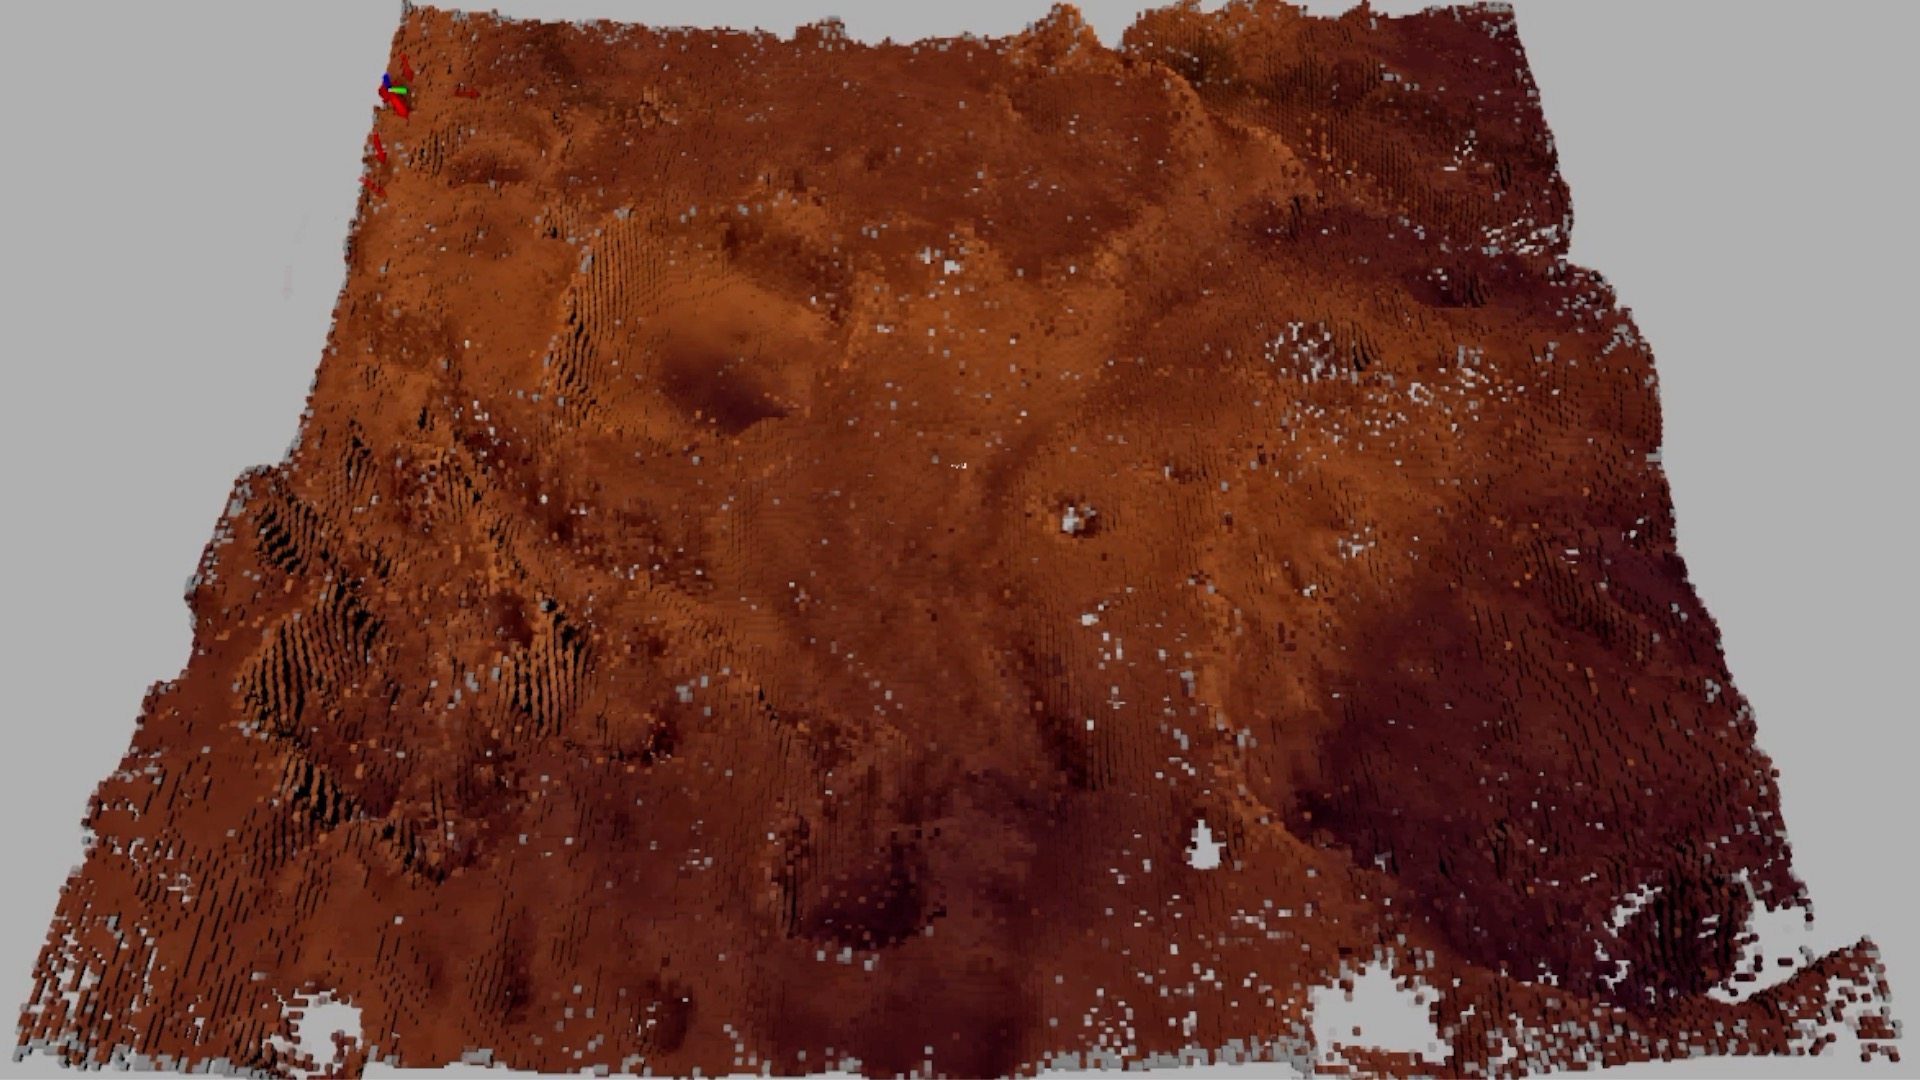
\includegraphics[height=0.5\textwidth]{FullMarsMap15min.jpg}
        		\caption{$15$ min}
		\vspace*{0.025\textwidth}
    	\end{subfigure}
\caption{In Case 1, the robot (red disk with arrow indicating laser direction) moves toward candidate poses (red arrows, more opaque for greater reward) based on expected entropy change of the 3D probabilistic occupancy grid map $m$ (cubes: greater opacity for greater occupancy probability) of the surface of Mars.}
\label{fig:mars3DogmCase1}
\end{figure}


\begin{figure}[!t]
	\centering
	\begin{subfigure}[t]{0.49\columnwidth}
           	\centering
          	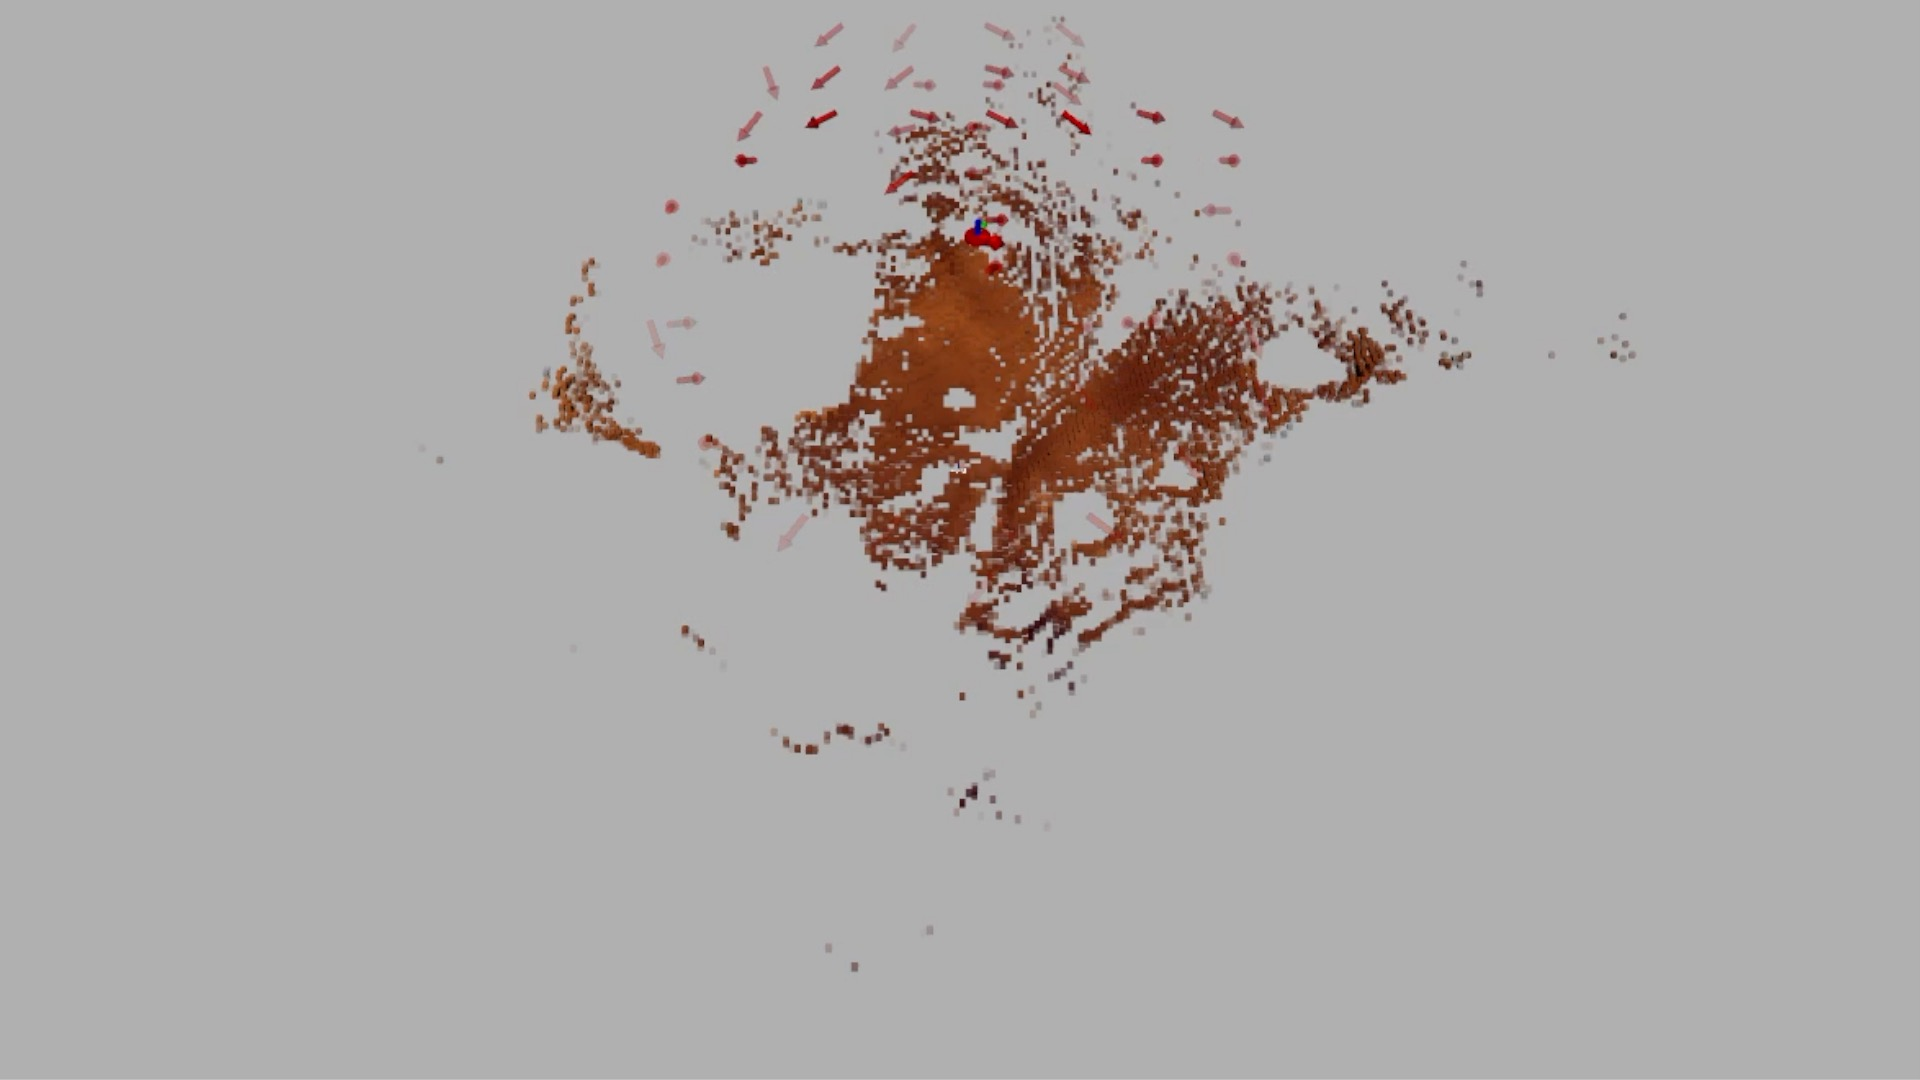
\includegraphics[height=0.5\textwidth]{RdcdMarsMap30sec.jpg}
        		\caption{$30$ sec}
		\vspace*{0.025\textwidth}
    	\end{subfigure}
    	\begin{subfigure}[t]{0.49\columnwidth}
           	\centering
          	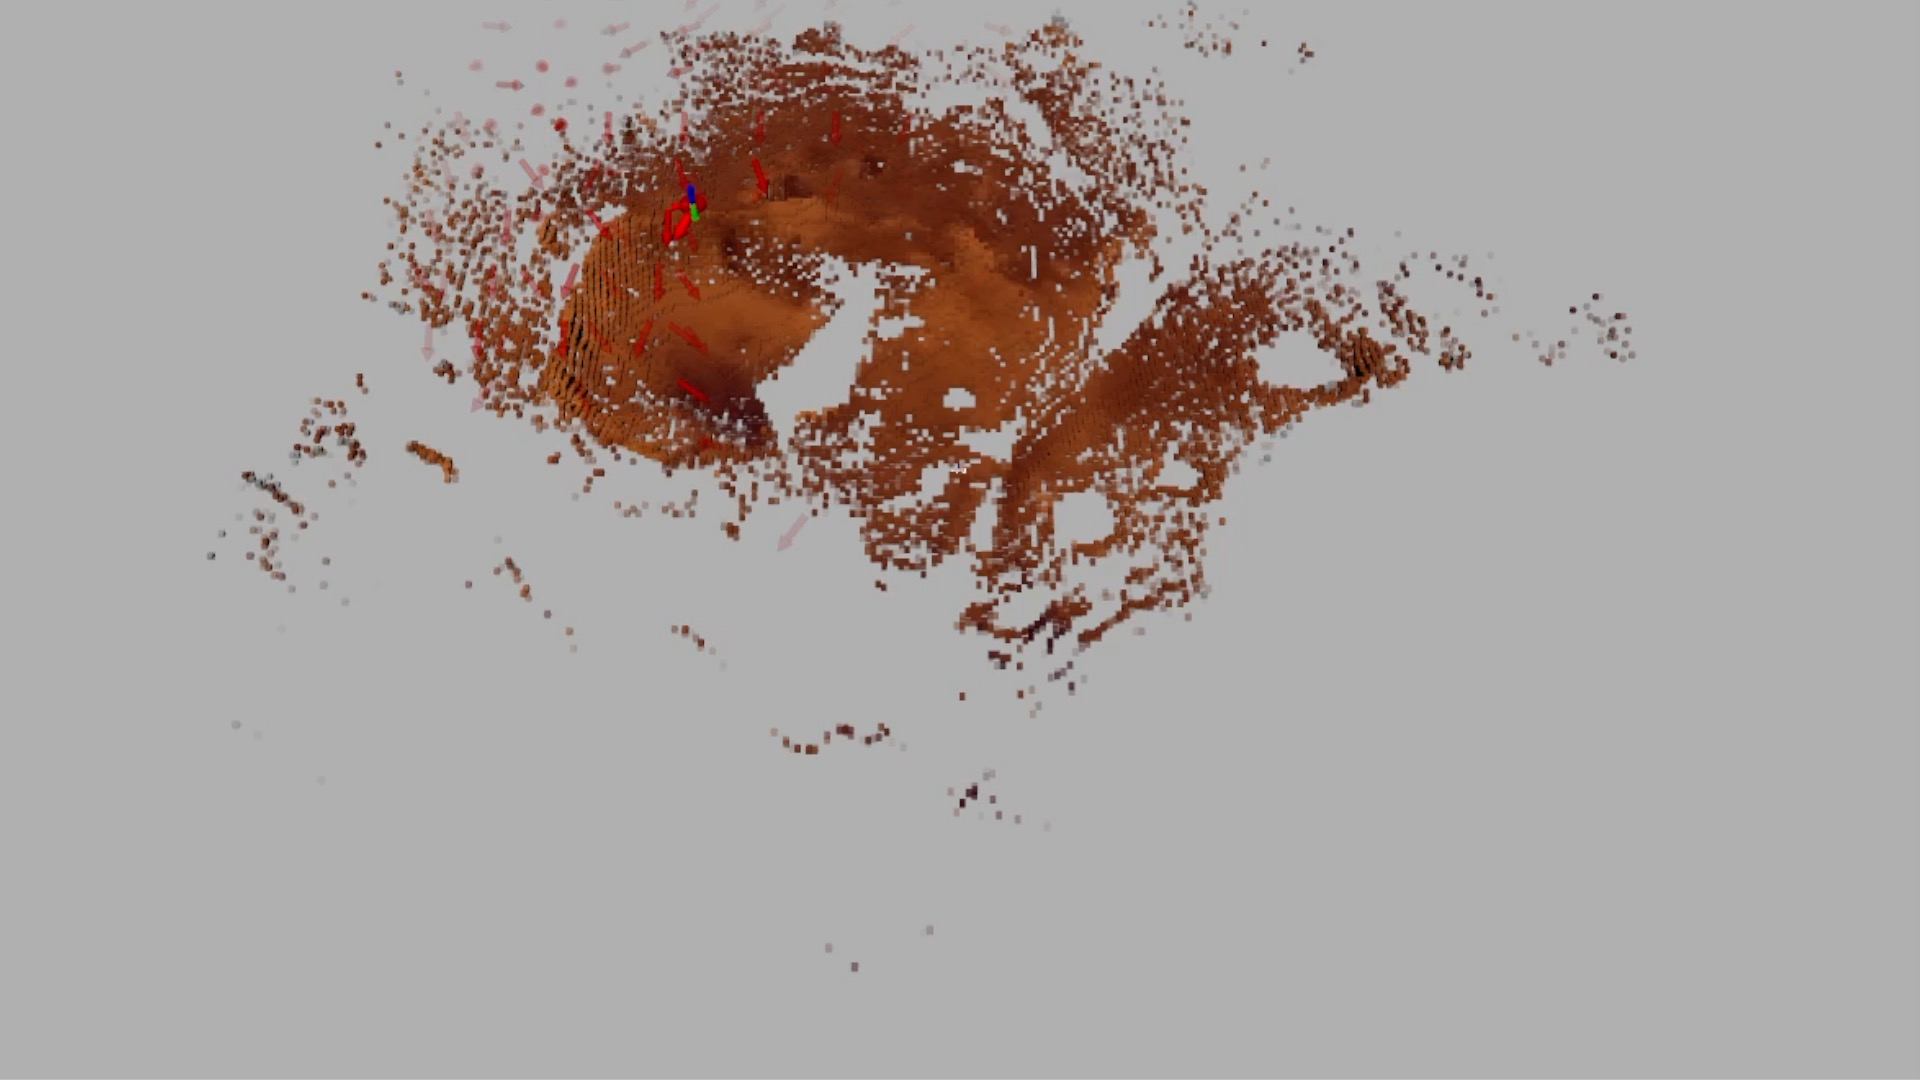
\includegraphics[height=0.5\textwidth]{RdcdMarsMap1min.jpg}
        		\caption{$1$ min}
		\vspace*{0.025\textwidth}
    	\end{subfigure}
	\centering
	\begin{subfigure}[t]{0.49\columnwidth}
           	\centering
          	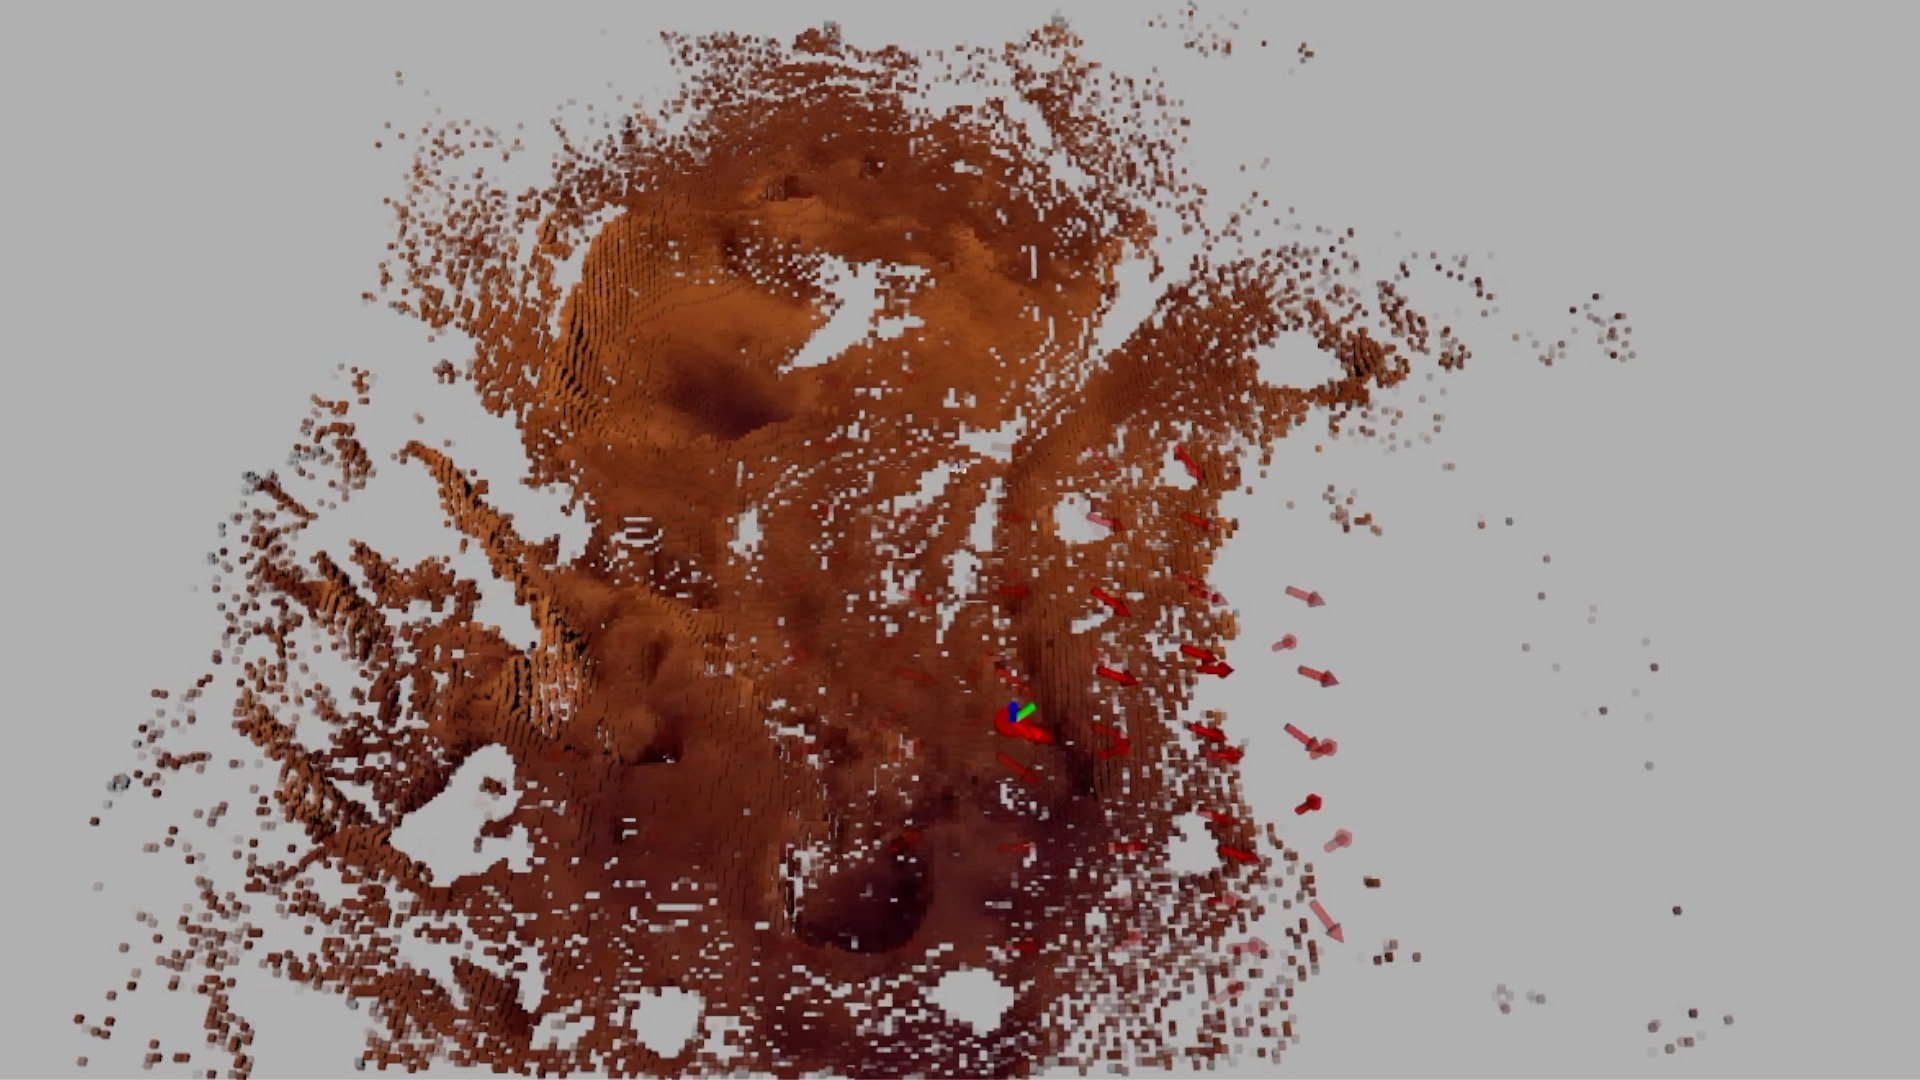
\includegraphics[height=0.5\textwidth]{RdcdMarsMap2min.jpg}
        		\caption{$2$ min}
		\vspace*{0.025\textwidth}
    	\end{subfigure}
    	\begin{subfigure}[t]{0.49\columnwidth}
           	\centering
          	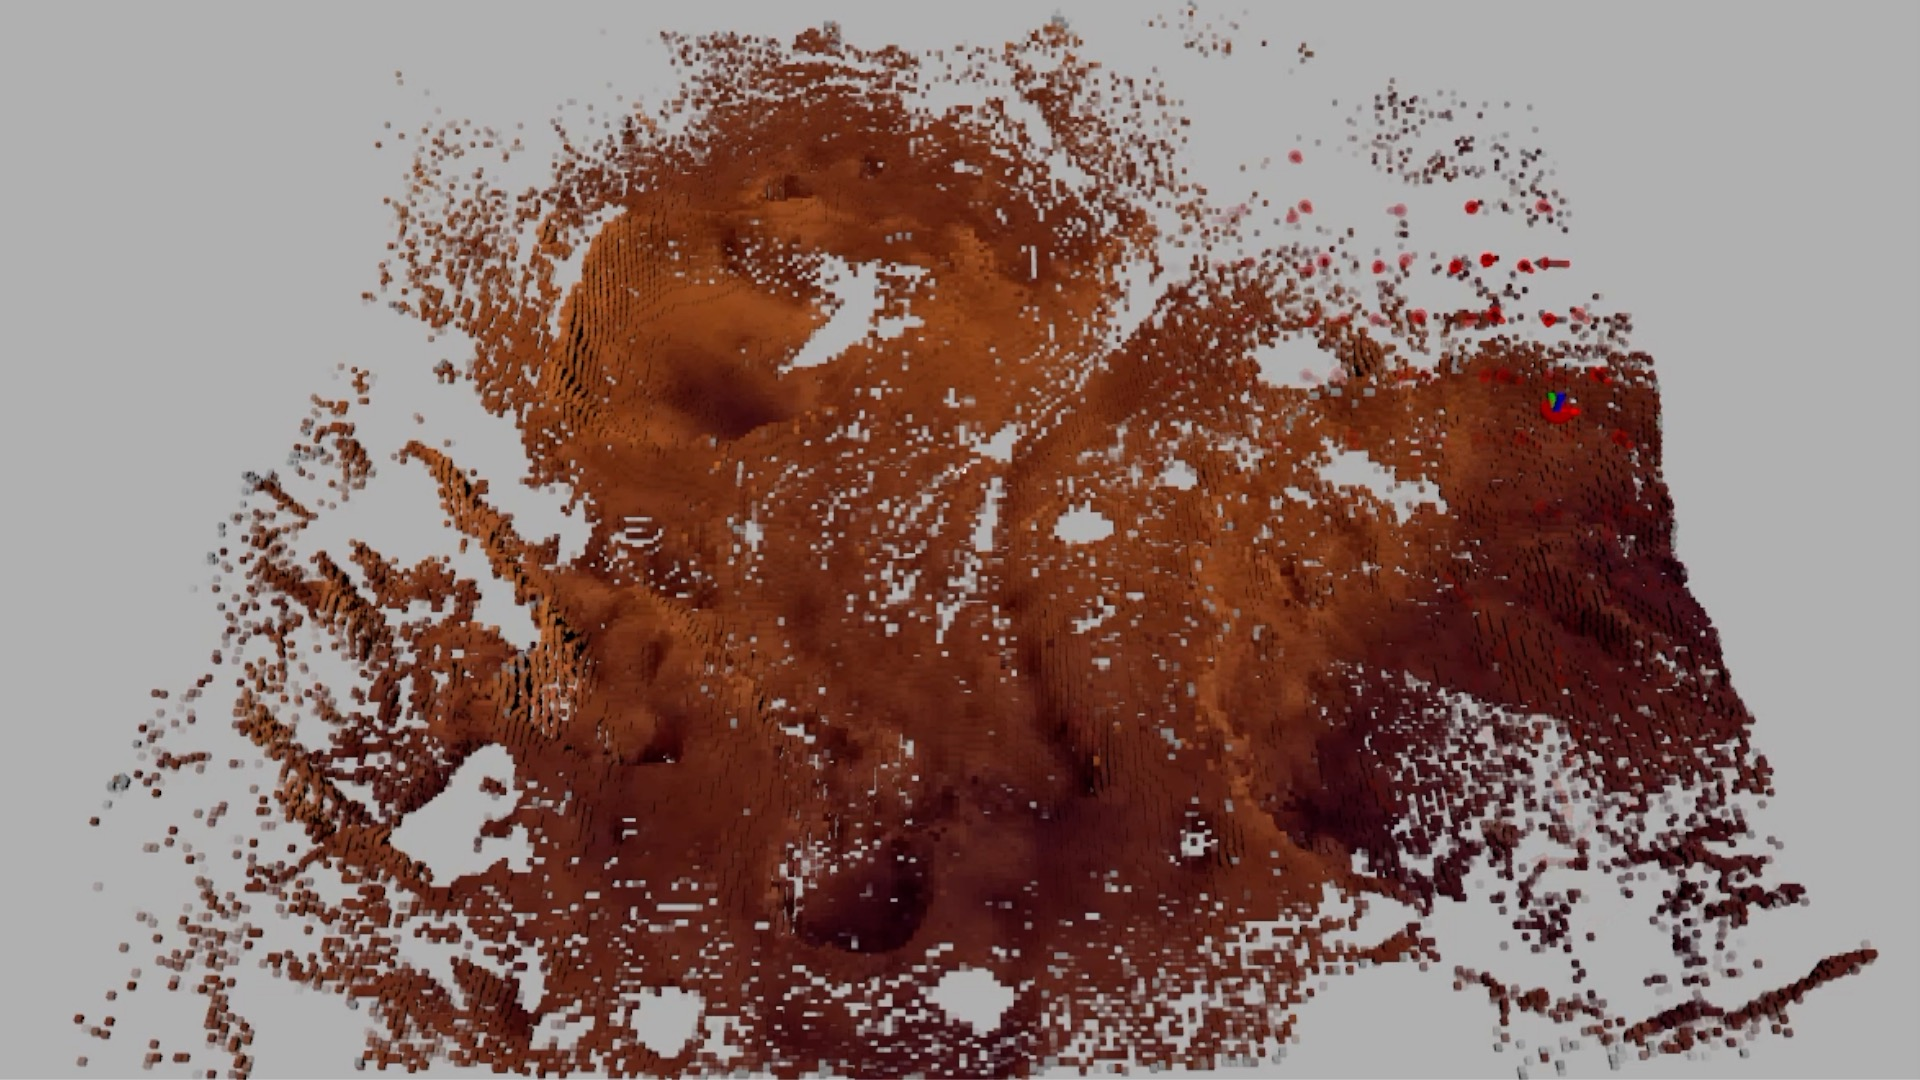
\includegraphics[height=0.5\textwidth]{RdcdMarsMap3min.jpg}
        		\caption{$3$ min}
		\vspace*{0.025\textwidth}
    	\end{subfigure}
	\centering
	\begin{subfigure}[t]{0.49\columnwidth}
           	\centering
          	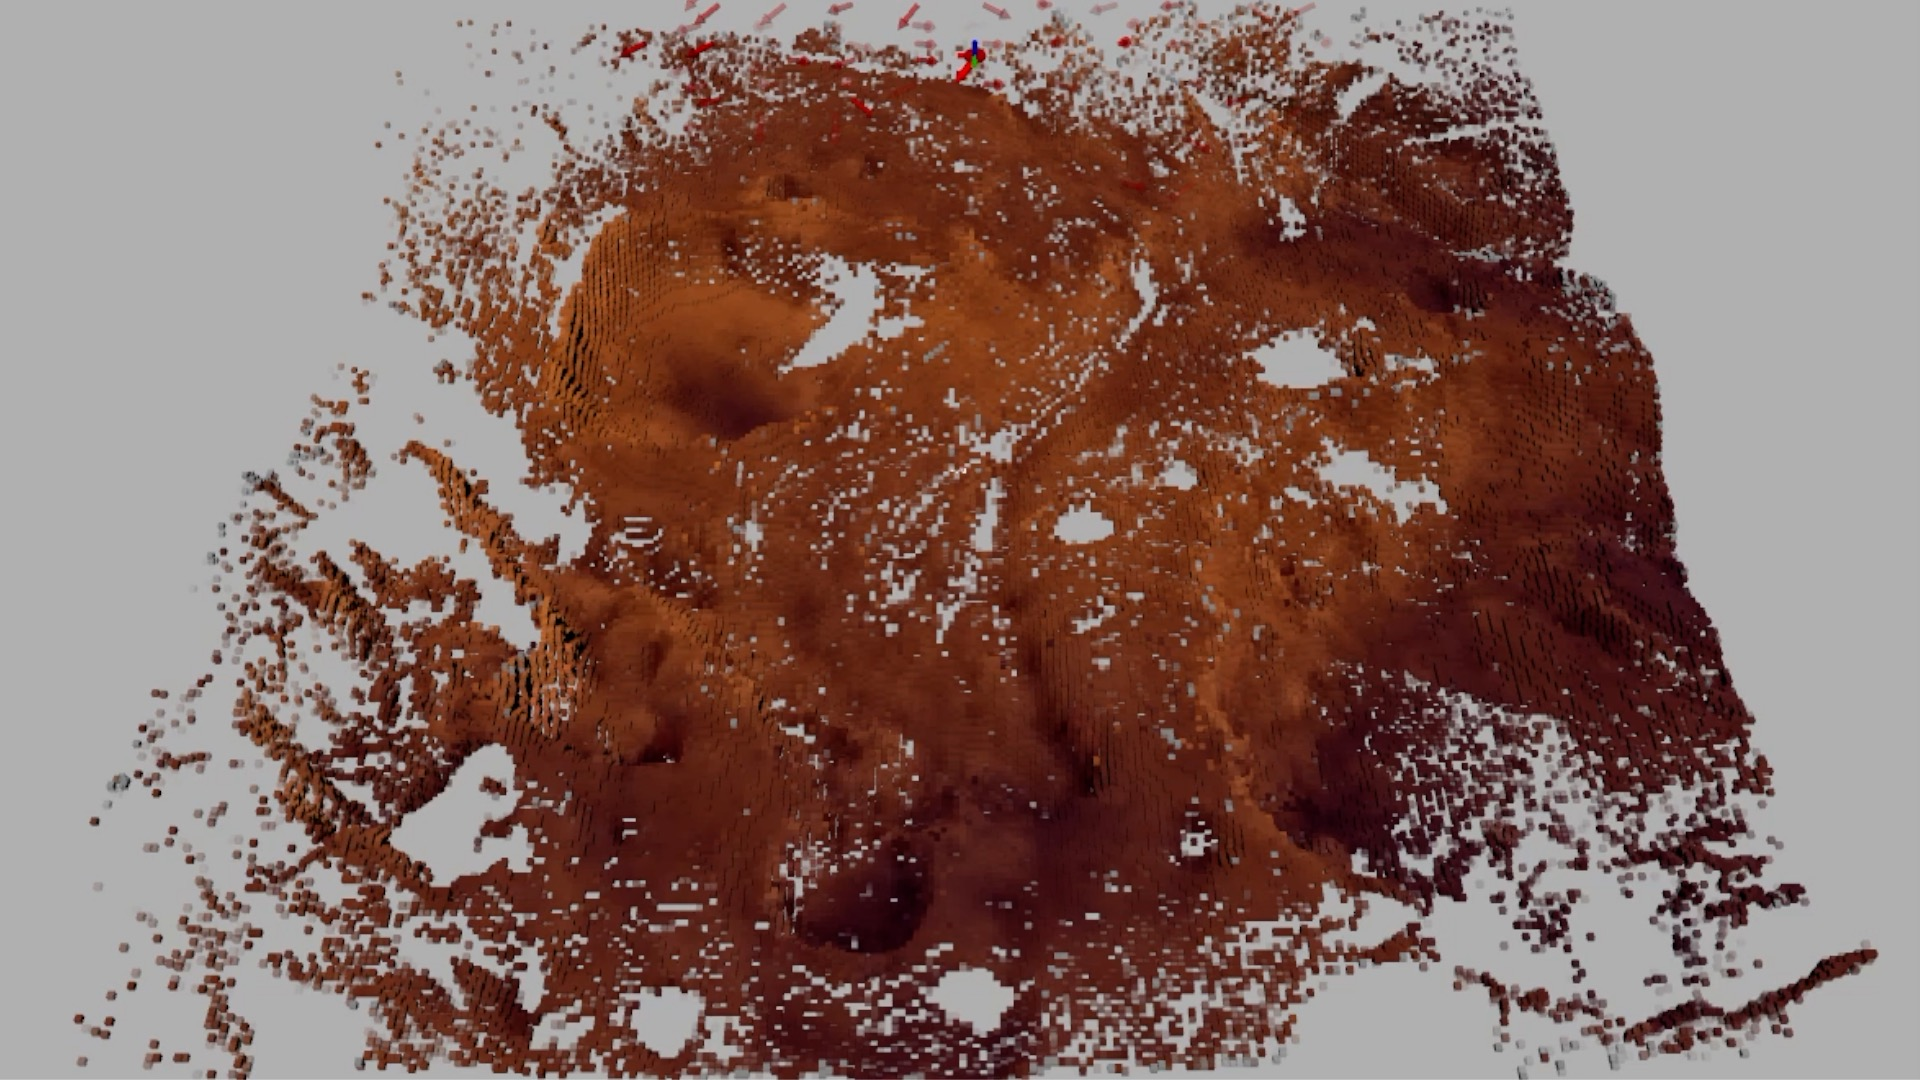
\includegraphics[height=0.5\textwidth]{RdcdMarsMap4min.jpg}
        		\caption{$4$ min}
		\vspace*{0.025\textwidth}
    	\end{subfigure}
    	\begin{subfigure}[t]{0.49\columnwidth}
           	\centering
          	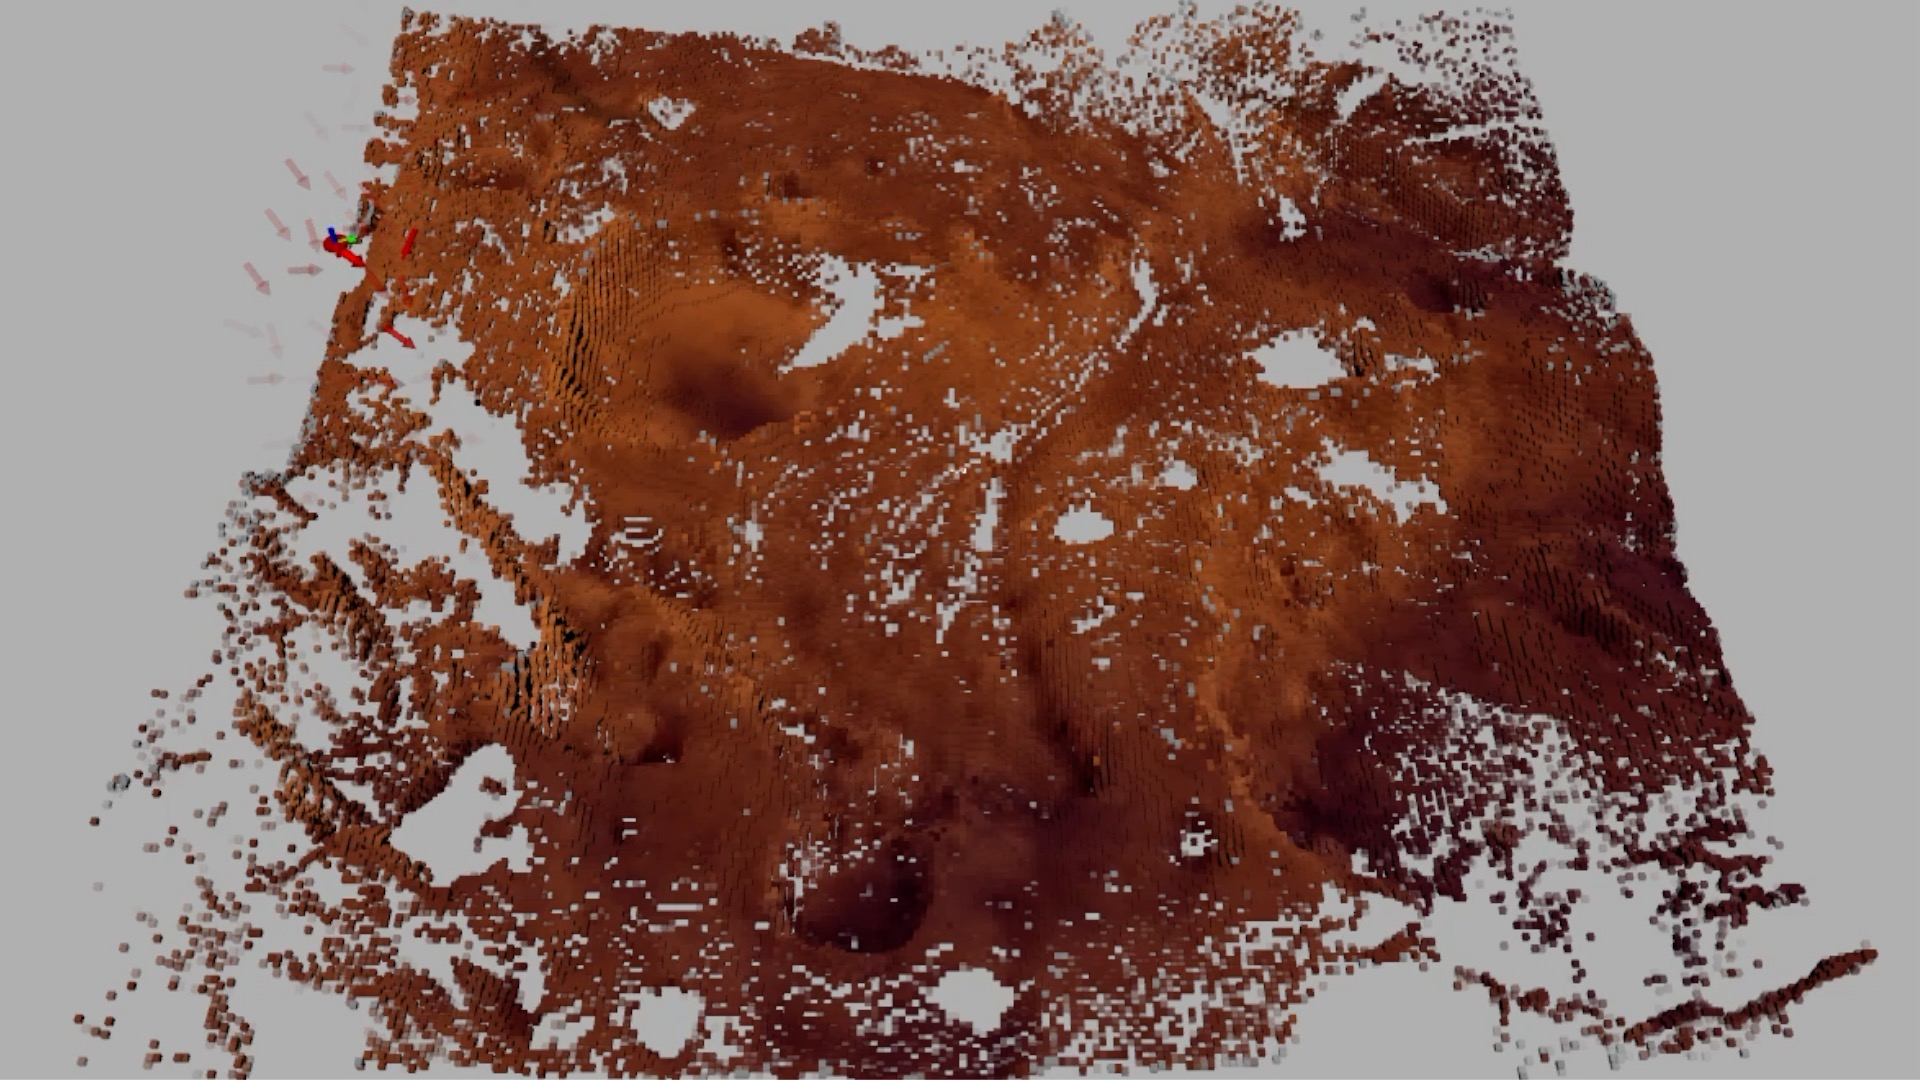
\includegraphics[height=0.5\textwidth]{RdcdMarsMap5min.jpg}
        		\caption{$5$ min}
		\vspace*{0.025\textwidth}
    	\end{subfigure}
	\centering
	\begin{subfigure}[t]{0.49\columnwidth}
           	\centering
          	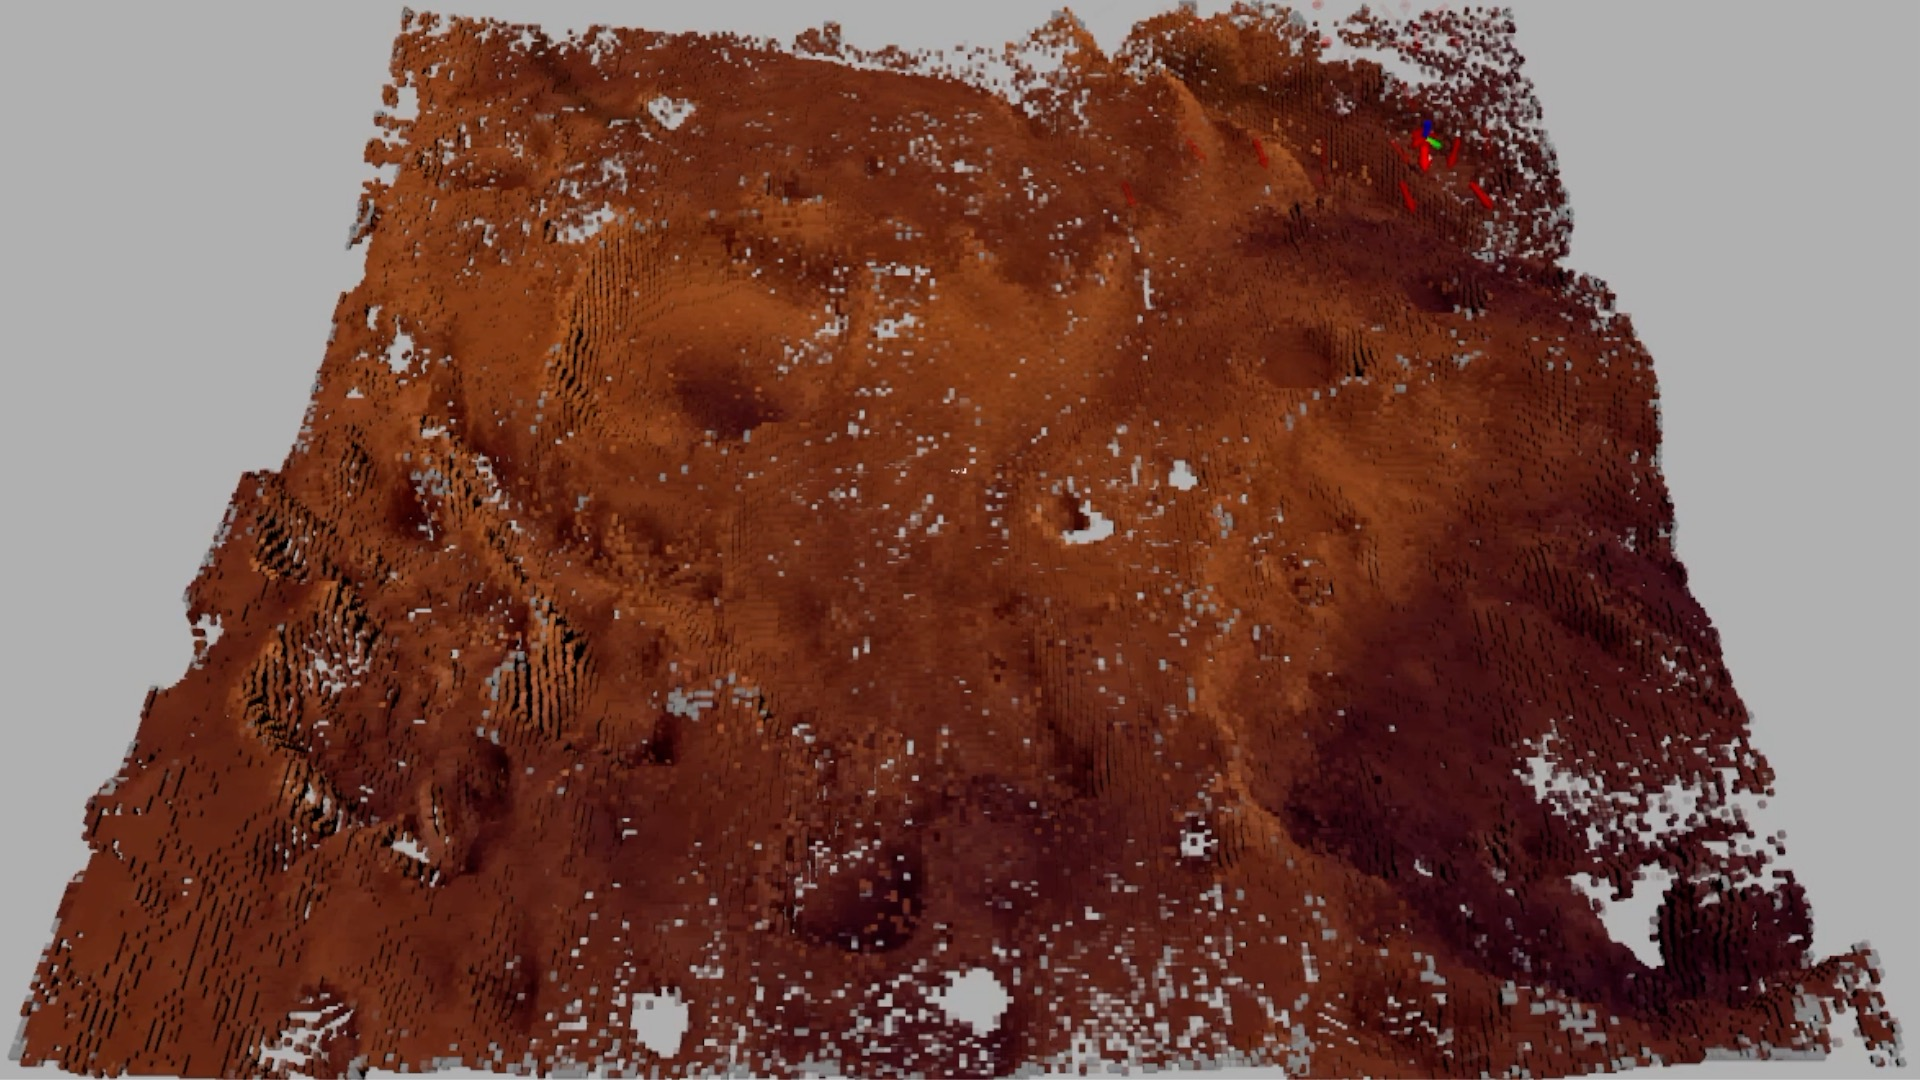
\includegraphics[height=0.5\textwidth]{RdcdMarsMap10min.jpg}
        		\caption{$10$ min}
		\vspace*{0.025\textwidth}
    	\end{subfigure}
    	\begin{subfigure}[t]{0.49\columnwidth}
           	\centering
          	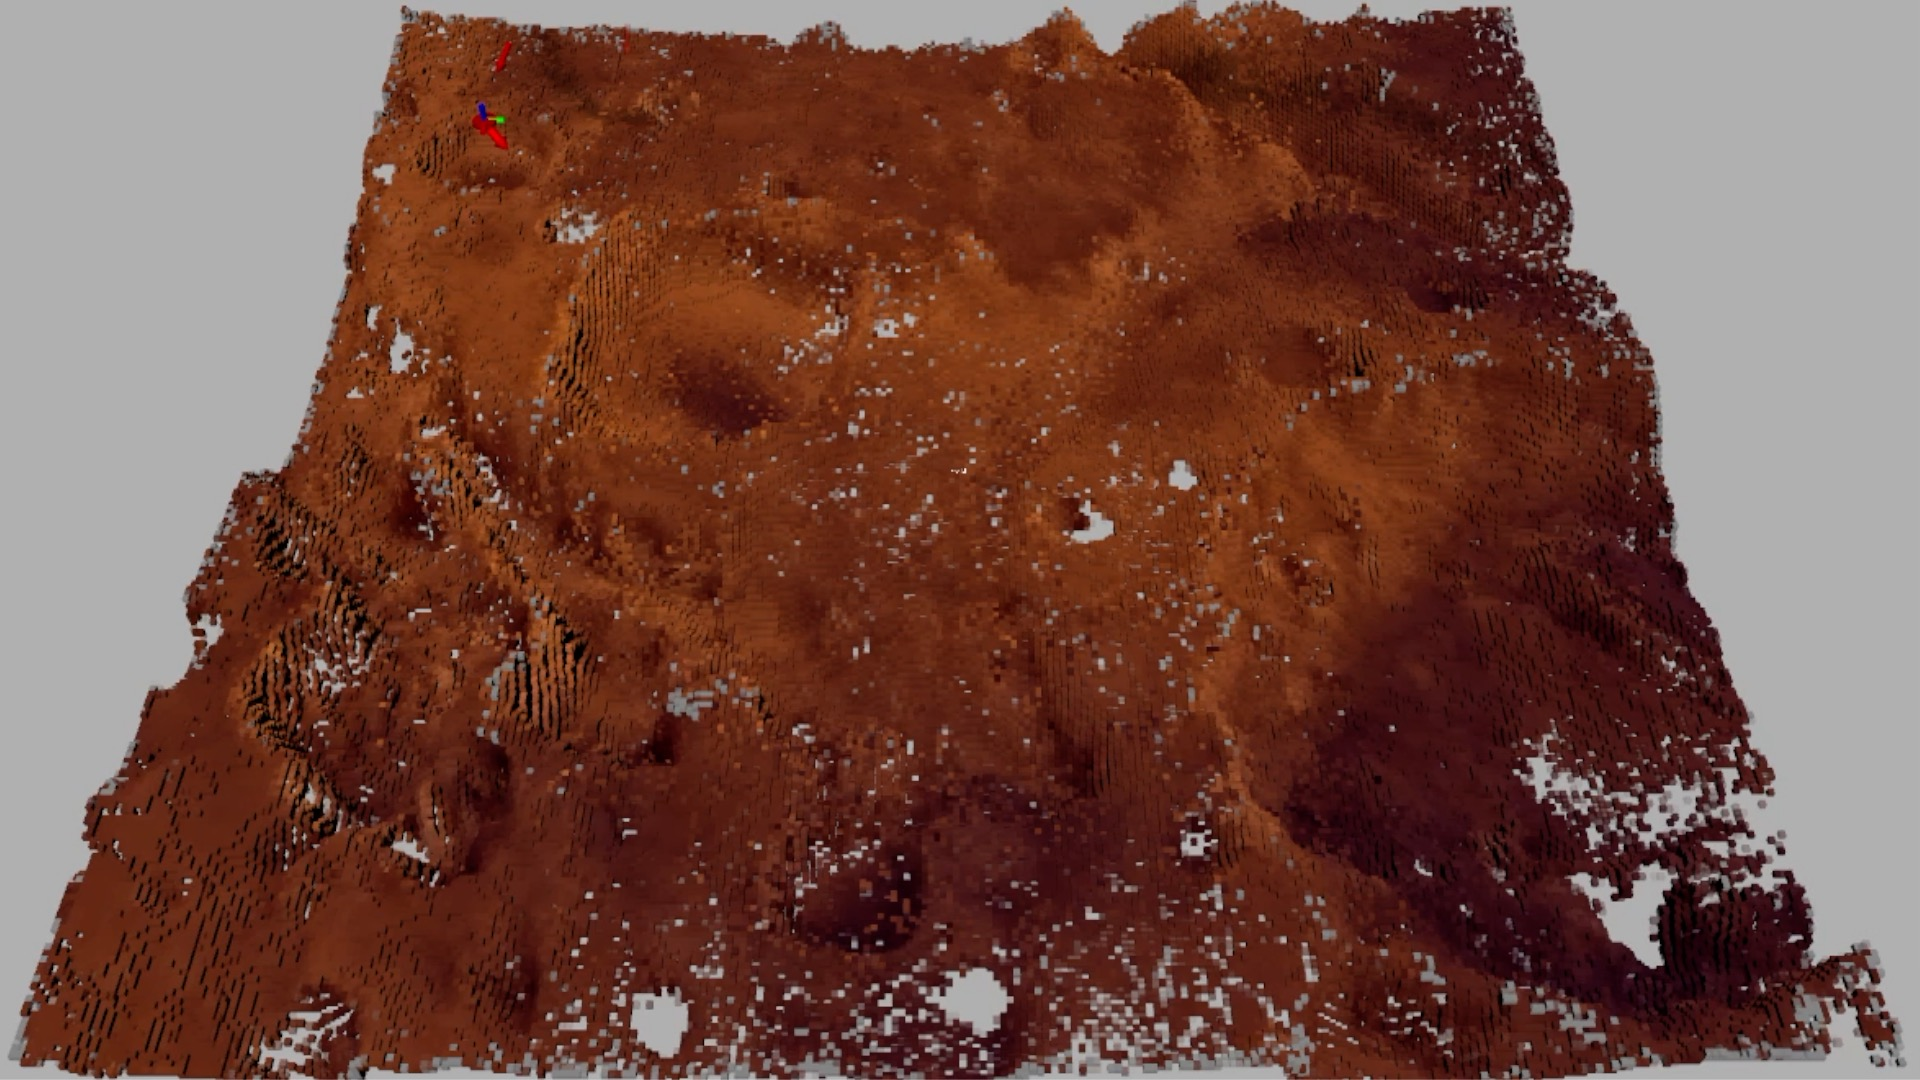
\includegraphics[height=0.5\textwidth]{RdcdMarsMap15min.jpg}
        		\caption{$15$ min}
		\vspace*{0.025\textwidth}
    	\end{subfigure}
\caption{In Case 2, the robot (red disk with arrow indicating laser direction) generates a 3D probabilistic occupancy grid map $m$ (cubes: greater opacity for greater occupancy probability), which is used to generate a reduced map $m_\text{reduced}$ based on \refeqn{Proj3DMapComb}. The robot moves toward candidate poses (red arrows, more opaque for greater reward) based on expected entropy change of $m_\text{reduced}$. Using $m_\text{reduced}$ instead of $m$ for entropy calculation leads to faster exploration of new terrain, but this leaves some grid cells missing.}
\label{fig:mars3DogmCase2}
\end{figure}

\begin{figure}[!t]
	\centering
	\begin{subfigure}[t]{0.95\columnwidth}
           	\centering
          	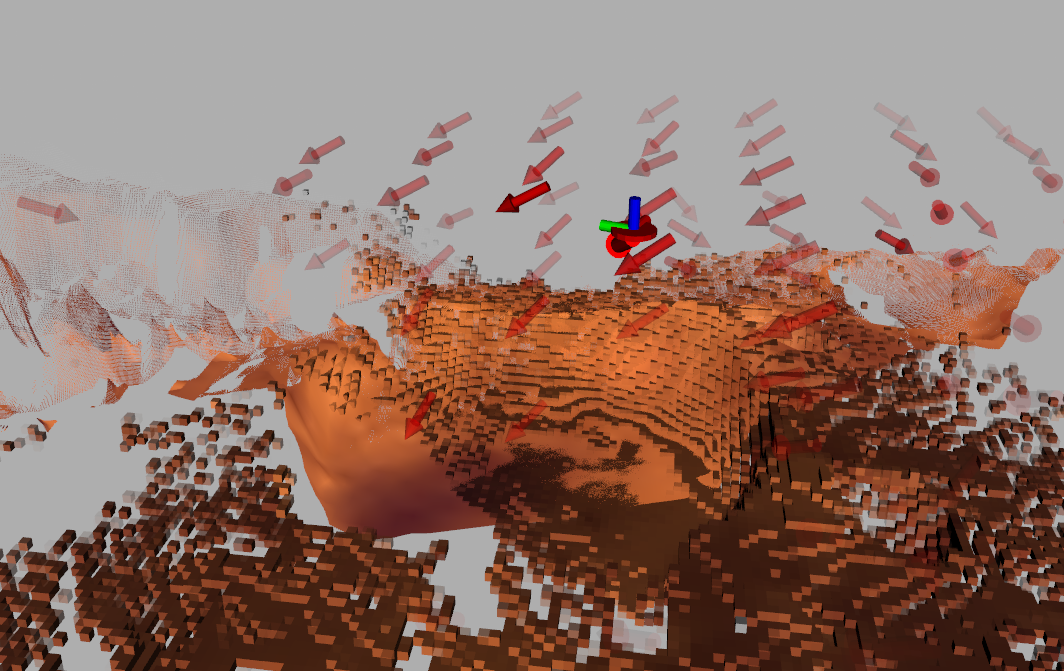
\includegraphics[width=\textwidth]{mars_closeup.png}
        		\caption{Full Map Cells and Sensor Scan}
		\vspace*{0.025\textwidth}
    	\end{subfigure}
	\centering
	\begin{subfigure}[t]{0.95\columnwidth}
           	\centering
          	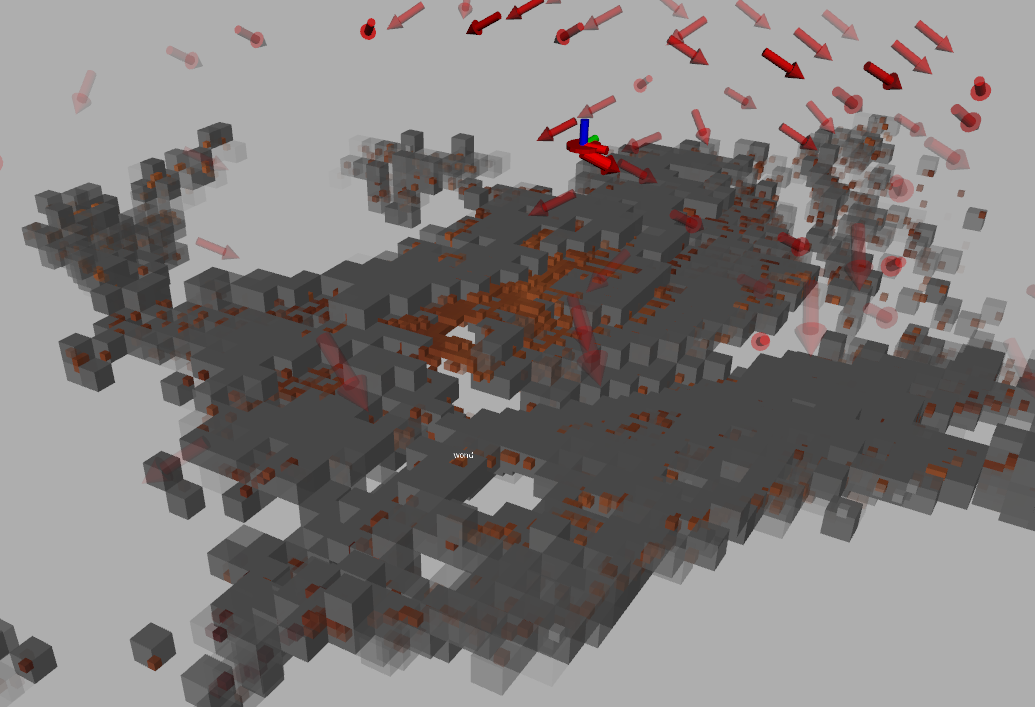
\includegraphics[width=\textwidth]{scitech_reducedCells.png}
        		\caption{Full Map and Reduced Map Cells}
		\vspace*{0.025\textwidth}
    	\end{subfigure}
\caption{The close-up images from the Case 2 trial show the candidate future poses (red arrows), where greater opacity represents a larger objective function of \refeqn{CandidateLocationOptimization}. In (a), we show the 3D scan with color corresponding to the surface of Mars. In (b), we overlay the full map $m$ (colored) with the reduced map $m_\text{reduced}$ (gray) from \refeqn{Proj3DMapComb}.}
\label{fig:marsZoomedIn}
>>>>>>> evan
\end{figure}


	\begin{figure}
		\centerline{
<<<<<<< HEAD
			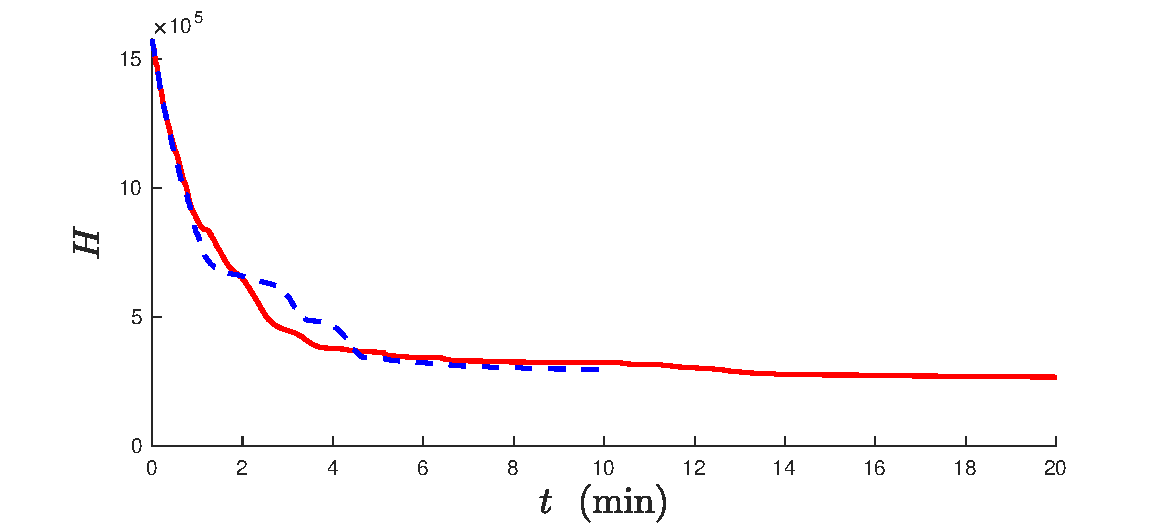
\includegraphics[width=0.6\columnwidth]{mars_H_comparison_flat.pdf}
		}
		\caption{The complete map entropy for Case 1 (red solid line) decreases at roughly the same rate as the reduced map entropy for Case 2 (dashed blue line), but the complete map entropy highlights a few locations where entropy can decrease further, shown by lower entropy over the subsequent $10$ min.}
=======
			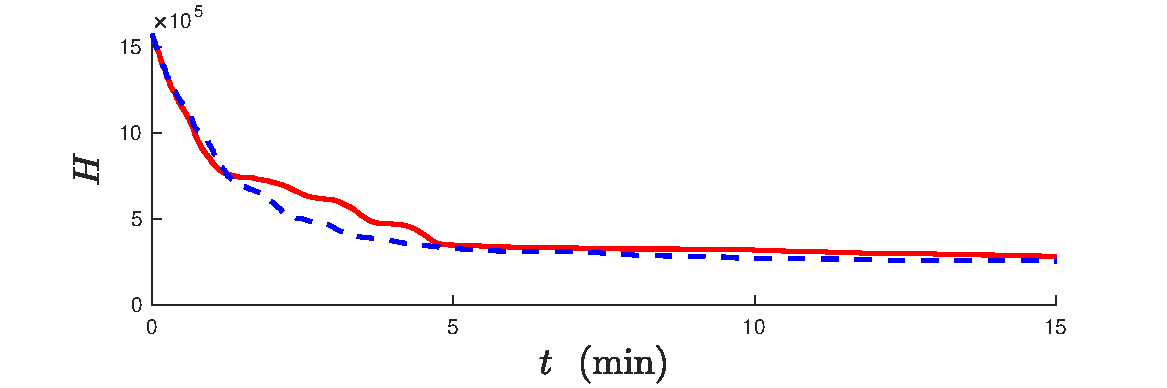
\includegraphics[width=0.6\columnwidth]{scitech_entropy_comparison_flat.pdf}
		}
		\caption{The complete map entropy for Case 1 (red solid line) decreases at roughly the same rate as the reduced map entropy for Case 2 (dashed blue line) toward the beginning. However, the expected entropy in Case 2 promotes actions toward unexplored territory, while the policy of Case 1 yields a more complete map before moving on to unexplored spaces.}
>>>>>>> evan
		\label{fig:mars3Dentropy}
	\end{figure}


In both cases, the robot built the 3D probabilistic map of the $2000$ cubic meter space composed of $4.74\times10^6$ grid cells. The maps were mostly complete within $10$ minutes. The $\tilde{\theta}=30\degree$ downward viewing angle captured the ground nicely, as candidate attitudes tended to direct the onboard sensor toward uncertain regions on the surface of Mars. The proposed approach provided collision-free mapping and autonomous exploration in real-time.

<<<<<<< HEAD
However, the choice of occupancy grid map used for entropy predictions introduced an interesting tradeoff. In Case 1, when the full probabilistic map $m$ was used in \refeqn{Iscan}, regions where the grid cells were partially-known were frequently reconsidered until the space was well-known. Conversely in Case 2, when $m_\text{reduced}$ was used instead, the robot repeatedly left spaces that were missing a few grid cells to visit new terrain. This is because $m_\text{reduced}$ had some cells with large occupancy probabilities based on \refeqn{Proj3DMapComb}, which allowed some grid cells of $m$ enclosed within a cell of $m_\text{reduced}$ to be uncertain. The exploration policy of Case 2 incorrectly assumed these regions were well-known. Ironically, this false assumption sometimes actually led to greater information gains when the vehicle moved on to unvisited terrain. Here, the exploration policy of Case 2 suspended operations once expected information gains were insignificant, which happened after about $10$ minutes. However with Case $1$, which used $m$ for computing expected entropy, the exploration continued for an additional $10$ minutes, overall decreasing total map entropy further, generating a more complete occupancy grid of the surface of Mars. 

In short, the proposed 3D probabilistic occupancy grid mapping and autonomous exploration were simulated successfully in real-time over the surface of Mars using ROS and Gazebo. Choosing $m$ for entropy predictions produced a more-complete map, but choosing $m_\text{reduced}$ was sometimes beneficial for exploring new terrain faster, while forgoing map completeness.
  
\todo{I wish we have a little more pages. Let's split Figure 5 into two, one for Case 1 and another for Case 2, where each case has more time instances. (Also, check the caption for (j)).
We can have another zoomed-in figure hat shows the aerial vehicle with the simulated measurements of the point clouds and the candidate poses more clearly}

\section{Conclusions}

In this paper, we proposed an approach to autonomously explore the complex and uncertain terrain of Mars. The exploration strategy is based on flying vehicles near the surface of Mars, where their exploration policy is based on expected information gain from Shannon's entropy of a probabilistic map, and travel costs from Dijkstra's algorithm. The autonomous exploration scheme was applied in real-time, following a receding-horizon framework, so the map could be generated as quickly as possible. Numerical simulations demonstrated the efficacy of the approach, showing two possible versions of the 3D exploration with differing behavior in probabilistic map accuracy and exploration speed.
=======
However, the choice of occupancy grid map used for entropy predictions introduced an interesting tradeoff. In Case 1, when the full probabilistic map $m$ was used in \refeqn{Iscan}, regions where the grid cells were partially-known were frequently reconsidered until the space was well-known. Conversely in Case 2, when $m_\text{reduced}$ was used instead, the robot repeatedly left spaces that were missing a few grid cells to visit new terrain. This is because $m_\text{reduced}$ contained some cells with large occupancy probabilities based on \refeqn{Proj3DMapComb}, which allowed some grid cells of $m$ enclosed within a cell of $m_\text{reduced}$ to be uncertain. The exploration policy of Case 2 incorrectly assumed these regions were well-known. Ironically, this false assumption actually led to greater information gains when the vehicle moved on to unvisited terrain. Conversely with Case $1$, which used $m$ for computing expected entropy, the total map entropy decreased more steadily and generated a more-complete 3D occupancy grid of the surface of Mars.

In short, the proposed 3D probabilistic occupancy grid mapping and autonomous exploration were simulated successfully in real-time over the surface of Mars using ROS and Gazebo. Choosing $m$ for entropy predictions produced a more-complete map, but choosing $m_\text{reduced}$ was sometimes beneficial for exploring new terrain faster, while forgoing map completeness.


\section{Conclusions}

In this paper, we proposed an approach to autonomously explore the complex and uncertain terrain of Mars. The exploration strategy is designed for flying vehicles near the surface of Mars, where the exploration policy is based on expected information gain from Shannon's entropy of a probabilistic map, and travel costs from Dijkstra's algorithm. The autonomous exploration scheme is applied in real-time, following a receding-horizon framework, so the map could be generated as quickly as possible. Numerical simulations demonstrated the efficacy of the approach, showing two possible versions of the 3D exploration with differing behavior in probabilistic map accuracy and exploration speed.
>>>>>>> evan

\section*{Acknowledgments}
This research has been supported by the 2018 NASA Innovative Advanced Concepts (NIAC) award and NSF under the grants CMMI-1243000, CMMI-1335008, CNS-1337722, and CMMI-1760928.

\bibliography{../../BibSources}% master source for all publications

\end{document}
